%% !TeX program = lualatex

%\listfiles	
% **************************
% STOP - Bitte zuerst lesen, bevor Sie weitermachen
%
% Einige Dinge müssen Sie an Ihre Bedürfnisse (und die Vorgaben Ihres
% Betreuers anpassen. Editieren Sie dazu die Datei docinfo.tex).
%
% 1. Sprache
% Das Template unterstützt Deutsch und Englisch, Standard ist Deutsch.
% Wenn Sie Englisch verwenden wollen, ändern Sie bitte direkt am Anfang
% dieser Datei den Eintrag
%    \newcommand{\hsmasprache}{de}
% auf
%    \newcommand{\hsmasprache}{en}
%
% 2. Form der Abgabe
% Das Template unterstützt sowohl eine digitale Abgabe, als auch eine Abgabe
% auf Papier. Bei einer Papierabgabe wird ein doppelseitiger Druck vorbereitet
% und der Titel wird so platziert, dass er in das Fenster des offiziellen
% Umschlages der Hochschule passt.
% Bei einer digitalen Abgabe (als PDF) wird der Titel zentriert und als
% Format wird einseitig gewählt. Au\ss{}erdem wird die Datei unterschrift.png
% auf dem Blatt mit der Erklärung zur Eigenständigkeit eingebunden.
%
% 3. Zitierstil
% Abhängig von dem gewünschten Zitierstil passen Sie bitte in
% hma.cls die Einstellungen bei \RequirePackage[backend=biber...
% an. Wie ist dort genau erklärt.
% Achtung: Wenn Sie als Zitierstil Fu\ss{}noten wählen bzw. generell
% -------  mit Fu\ss{}noten arbeiten, dann beachten Sie bitte, dass
%          Fu\ss{}noten in Bildunterschriften und Tabellenüberschriften
%          nicht funktionieren.
%          Siehe hierzu https://texfaq.org/FAQ-ftncapt
%          und https://texfaq.org/FAQ-footintab
%          Sinnvollerweise verzichten Sie auf Fu\ss{}noten an diesen
%          Stellen und fügen Quellen einfach per \parancite ein.
%
% 4. Doppelseitiger oder einseitiger Druck
% Das Template bestimmt, ob einseitig oder doppelseitig gedruckt wird
% anhand der Abgabeform (papier / digital). Wollen sie dies übersteuern,
% müssen Sie in der Datei preambel.tex folgende Zeile
% \KOMAoptions{twoside=true} für doppelsetigen Druck
% \KOMAoptions{twoside=false} für einsetigen Druck
% direkt vor \usepackage{xcolor} einsetzen. Prinzipiell sollten Sie aber
% das vorgeschlagene Format einfach so lassen.
%
% 5. Unnötige Teile entfernen
% Entfernen Sie die Teile, die Sie nicht brauchen, z.B. Anhänge
%
% 6. Silbentrennung
% LaTeX führt eine automatische Silbentrennung durch. Allerdings
% werden Wörter, die bereits einen Bindestrich enthalten nicht
% getrennt, z.B. Datenschutz-Grundverordnung. Wenn Sie Ihren Text auf
% Deutsch schreiben, können Sie dann alternativ "= für den Bindestrich
% im Wort verwenden, z.B. Datenschutz"=Grundverordnung, damit LaTeX
% weiterhin richtig trennt.
% Ist die Silbentrennung aus einem anderen Grund nicht erfolgt, sodass
% das Wort über den rechten Rand hinaussteht oder wenn Sie eine weitere
% Trennstelle wollen, können Sie LaTeX helfen, indem Sie weitere
% Trennstellen angeben. Dies geschieht durch "- als Zeichen, z.B.
% Staats"-vertrag.
%
% 7. Nummerierung der Fu\ss{}noten
% LaTeX beginnt die Nummerierung der Fu\ss{}noten in jedem Kapitel wieder
% bei 1. In diesem Template wird die fortlaufende Nummerierung der Fu\ss{}noten 
% über die gesamte Arbeit umgesetzt.  
%
% 8. Unterschrift
% Bei einer Abgabe auf Papier unterschreiben Sie die Arbeit eigenhändig.
% Geben Sie allerdings digital ab, sollten Sie die Datei unterschrift.png in dem 
% Ordner /bilder durch einen Scan Ihrer eigenen Unteschrift ersetzen - andernfalls
% unterschreiben Sie als Max Mustermann ;-)
% *******************************************************************

% Dokumenteneinstellungen und Infos importieren
% -------------------------------------------------------
% Daten für die Arbeit
% Wenn hier alles korrekt eingetragen wurde, wird das Titelblatt
% automatisch generiert. D.h. die Datei titelblatt.tex muss nicht mehr
% angepasst werden.

% Titel der Arbeit auf Deutsch
\newcommand{\hsmatitelde}{Einsatz eines Flux-Kompensators für Zeitreisen mit einer maximalen Höchstgeschwindigkeit von WARP~7}

% Titel der Arbeit auf Englisch
\newcommand{\hsmatitelen}{Application of a flux compensator for timetravel with a maximum velocity of warp~7}

% Weitere Informationen zur Arbeit
\newcommand{\hsmaort}{Mannheim}    % Ort
\newcommand{\hsmaautorvname}{Max} % Vorname(n)
\newcommand{\hsmaautornname}{Mustermann} % Nachname(n)
\newcommand{\hsmadatum}{25.02.2019} % Datum der Abgabe
\newcommand{\hsmajahr}{2019} % Jahr der Abgabe
\newcommand{\hsmafirma}{Paukenschlag GmbH, Mannheim} % Firma bei der die Arbeit durchgeführt wurde
\newcommand{\hsmabetreuer}{Prof. Peter Mustermann, Hochschule Mannheim} % Betreuer an der Hochschule
\newcommand{\hsmazweitkorrektor}{Erika Mustermann, Paukenschlag GmbH} % Betreuer im Unternehmen oder Zweitkorrektor
\newcommand{\hsmafakultaet}{I} % I für Informatik oder E, S, B, D, M, N, W, V
\newcommand{\hsmastudiengang}{IB} % IB IMB UIB CSB IM MTB (weitere siehe titleblatt.tex)

% Zustimmung zur Veröffentlichung
\setboolean{hsmapublizieren}{true}   % Einer Veröffentlichung wird zugestimmt
\setboolean{hsmasperrvermerk}{false} % Die Arbeit hat keinen Sperrvermerk

% -------------------------------------------------------
% Abstract

% Kurze (maximal halbseitige) Beschreibung, worum es in der Arbeit geht auf Deutsch
\newcommand{\hsmaabstractde}{Jemand musste Josef K. verleumdet haben, denn ohne dass er etwas Böses getan hätte, wurde er eines Morgens verhaftet. Wie ein Hund! sagte er, es war, als sollte die Scham ihn überleben. Als Gregor Samsa eines Morgens aus unruhigen Träumen erwachte, fand er sich in seinem Bett zu einem ungeheueren Ungeziefer verwandelt. Und es war ihnen wie eine Bestätigung ihrer neuen Träume und guten Absichten, als am Ziele ihrer Fahrt die Tochter als erste sich erhob und ihren jungen Körper dehnte. Es ist ein eigentümlicher Apparat, sagte der Offizier zu dem Forschungsreisenden und überblickte mit einem gewissermaßen bewundernden Blick den ihm doch wohl bekannten Apparat. Sie hätten noch ins Boot springen können, aber der Reisende hob ein schweres, geknotetes Tau vom Boden, drohte ihnen damit und hielt sie dadurch von dem Sprunge ab. In den letzten Jahrzehnten ist das Interesse an Künstlern sehr zurückgegangen. Aber sie überwanden sich, umdrängten den Käfig und wollten sich gar nicht fortrühren.}

% Kurze (maximal halbseitige) Beschreibung, worum es in der Arbeit geht auf Englisch
\newcommand{\hsmaabstracten}{The European languages are members of the same family. Their separate existence is a myth. For science, music, sport, etc, Europe uses the same vocabulary. The languages only differ in their grammar, their pronunciation and their most common words. Everyone realizes why a new common language would be desirable: one could refuse to pay expensive translators. To achieve this, it would be necessary to have uniform grammar, pronunciation and more common words. If several languages coalesce, the grammar of the resulting language is more simple and regular than that of the individual languages. The new common language will be more simple and regular than the existing European languages. It will be as simple as Occidental; in fact, it will be Occidental. To an English person, it will seem like simplified English, as a skeptical Cambridge friend of mine told me what Occidental is.}


% Preambel importieren
% Document type and used packages
\documentclass[open=right, % Kapitel darf nur auf rechten Seite beginnen
    paper=A4,               % DIN-A4-Papier
    a4paper,                % DIN-A4-Papier
    12pt,                   % Schriftgöße
    headings=small,         % Kleine Überschriften
    headsepline=true,       % Trennlinie am Kopf der Seite
    footsepline=false,      % Trennlinie am Fuß der Seite
    bibliography=totoc,     % Literaturverzeichnis in das Inhaltsverzeichnis aufnehmen
    twoside=on,             % Doppelseitiger Druck - auf off stellen für einseitig
    DIV=7,
    chapterprefix=true,     % Kapitel x vor dem Kapitelnamen
    cleardoublepage=plain]{scrbook} 

\usepackage{scrpage2}

% Pakete einbinden, die benötigt werden
\usepackage[utf8]{inputenc}       % Dateien in UTF-8 benutzen
\usepackage[T1]{fontenc}          % Zeichenkodierung
\usepackage{graphicx}             % Bilder einbinden
\usepackage[ngerman,english]{babel}       % Deutsch und Englisch unterstützen
\usepackage{xcolor}               % Color support
\usepackage{amsmath}              % Matheamtische Formeln
\usepackage{amsfonts}             % Mathematische Zeichensätze
\usepackage{amssymb}              % Mathematische Symbole
\usepackage{float}                % Fließende Objekte (Tabellen, Grafiken etc.)
\usepackage{booktabs}             % Korrekter Tabellensatz
\usepackage[printonlyused]{acronym}   % Abkürzungsverzeichnis [nur verwendete Abkürzugen]
\usepackage{makeidx}              % Sachregister
\usepackage{listings}             % Source Code listings
\usepackage{listingsutf8}         % Listings in UTF8
\usepackage[hang,font={sf,footnotesize},labelfont={footnotesize,bf}]{caption} % Beschriftungen
\usepackage[scaled]{helvet}       % Schrift Helvetia laden
\usepackage[absolute]{textpos}	  % Absolute Textpositionen (für Deckblatt)
\usepackage{calc}                 % Berechnung von Positionen
\usepackage{blindtext}            % Blindtexte
\usepackage[bottom=40mm,left=35mm,right=35mm,top=30mm]{geometry} % Ränder ändern
\usepackage[square]{natbib}       % Literaturverzeichnis nach DIN mit eckigen Klammern bei \citep
\usepackage{setspace}             % Abstände korrigieren
\usepackage{ifthen}               % Logische Bedingungen mit ifthenelse
\usepackage{scrhack}              % Get rid of tocbasic warnings
\usepackage[pagebackref=false]{hyperref}  % Hyperlinks
\usepackage[all]{hypcap}          % Korrekte Verlinkung von Floats

% Farben definieren
\definecolor{linkblue}{RGB}{0, 0, 100}
\definecolor{linkblack}{RGB}{0, 0, 0}
\definecolor{comment}{RGB}{63, 127, 95}
\definecolor{darkgreen}{RGB}{14, 144, 102}
\definecolor{darkblue}{RGB}{0,0,168}
\definecolor{darkred}{RGB}{128,0,0}
\definecolor{javadoccomment}{RGB}{0,0,240}

% Einstellungen für das Hyperlink-Paket
\hypersetup{
    colorlinks=true,      % Farbige links verwenden       
%    allcolors=linkblue,
    linktoc=all,          % Links im Inhaltsverzeichnis
    linkcolor=linkblack,  % Querverweise
    citecolor=linkblack,  % Literaturangaben
	filecolor=linkblack,  % Dateilinks
	urlcolor	=linkblack    % URLs
}

% Einstellungen für Quelltexte
\lstset{     
      xleftmargin=0.2cm,     
      basicstyle=\footnotesize\ttfamily,
      keywordstyle=\color{darkgreen},
      identifierstyle=\color{darkblue},
      commentstyle=\color{comment}, 
      stringstyle=\color{darkred}, 
      tabsize=2,
      lineskip={2pt},
      columns=flexible,
      inputencoding=utf8,
      captionpos=b,
      breakautoindent=true,
	  breakindent=2em,
	  breaklines=true,
	  prebreak=,
	  postbreak=,
      numbers=none,
      numberstyle=\tiny,
      showspaces=false,      % Keine Leerzeichensymbole
      showtabs=false,        % Keine Tabsymbole
      showstringspaces=false,% Leerzeichen in Strings
      morecomment=[s][\color{javadoccomment}]{/**}{*/},
      literate={Ö}{{\"O}}1 {Ä}{{\"A}}1 {Ü}{{\"U}}1 {ß}{{\ss}}2 {ü}{{\"u}}1 {ä}{{\"a}}1 {ö}{{\"o}}1
}

\urlstyle{same}

% Einstellungen für Überschriften
\renewcommand*{\chapterformat}{%
  \Large\chapapp~\thechapter   % Große Schrift
  \vspace{0.3cm}               % Abstand zum Titel des Kapitels
}

% Abstände für die Überschriften setzen
\renewcommand{\chapterheadstartvskip}{\vspace*{2.6cm}}
\renewcommand{\chapterheadendvskip}{\vspace*{1.5cm}}

\RedeclareSectionCommand[
  beforeskip=-1.8\baselineskip,
  afterskip=0.25\baselineskip]{section}

\RedeclareSectionCommand[
  beforeskip=-1.8\baselineskip,
  afterskip=0.15\baselineskip]{subsection}


% In der Kopfzeile nur die kurze Kapitelbezeichnung (ohne Kapitel davor)
\renewcommand*\chaptermarkformat{\thechapter\autodot\enskip}
\automark[chapter]{chapter}

% Einstellungen für Schriftarten
\setkomafont{pagehead}{\normalfont\sffamily}
\setkomafont{pagenumber}{\normalfont\sffamily}
\setkomafont{paragraph}{\sffamily\bfseries\small}
\setkomafont{subsubsection}{\sffamily\itshape\bfseries\small}
\addtokomafont{footnote}{\footnotesize}
\setkomafont{chapter}{\LARGE\selectfont\bfseries}

% Wichtige Abstände
\setlength{\parskip}{0.2cm}  % 2mm Abstand zwischen zwei Absätzen
\setlength{\parindent}{0mm}  % Absätze nicht einziehen
\clubpenalty = 10000         % Keine "Schusterjungen"
\widowpenalty = 10000        % Keine "Hurenkinder"
\displaywidowpenalty = 10000 % Keine "Hurenkinder"
\renewcommand{\footnotesize}{\fontsize{9}{10}\selectfont} % Größe der Fußnoten
\setlength{\footnotesep}{8pt} % Abstand zwischen den Fußnoten

% Index erzeugen
\makeindex

% Einfacher Font-Wechsel über dieses Makro
\newcommand{\changefont}[3]{
\fontfamily{#1} \fontseries{#2} \fontshape{#3} \selectfont}

% Eigenes Makro für Bilder
\newcommand{\bild}[3]{
\begin{figure}[h]
  \centering
  \includegraphics[width=#2]{#1}
  \caption{#3}
  \label{#1}
\end{figure}}

% Wo liegt Sourcecode?
\newcommand{\srcloc}{src/}

% Wo sind die Bilder?
\graphicspath{{bilder/}}

% Makros für typographisch korrekte Abkürzungen
\newcommand{\zb}[0]{z.\,B.\ }
\newcommand{\dahe}[0]{d.\,h.\ }
\newcommand{\ua}[0]{u.\,a.\ }

% Flags für Veröffentlichung und Sperrvermerk
\newboolean{hsmapublizieren}
\newboolean{hsmasperrvermerk}



%Abstrakt Ihrer Abschlussarbeit 
% -------------------------------------------------------
% Abstrakt / Abstract
% Achtung: Wenn Sie im Abstrakt Anführungszeichen verwenden wollen, dann benutzen Sie
%          nicht "` und "', sondern \enquote{}. "` und "' werden nicht richtig
%          erkannt.

% Kurze (maximal halbseitige) Beschreibung, worum es in der Arbeit geht auf Deutsch
\newcommand{\hsmaabstractde}{Die Arbeit handelt von Entscheidungssystemen der Game-AI. Entscheidungssysteme dienen der Entscheidungsfindung von Non-Player Charactern (NPC) in Videospielen und dienen der Immersion. Dabei werden die Entscheidungssysteme Finite State Machine (FSM), Behavior Tree (BT) und Goal oriented Action Planning (GOAP) erklärt, miteinander verglichen und anschließend bewertet. Im Fokus liegen das Entscheidungssystem GOAP, zu dem im Vergleich zu anderen Entscheidungssystemen wenige Bibliotheken und Dokumentationen existieren. Eine Bewertung der drei Enscheidungssystemen wird dem Entwickler die Wahl dieser erleichtern. Für den Vergleich werden die Entscheidungssysteme in ein Videospiel implementiert. Aus der gewonnen Erfahrung, Benchmarks und wissenschaftlicher Literatur werden diese abschließend bewertet. Die FSM wird dabei für einfache, der BT für mittlere bis komplexe und GOAP für komplexe NPC-Verhalten empfohlen.}

% Kurze (maximal halbseitige) Beschreibung, worum es in der Arbeit geht auf Englisch
\newcommand{\hsmaabstracten}{The thesis focuses on decision-making systems in Game AI. These systems are responsible for the decision-making of Non-Player Characters (NPCs) in video games and contribute to immersion. The decision-making systems Finite State Machine (FSM), Behavior Tree (BT), and Goal-Oriented Action Planning (GOAP) are explained, compared, and evaluated. The primary focus is on GOAP, as there are fewer libraries and less documentation available for it compared to other decision-making systems. Evaluating these three systems will help developers make an informed choice. For the comparison, the decision-making systems are implemented in a video game. Based on the gained experience, benchmarks, and scientific literature, they are assessed in detail. The FSM is recommended for simple behaviors, BT for medium to complex behaviors, and GOAP for complex NPC behaviors.}



% Literatur-Datenbank
\addbibresource{literatur.bib}   % BibLaTeX-Datei mit Literaturquellen einbinden


% Anfang des Dokuments
\begin{document}	


%Laden der Dateien mit Abkürzungen, Begriffserklärungen (Glossar), Symbole
%% Tragen Sie hier alle Abkürzungen ein, die in der Arbeit benutzt werden

makeindex -s %.ist -t %.alg -o %.acr %.acn

\newacronym{abk}{ABK}{Abkürzung}
\newacronym{acm}{ACM}{Association of Computing Machinery}
\newacronym{pdf}{PDF}{Portable Document Format}
\newacronym{ieee}{IEEE}{Institute of Electrical and Electronics Engineers}
\newacronym{iso}{ISO}{International Organization for Standardization}
\newacronym[plural=ISPs,firstplural=Internet Service Providers (ISPs)]{isp}{ISP}{Internet Service Provider}
\newacronym{doi}{DOI}{Digital Object Identifier}

%% Glossareinträge
\newglossaryentry{glos:amplification}{name={Amplification}, description={describes the disproportionate increase of a response packet compart to the initial request packet.}}

%\newglossaryentry{symb:Pi}{name=\ensuremath{\pi},
	description={Geometrical value},
	unit={},
	type=symbolslist}



\newglossaryentry{symb:energyconsump}{name=\ensuremath{P},
	description={Energy consumption},
	unit={\si{kW}},
	type=symbolslist}
	
	
\pagestyle{headings}
\tableofcontents


\mainmatter

%% Ihre Inhaltsdateien werden an dieser Stelle in das Dokument eingefügt
\chapter{Einleitung}
\label{chap:einleitung}

In diesem Kapitel werden die Motivation, das Ziel und Aufbau der Arbeit erl\"{a}utert. Sie dient als Einf\"{u}hrung in die Arbeit.

\section{Motivation}
\label{chap:motivation}

Die Anzahl an Ver\"{o}ffentlichungen von Videospielen w\"{a}chst stetig (Abbildung \ref{fig:steamdb}). Videospiele werden hinsichtlich ihrer dynamischen und ver\"{a}nderbaren Spielwelt immer prozeduraler und immersiver. Ein Entscheidungssystem kann die Immersivit\"{a}t der Spielewelt erweitern oder auch einschr\"{a}nken, sollte sie nicht darauf angepasst sein. Insbesondere die Agenten der Spielwelt, die Non-Player-Character (NPC), tragen durch ihre Aktionen zur Immersion der Spielwelt bei. Diese Aktionen werden von einem Entscheidungssystem gew\"{a}hlt. Die gew\"{a}hlten Aktionen sollen m\"{o}glichst logisch in die Spielwelt passen und daher sinnvoll ausgew\"{a}hlt werden. \autocite{karaca2023ai}

Spieleentwickler sollten sich, basierend auf den spezifischen Anforderungen ihres Projekts, f\"{u}r ein geeignetes Entscheidungssystem entscheiden und dieses richtig implementieren. Falsche Entscheidungen oder Implementierungen f\"{u}hren nicht nur zu Zeit-, sondern auch Geldverlust. Insbesondere f\"{u}r Indie-Entwickler, die meistens auf kosteng\"{u}nstige Game-Engines angewiesen sind. Eine korrekte Implementierung des Entscheidungssystems ist wichtig f\"{u}r den Projekterfolg. \autocite{Romero2020DevelopingAA}

Zu den bekannten Entscheidungssystemen der Game-AI geh\"{o}ren: \textit{Finite State Machine (FSM)}, B\textit{ehavior Tree (BT)} und \textit{Goal Oriented Action Planning (GOAP)}. Das Entscheidungssystem GOAP ist durch seine dynamische Entscheidungsfindung bekannt und passt sich dynamischen Spielen besser an als andere Entscheidungssysteme. Doch Dokumentationen und Bibliotheken zu GOAP sind mager vorhanden und werden gefordert \autocite{Romero2020DevelopingAA, sielicki2018adaptation}. Aus den genannten Gr\"{u}nden ist eine tiefgehende Untersuchung und Entwicklung von AI Entscheidungssystemen, wie GOAP, relevant. 

Durch \"{A}nderungen an der Bezahlstruktur unter der Unity Game-Engine, wenden sich viele Spieleentwickler nun vermehrt alternativen Engines wie Godot zu. Godot ist eine kostenfreie Game-Engine, die an Relevanz stetig zunimmt. \autocite{holfeld2024relevancegodotengineindie} Trotz der steigenden Popularit\"{a}t gibt es nur wenige wissenschaftliche Arbeiten, die sich mit der Implementierung eines Entscheidungssystems in Godot besch�ftigen. F\"{u}r Spieleentwickler w�re es daher ein Vorteil, mehr \"{u}ber die Implementierung eines solchen Systems in Godot zu erfahren. 

Entscheidungssysteme gewinnen neben der Spielindustrie auch eine bedeutende Rolle in der Industrie. So sollen beispielsweise BTs in der Robotik FSMs ersetzen k\"{o}nnen, welche bei zunehmender Komplexit�t anf�llige Verhaltensweisen erzeugen. \autocite{colledanchise2018behavior}

\section{Ziel}
\label{chap:ziel}

Ziel der Arbeit ist es eine theoretische Analyse und praktische Implementierung des GOAP-Systems durchzuf\"{u}hren. Dabei werden die Entscheidungssysteme FSM und BT als Konkurrenzsysteme einbezogen. Diese beiden Entscheidungssysteme werden erl�utert, verglichen und bewertet, wobei der Fokus auf GOAP liegt. Sie soll Entwickler auf GOAP aufmerksam machen und als Dokumentation dienen, die von Entwicklern gefordert wird.

Die theoretische Analyse st\"{u}tzt sich auf wissenschaftliche Literatur und bietet eine Einf\"{u}hrung in Entscheidungssysteme. Dabei werden die Grundlagen der Entscheidungssysteme erl�utert, der aktuelle Stand der Forschung dargestellt und insbesondere die Funktionsweise von GOAP beschrieben. Dies geschieht unter Ber\"{u}cksichtigung der Grundlagen von Suchproblemen und Suchalgorithmen.

Durch die praktische Implementierung der Entscheidungssysteme werden diese verglichen und bewertet. Die Implementierung erfolgt in einem einfachen First-Person-Shooter Videospiel unter der Godot Game-Engine, in dem die Entscheidungssysteme auf verschiedene NPCs angewendet werden. Aus der Implementierung wird insbesondere die Umsetzung und Architektur von GOAP beschrieben.

F\"{u}r den Vergleich und die Bewertung werden insbesondere f\"{u}r Entwickler relevante Punkte ber\"{u}cksichtigt: Erlernbarkeit, Umsetzung, Skalierbarkeit, Debugging, Performance und Speicherverbrauch. Dabei flie\ss{}en unter anderem pers\"{o}nliche Erfahrungen, Erkenntnisse anderer Entwicklern und wissenschaftlicher Literatur ein.

Das Ergebnis der Arbeit ist ein praxisnaher Einblick in das Entscheidungssystem GOAP und die damit verbundenen Herausforderungen. Durch die Erl�uterung von FSM und BT erh�lt der Leser zudem eine breitere Perspektive auf Entscheidungssysteme und kann sich basierend auf den spezifischen Anforderungen eines Projekts f\"{u}r ein geeignetes System entscheiden.

\section{Aufbau der Arbeit}
\label{chap:aufbau der arbeit}

Die Arbeit ist in 10 Kapitel gegliedert. Nach diesem Einleitungskapitel beginnen mit Kapitel \ref{chap:videospiele} die f\"{u}r diese Arbeit notwendigen Grundlagen. Die eigentliche Analyse und Implementierung der Entscheidungssysteme erfolgt, ab Kapitel \ref{chap:loesungskonzept}.

Zun�chst werden die Grundlagen von Videospielen in Kapitel \ref{chap:videospiele} behandelt, wobei Videospiele, deren Genres und Perspektiven definiert werden. Anschlie\ss{}end folgt in Kapitel \ref{chap:videospielentwicklung} eine Einf\"{u}hrung in die Entwicklung von Videospielen, die sich mit Entwicklungsumgebungen, sogenannten Game-Engines, befasst. Zudem wird eine kurze Einf\"{u}hrung in die Entwicklung von Spielelementen gegeben, darunter sogenannte Game-Objects. Abschlie\ss{}end wird der Bereich der Game-AI behandelt, der den Einsatz von AI in der Videospielentwicklung erl�utert. Kapitel \ref{chap:entscheidungssysteme} behandelt die Entscheidungsfindung von Agenten anhand verschiedener Entscheidungssysteme. Dazu geh\"{o}ren Ad-hoc Behaviour Authoring Methoden sowie Suchalgorithmen und deren Einsatz in der Robotik. Daraufhin werden in Kapitel \ref{chap:suchproblem und suchalgorithmen} Suchprobleme und Suchalgorithmen erkl�rt, die f\"{u}r das Verst�ndnis von GOAP notwendig sind. Dazu geh\"{o}rt insbesondere der verwendete A*-Algorithmus. Die eigentliche Beschreibung von GOAP erfolgt in Kapitel \ref{chap:goap}. Hier werden die Historie, Funktionsweise und ein Beispiel zur Veranschaulichung dargestellt. Zum Abschluss des Grundlagenkapitels wird in Kapitel \ref{chap:sota} der State of the art im Videospielmarkt, der Game-Engines und der Entscheidungssysteme erl�utert.

Das L\"{o}sungskonzept wird in Kapitel \ref{chap:loesungskonzept} vorgestellt, gefolgt von Kapitel \ref{chap:implementierung lk}, das die Implementierung des L\"{o}sungskonzepts beschreibt. Dabei liegt der Fokus auf der Umsetzung der GOAP-Architektur in Godot. In Kapitel \ref{chap:ergebnis} werden die Ergebnisse pr�sentiert, wobei die drei Entscheidungssysteme verglichen und bewertet werden. Das abschlie\ss{}ende Kapitel \ref{chap:zusammenfassung} fasst die Arbeit zusammen.

\chapter{Videospiele}

Bei Videospielen handelt es sich um interaktive Medien, die Spielern eine immersive und unterhaltsame Erfahrung bieten. Sie erm�glichen eine Interaktion zwischen einem Spieler, einer Hardware und gelegentlich weiteren Spielern. Diese Interaktion erfolgt mithilfe von Eingabeger�ten in einer fiktionalen Spielwelt. Bei den Eingabeger�ten kann es sich um eine Maus, Tastatur, Gamepad oder Touch-Display handeln. Die fiktionale Spielwelt wird �ber die Ausgabeger�te der Hardware visuell, akustisch oder haptisch simuliert. Innerhalb des Videospiels wird der Spieler durch seine Handlungen und Konsequenzen emotional beeinflusst. \autocite{Bergonse}

\section{Perspektiven}

Nicht nur Filme und Literatur, sondern auch Videospiele werden von ihrem Nutzer �ber eine Perspektive erfasst. So werden Filme �ber verschiedene Kameraperspektiven gedreht, die auch in Videospielen vorhanden sind. In Videospielen spricht man von den folgenden Perspektiven: Third-Person und First-Person.

Die Third-Person-Perspektive ist eine Perspektive au�erhalb der gesteuerten Spielfigur und kommt in 2D und 3D Umgebung sowie in allen Genres vor.

Das Gegenst�ck zu der Third-Person-Perspektive ist die First-Person-Perspektive, die auch als Egoperspektive bezeichnet wird. Bei dieser handelt es sich um eine Perspektive aus den Augen der Spielfigur.

\section{Genres}

Genres kategorisieren k�nstlerische Werke nach ihren Eigenschaften, wie nach ihrem Inhalt und ihrer Art. Sowohl Filme, Musik und Literatur als auch Videospiele z�hlen zu k�nstlerischen Werken. So lassen sich Videospiele nach ihrem Spielinhalt und ihrer Spielart unterteilen. Klassische Videospiel-Genres sind Renn-, Rollen-, Strategiespiel, Horror und Shooter. Ein Videospiel muss nicht ausschlie�lich einem Genre angeh�ren, sondern kann auch mehreren Genres zugeordnet werden. So f�llt das Videospiel \hyperref[fig:fps tps]{F.E.A.R} in die folgenden beiden Genres: Horror und Shooter.

Videospiel-Genres werden wiederum durch Subgenres nach ihren Darstellungen, Perspektiven und Spielmechaniken unterteilt. So k�nnen Videospiele des Genre Shooter entweder in der 2D oder 3D Umgebung spielen. Je nach Perspektive wird ein Shooter entweder als Third-Person-Shooter (TPS) oder als First-Person-Shooter (FPS) bezeichnet. Spielmechaniken beeinflussen die Spielweise des Videospielers. Unter anderem gibt es Spielmechaniken, die dem Spieler die M�glichkeit geben, K�mpfe durch Schleichen zu vermeiden. Shooter mit dieser Spielmechanik werden als Stealth-Shooter bezeichnet. Im Gegensatz zum Stealth-Shooter zwingt der Action-Shooter den Spieler aktiv zum Kampf, wie im Videospiel F.E.A.R. Die Abbildung \ref{fig:fps tps} stellt einen First-Person-Shooter und Third-Person-Shooter dar.

\begin{figure}[h]
  \centering
  \includegraphics[width=0.75\textwidth]{Videospiele/fps tps}
	\captionsetup{justification=justified, format=plain}
  \caption{First-Person-Shooter: F.E.A.R (oben) und Third-Person-Shooter: Tomb Raider (unten)}
  \label{fig:fps tps}
\end{figure}



\lstdefinelanguage{Pseudo}{
	keywords={KLASSE, IMPORTIERE, OEFFENTLICH FUNKTION, ENDE, void},
	morecomment=[l]{//}
}

\lstdefinestyle{mystyle}{
    backgroundcolor=\color{backcolour},   
    commentstyle=\color{codegreen},
    keywordstyle=\color{magenta},
    numberstyle=\tiny\color{codegray},
    stringstyle=\color{codepurple},
    basicstyle=\ttfamily\footnotesize,
    breakatwhitespace=false,         
    breaklines=true,                 
    captionpos=b,                    
    keepspaces=true,                 
    numbers=left,                    
    numbersep=5pt,                  
    showspaces=false,                
    showstringspaces=false,
    showtabs=false,                  
    tabsize=2
}

\lstset{style=mystyle}

\chapter{Videospielentwicklung}

% Fortsetzen, Umschreiben

Jedes Videospiel hat seine eigenen Regeln, die der jeweilige Entwickler \"{u}ber eine bestimmte Programmiersprache entwickelt. So wurde beispielsweise das Arcade-Videospiel �Marble Madness� (1984) vom Entwicklerstudio Atari Games in C programmiert. Zuvor programmierte Atari Games ihre Spiele in Assemblersprache. Die heutigen Spielwelten werden von Entwicklern mithilfe einer Game-Engine entwickelt.


\section{Game-Engines}
\label{chap:game engines}

Mit dem Wachstum der Komplexit\"{a}t und Kosten von Videospielen entstanden Game-Engines. Eine Game-Engine ist eine Entwicklungsumgebung, in der Videospiele programmiert und zusammengestellt werden. 

Zum Zeitpunkt ihrer Entstehung wurden Game-Engines zwar nur f\"{u}r konkrete Videospiel-Serien geschrieben. So hat das Entwicklerstudio id Software ihre Videospiel-Serie Commander Keen (1990) als Game-Engine programmiert, was die Entwicklungszeit weiterer Commander Keen Spiele verk\"{u}rzte. Die Game-Engine wurde auch f\"{u}r andere Entwicklerstudios lizensiert, die \"{a}hnliche Videospiele wie Commander Keen entwickelten. Eine weitere bekanntere Game-Engine ist die Doom-Engine (id Tech), welche ebenfalls von id Software stammt und f\"{u}r das Videospiel Doom (1993) programmiert wurde. Die Doom-Engine hat dabei ein minimalistisches Ma\ss{} an Programmierbarkeit geboten. Benutzer konnten in der Game-Engine Daten in einem vorgegebenen Format hinzuf\"{u}gen. Die daraus entstandenen Spielwelten hatten dabei andere Layouts spielten sich aber wie Doom.

Heutzutage sind Game-Engines aber auch ein Sofware-Programm mit einer Kollektion an Modulen, die der Entwickler zur Entwicklung verschiedener Videospiel-Genres nutzt. Die Gr\"{o}\ss{}e der Game-Engine variiert nach der Anzahl an Funktionen, die durch bestimmte Module umgesetzt werden. Typische Funktionen sind das Rendern von Grafiken, die Verarbeitung von Eingaben \"{u}ber Eingabeger\"{a}te, Umsetzung von Physik und Kollisionen, Audio-Ausgabe und Netzwerk-Funktionen, die das Spielen mit anderen Spielern umsetzen. Zudem kann eine Game-Engine software development kits (SDKs) integrieren, die weitere Funktionen hinzuf\"{u}gen oder bereits bestehende Funktionen erweitern. Ein Beispiel f\"{u}r eine SDK ist Havok, die eine realistische Physik und Kollision umsetzt.

Game-Engines k\"{o}nnen f\"{u}r Entwickler entweder zug\"{a}nglich oder unzug\"{a}nglich sein. So entwickelte beispielsweise das deutsche Entwicklerstudio Crytek die Cryengine, die f\"{u}r andere Entwickler \"{u}ber Lizenzen zug\"{a}nglich ist. Demgegen\"{u}ber hat das Entwicklerstudio Dice mit der Frostbite Engine eine unzug\"{a}ngliche Game-Engine entwickelt. Die Entwicklung einer eigenen Game-Engine bei Indie-Entwicklerstudios ist schwer umsetzbar. Denn sie haben weniger Arbeitskr\"{a}fte als gro\ss{}e Entwicklerstudios und entwickeln Videospiele ohne finanzielle Unterst\"{u}tzung gr\"{o}\ss{}erer Unternehmen. Dadurch sind Indiestudios von m\"{o}glichst kosteng\"{u}nstigen sowie zug\"{a}nglichen Game-Engines abh\"{a}ngig. Unter zug\"{a}ngliche Game-Engines fallen unter anderem Unity, Unreal-Engine, Cry-Engine, RPGMaker, GameMaker und Godot.

Die Wahl oder Entwicklung einer bestimmten Game-Engine h\"{a}ngt von dem jeweiligen Genre und spezifischen Anforderungen des zu entwickelnden Videospiels ab. Einige Game-Engines konzentrieren sich auf ein spezifisches Genre. So konzentriert sich die idTech-Engine auf Shooter. W\"{a}hrend sich beispielsweise die RPGMaker-Engine auf das Genre der Rollenspiele spezialisiert, liegt der Fokus der Unreal-Engine auf der Entwicklung grafisch realistischer 3D-Videospiele.

%Programmiersprache erl\"{a}utern

\subsection{Godot}
\label{chap:godot}
Die \hyperref[chap:game engines]{Game-Engine} Godot ist seit 2014 in Entwicklung und open-source unter der MIT license verf\"{u}gbar. Sie erm\"{o}glicht die Entwicklung von Videospielen in 2D und 3D Umgebung. Bei Godot liegt der Fokus offiziell auf Desktop- und Mobile-Builds.\footnote{https://github.com/godotengine}

Die prim\"{a}re Programmiersprache in Godot ist GDScript, die explizit f\"{u}r Godot entwickelt wurde und der Programmiersprache Python syntaktisch \"{a}hnlich ist. Auch die Programmiersprache C# wird von Godot unterst\"{u}tzt. Dar\"{u}ber hinaus werden die Programmiersprachen D, Kotlin, Nim, Python und Rust bereits durch die Community \"{u}ber das GDNative System unterst\"{u}tzt. Offiziell f\"{o}rdert Godot \"{u}ber GDNative auch C und C++.\footnote{https://docs.godotengine.org/en/3.5/tutorials/scripting/gdnative/what_is_gdnative.html}

\subsection{Unity}
\label{chap:unity}

%Abo Satz erweitern?
Die Unity ist eine weitere \hyperref[chap:game engines]{Game-Engine}, die 2005 ver\"{o}ffentlicht wurde. Aktuell ist sie in einer kostenlosen Version erh\"{a}ltlich, erg\"{a}nzt durch verschiedene kostenpflichtige Abonnements f\"{u}r erweiterte Funktionen.\footnote{https://unity.com/de/products/compare-plans} Wie auch Godot erm\"{o}glicht Unity die Entwicklung von Videospielen in 2D und 3D. Unity unterst\"{u}tzt die Entwicklung von Videospielen f\"{u}r Desktop-, Mobile, Konsolen- und Virtual-Reality-Plattformen.

Unitys prim\"{a}re Programmiersprache ist C#. Unity unterst\"{u}tzt auch visuelle Programmierl\"{o}sungen wie Bolt, durch die wenig oder gar nicht programmieren werden muss.\footnote{https://docs.unity3d.com/2019.3/Documentation/Manual/VisualScripting.html}

\subsection{Unreal-Engine}
\label{chap:unreal-engine}

Die Unreal-Engine wurde mit dem FPS Unreal 1998 ver\"{o}ffentlicht und von Epic Games entwickelt. Die Unreal-Engine ist kostenlos erh\"{a}ltlich. Dabei fallen Lizenzgeb\"{u}hren von 5\%erst ab einem Bruttoproduktumsatz von 1 Million USD an.\footnote{https://www.unrealengine.com/de/license} Durch die \hyperref[chap:game engines]{Game-Engine} ist es m\"{o}glich, Videospiele in 2D und 3D Umgebung zu entwickeln. Sie fokussiert sich dabei auf die 3D Umgebung und 3D Grafik und ist vielseitig portabel, unter anderem auf Desktop-, Mobile, Konsolen- und Virtual-Reality-Plattformen. 
%Editor weiter erl\"{a}utern
Prim\"{a}r wird C++ als Programmiersprache genutzt. Python ist ausschlie\ss{}lich f\"{u}r die Werkzeuge im Editor vorgesehen und kann nicht f\"{u}r die Spiellogik verwendet werden.\footnote{https://dev.epicgames.com/documentation/en-us/unreal-engine/unreal-engine-programming-and-scripting}


\section{Entwicklung eines GameObjects}
\label{chap:komponenten}

GameObjects sind Objekte der Spielwelt und werden \"{u}ber ihre Komponenten gesteuert. Eine Komponente kann einem GameObject beispielsweise die Funktion geben, die Spielumgebung wahrzunehmen und mit ihr zu interagieren. Eine Komponente wird \"{u}ber Skripte realisiert. \hyperref[chap:game engines]{Game-Engines} wie Godot, Unity und Unreal-Engine setzen bereits vordefinierte Komponenten mit ihren eigenen Methoden um. Meistens sind Komponenten in ihrer Funktion zu simpel, sodass ihre Skripte modifiziert oder erweitert werden m\"{u}ssen. Diese Skripte werden mit einer Programmiersprache angepasst, die, je nach Game-Engine, variieren kann.

Die folgende Abbildung veranschaulicht den grundlegenden Aufbau eines solchen Skripts in Pseudocode.

\begin{lstlisting}[language=Pseudo, caption={Aufbau eines Komponenten Skripts}]
IMPORTIERE Game-Engine Module

KLASSE Komponente

	//Deklaration und Initialisierung von Variablen
	
	FUNKTION ready() :void
		//Fuer die Initialisierung genutzt
	ENDE ready()

	FUNKTION update() :void
		//Wird jedes Frame aufgerufen
	ENDE ready()
	
	//Weitere Funktionen

ENDE KLASSE Komponente

\end{lstlisting}

\section{Game-AI}
\label{chap:game-ai}

Ein GameObject kann unter anderem ein Agent der Spielwelt sein und wird in diesem Fall als Non-Player-Character (NPC) bezeichnet. Im Gegensatz zu der Spielfigur werden NPCs von dem Computer gesteuert. Die Aufgabe der NPCs ist es, die Spielwelt immersiver zu gestalten. Daf\"{u}r nutzen Spieleentwickler akademische Forschungen aus dem Bereich der AI, um solche Algorithmen zu entwickeln, die NPCs der Spielwelt ein menschlicheres oder tierischeres Verhalten verleihen. Je nach Narrativ k\"{o}nnen NPCs mit der Spielfigur freundlich, neutral oder feindlich interagieren. Ein Beispiel f\"{u}r feindliche NPCs sind die Geister in Pac-Man. Darin versuchen sie, die Spielfigur in der Spielwelt zu fangen.

Die Game-AI wird \"{u}ber \hyperref[chap:game-objects]{Komponenten} realisiert und l\"{a}sst sich in drei Bereiche unterteilen: Bewegung (\textit{Movement}), Entscheidungsfindung (\textit{Decision making}) und Strategie (\textit{Strategy}). W\"{a}hrend Bewegung und Entscheidungsfindung sich auf einzelne NPCs beziehen, wird die Strategie-AI auf Gruppen von NPCs (\textit{Group AI}) angewendet. Nicht alle Videospiele ben\"{o}tigen alle der drei genannten Bereiche. So ben\"{o}tigt Schach keine Game-AI f\"{u}r Bewegung oder Entscheidungsfindung, sondern ausschlie\ss{}lich f\"{u}r Strategie.

Der Bereich der Bewegungs-AI arbeitet haupts\"{a}chlich mit Algorithmen, die daf\"{u}r sorgen, dass ein NPC von einer Position zu der N\"{a}chsten gelangt, Hindernissen ausweicht oder den optimalen Pfad zu einem Ziel findet.

Eine Strategie-AI sorgt f\"{u}r die Koordination einer ganzen Gruppe von NPCs. Sie soll dabei die Entscheidungsfindung der NPCs beeinflussen. Beispielsweise hat die Strategie-AI des FPS Half-Life die feindlichen NPCs dazu gebracht, die Spielerfigur zu flankieren.

\begin{figure}[h]
  \centering
  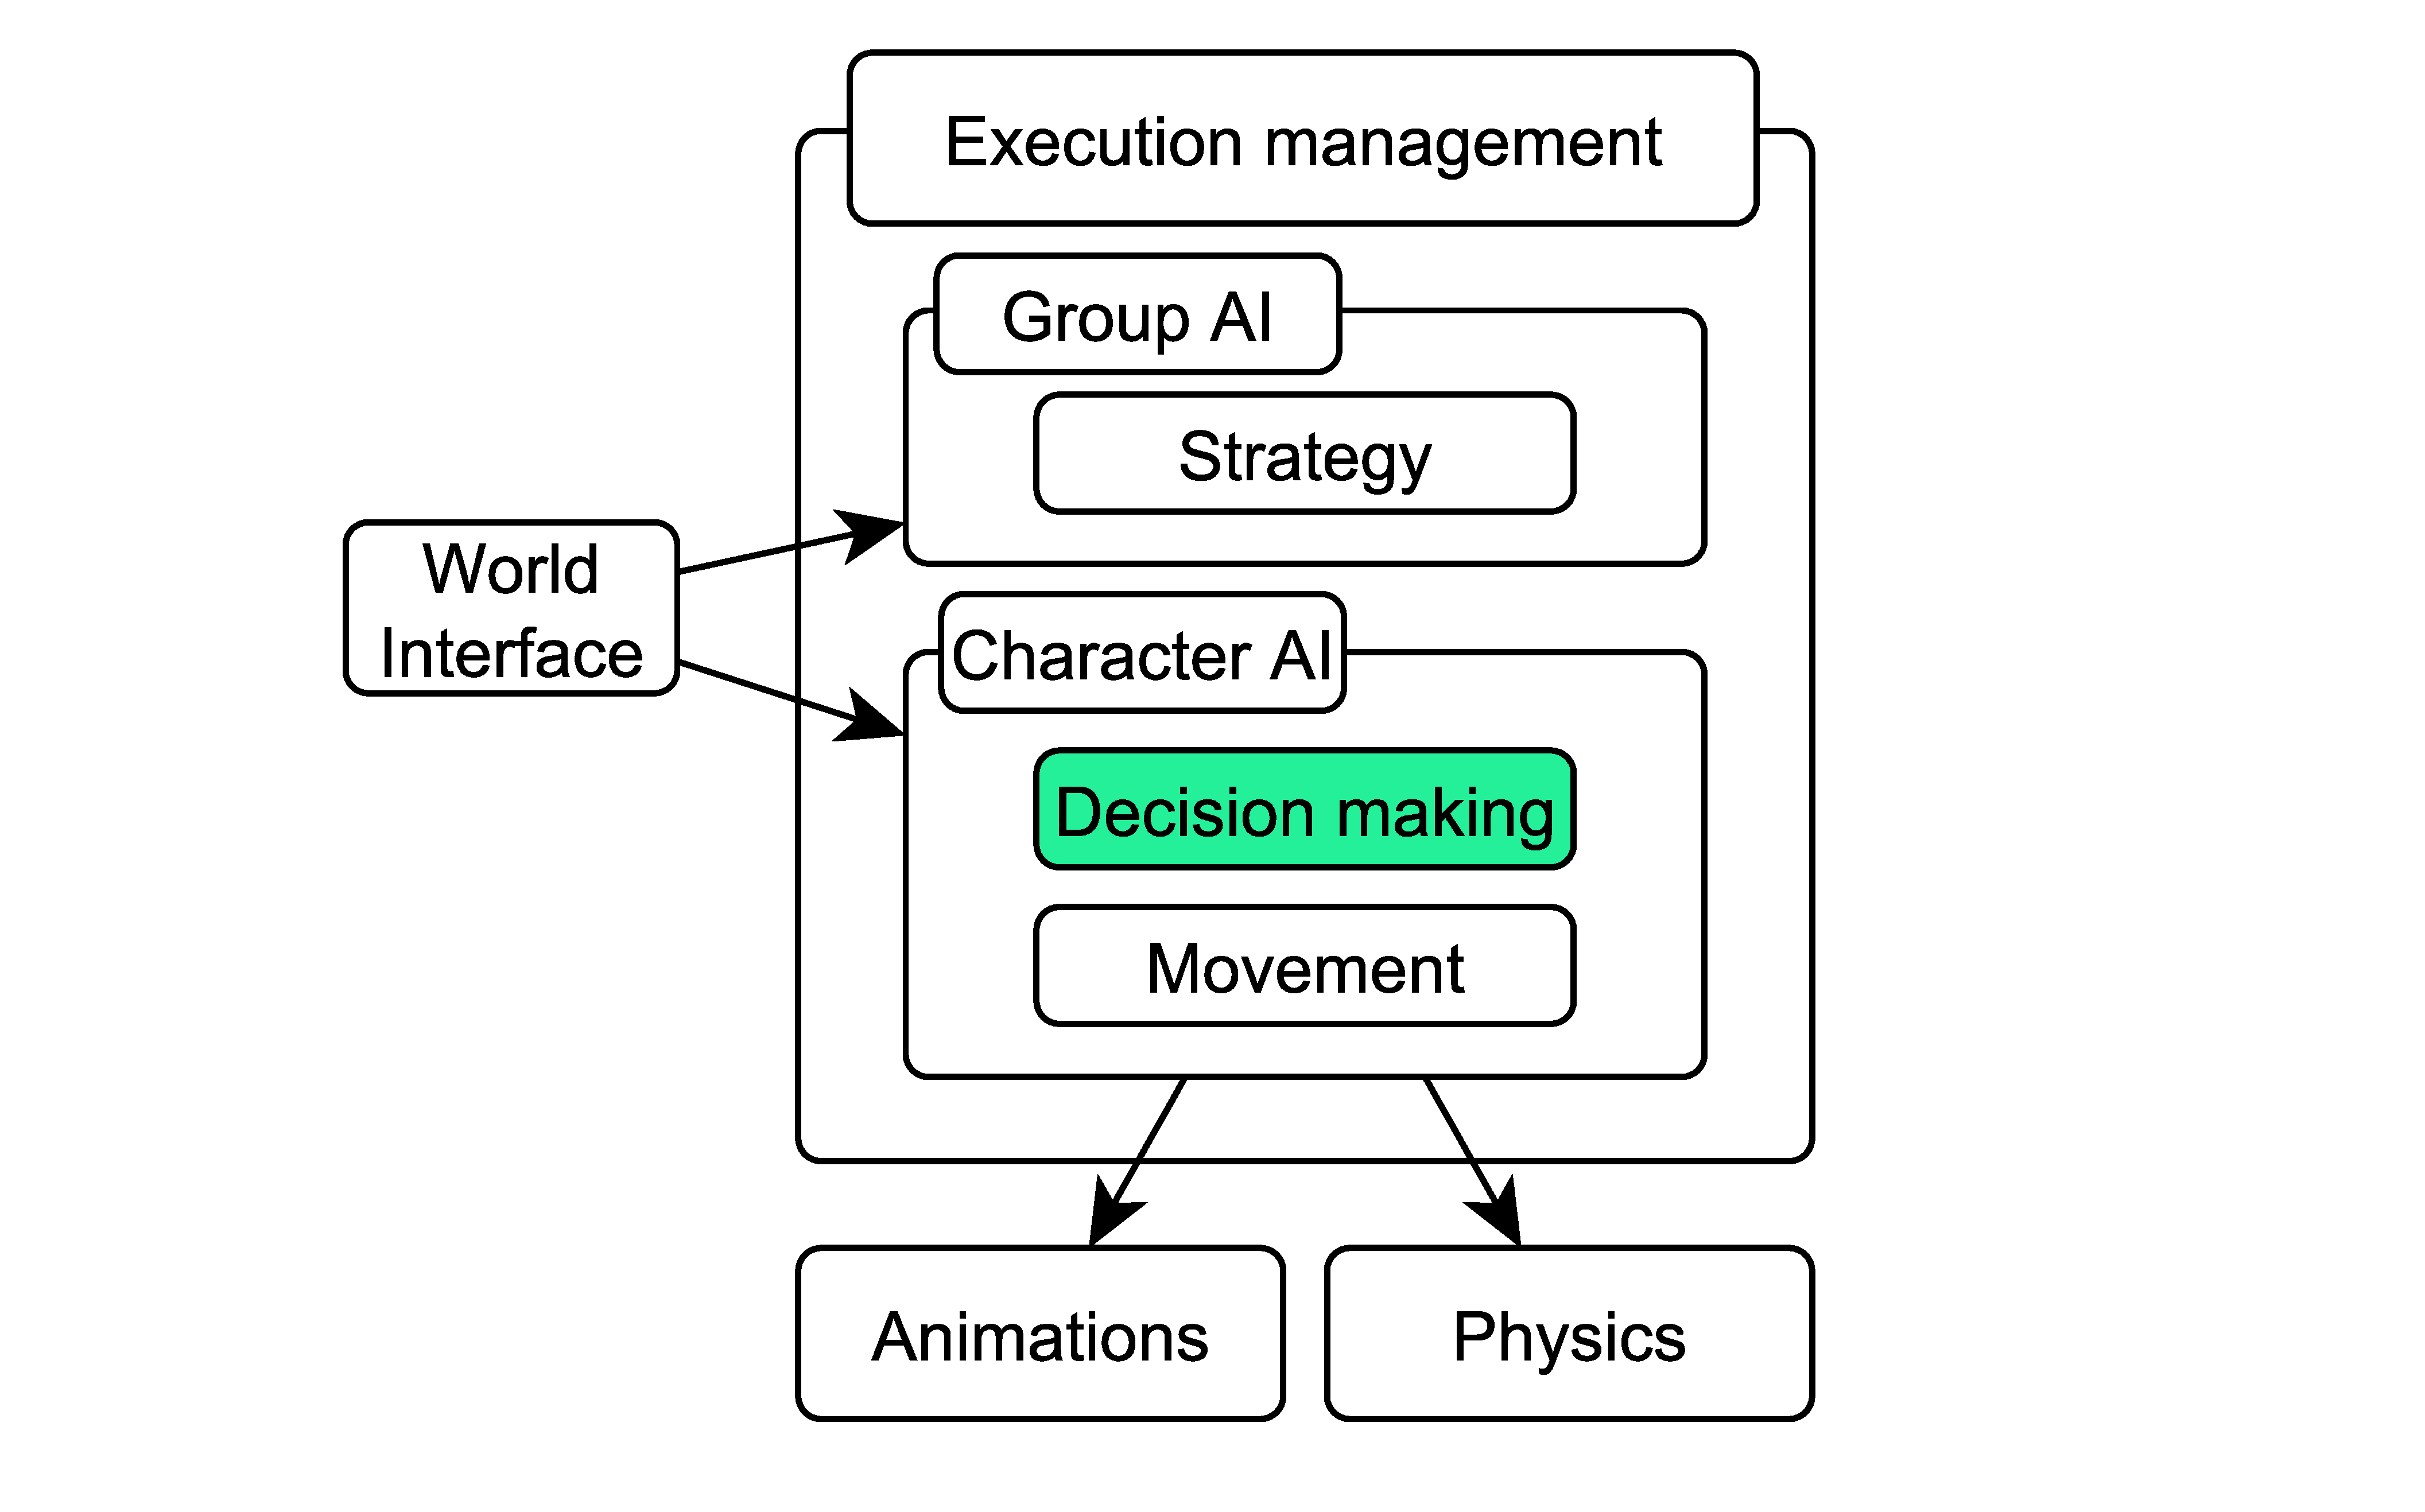
\includegraphics[width=0.9\textwidth]{Videospielentwicklung/game-ai model}
	\captionsetup{justification=justified, format=plain}
  \caption{Game-AI Model: Die Thesis fokussiert sich auf den Bereich der Entscheidungsfindung (\textit{Decisionmaking}) in gr\"{u}n markiert}
  \label{fig:game-ai model}
\end{figure}
\chapter{Entscheidungssysteme}
\label{chap:entscheidungssysteme}

%Man unterscheidet zwischen open-loop und closed-loop Systemen. Bei nondeterministischen environments, also unversehbaren Umgebungen sollten closed-loop Systeme benutzt werden

Die Entscheidungsfindung ist die Entscheidung, welche Aktionen f�r einen NPC gew�hlt werden. Sie wird �ber sogenannte Entscheidungssysteme realisiert. Basierend auf dem Zustand des NPC, f�hren sie verschiedene Aktionen �ber \hyperref[chap:game-objects]{Komponenten} durch. Nach dem Fund der jeweiligen Aktion gibt der Prozessor dem Entscheidungssystem Zeit, die dazugeh�rige Komponente auszuf�hren.

\section{Ad-Hoc Behavioring Authoring}

Zu den popul�rsten Entscheidungssystemen der Game-AI geh�ren die Ad-Hoc Behaviour Authoring Methoden. Zu diesen geh�ren die Finite State Machines (FSM) und Behavior Trees (BT). Die Ad-Hoc Behaviour Authoring Methoden dominieren die Entscheidungsfindung der NPCs in der Game-AI. Bei den Methoden wird die Verhaltensweise der NPCs explizit programmiert. Sie beinhalten normalerweise keine Art von Algorithmen zum Lernen oder Suchen von Entscheidungen. Sie sind leicht zu implementieren, visualisieren und debuggen. Mit der steigenden Komplexit�t der NPCs wird es jedoch schwieriger, das Entscheidungssystem zu designen, erweitern oder anzupassen.

\subsection{Finite State Machine}

Die Finite State Machine (FSM) wird als Graph repr�sentiert. Die FSM speichert dabei Informationen in Knoten, die wiederum Kanten besitzen, die zu weiteren Knoten f�hren. Eine FSM kann sich zu jedem Zeitpunkt nur in einem Knoten befinden. Ein Knotenwechsel erfolgt, wenn die Bedingung f�r die entsprechende Kante erf�llt ist. 

In der Game-AI repr�sentieren die Knoten die Zust�nde des NPC, wie zum Beispiel das Patrouillieren oder Angreifen. Die Zust�nde der Knoten werden �ber \hyperref[chap:game-objects]{Komponenten} ausgef�hrt. So ben�tigt der Zustand des Patrouillierens solche Komponenten, die ihn zu bestimmten Punkten bewegen. Die �berg�nge �ber die Kanten zwischen den Zust�nden erfolgen �ber Bedingungen. So kann ein NPC vom Zustand des Patrouillierens in den des Angreifens wechseln, sobald die Bedingung erf�llt ist, dass der NPC den Spieler sieht. Die NPCs des FPS Half-Life wurde beispielsweise �ber eine FSM realisiert.

\begin{figure}[h]
  \centering
  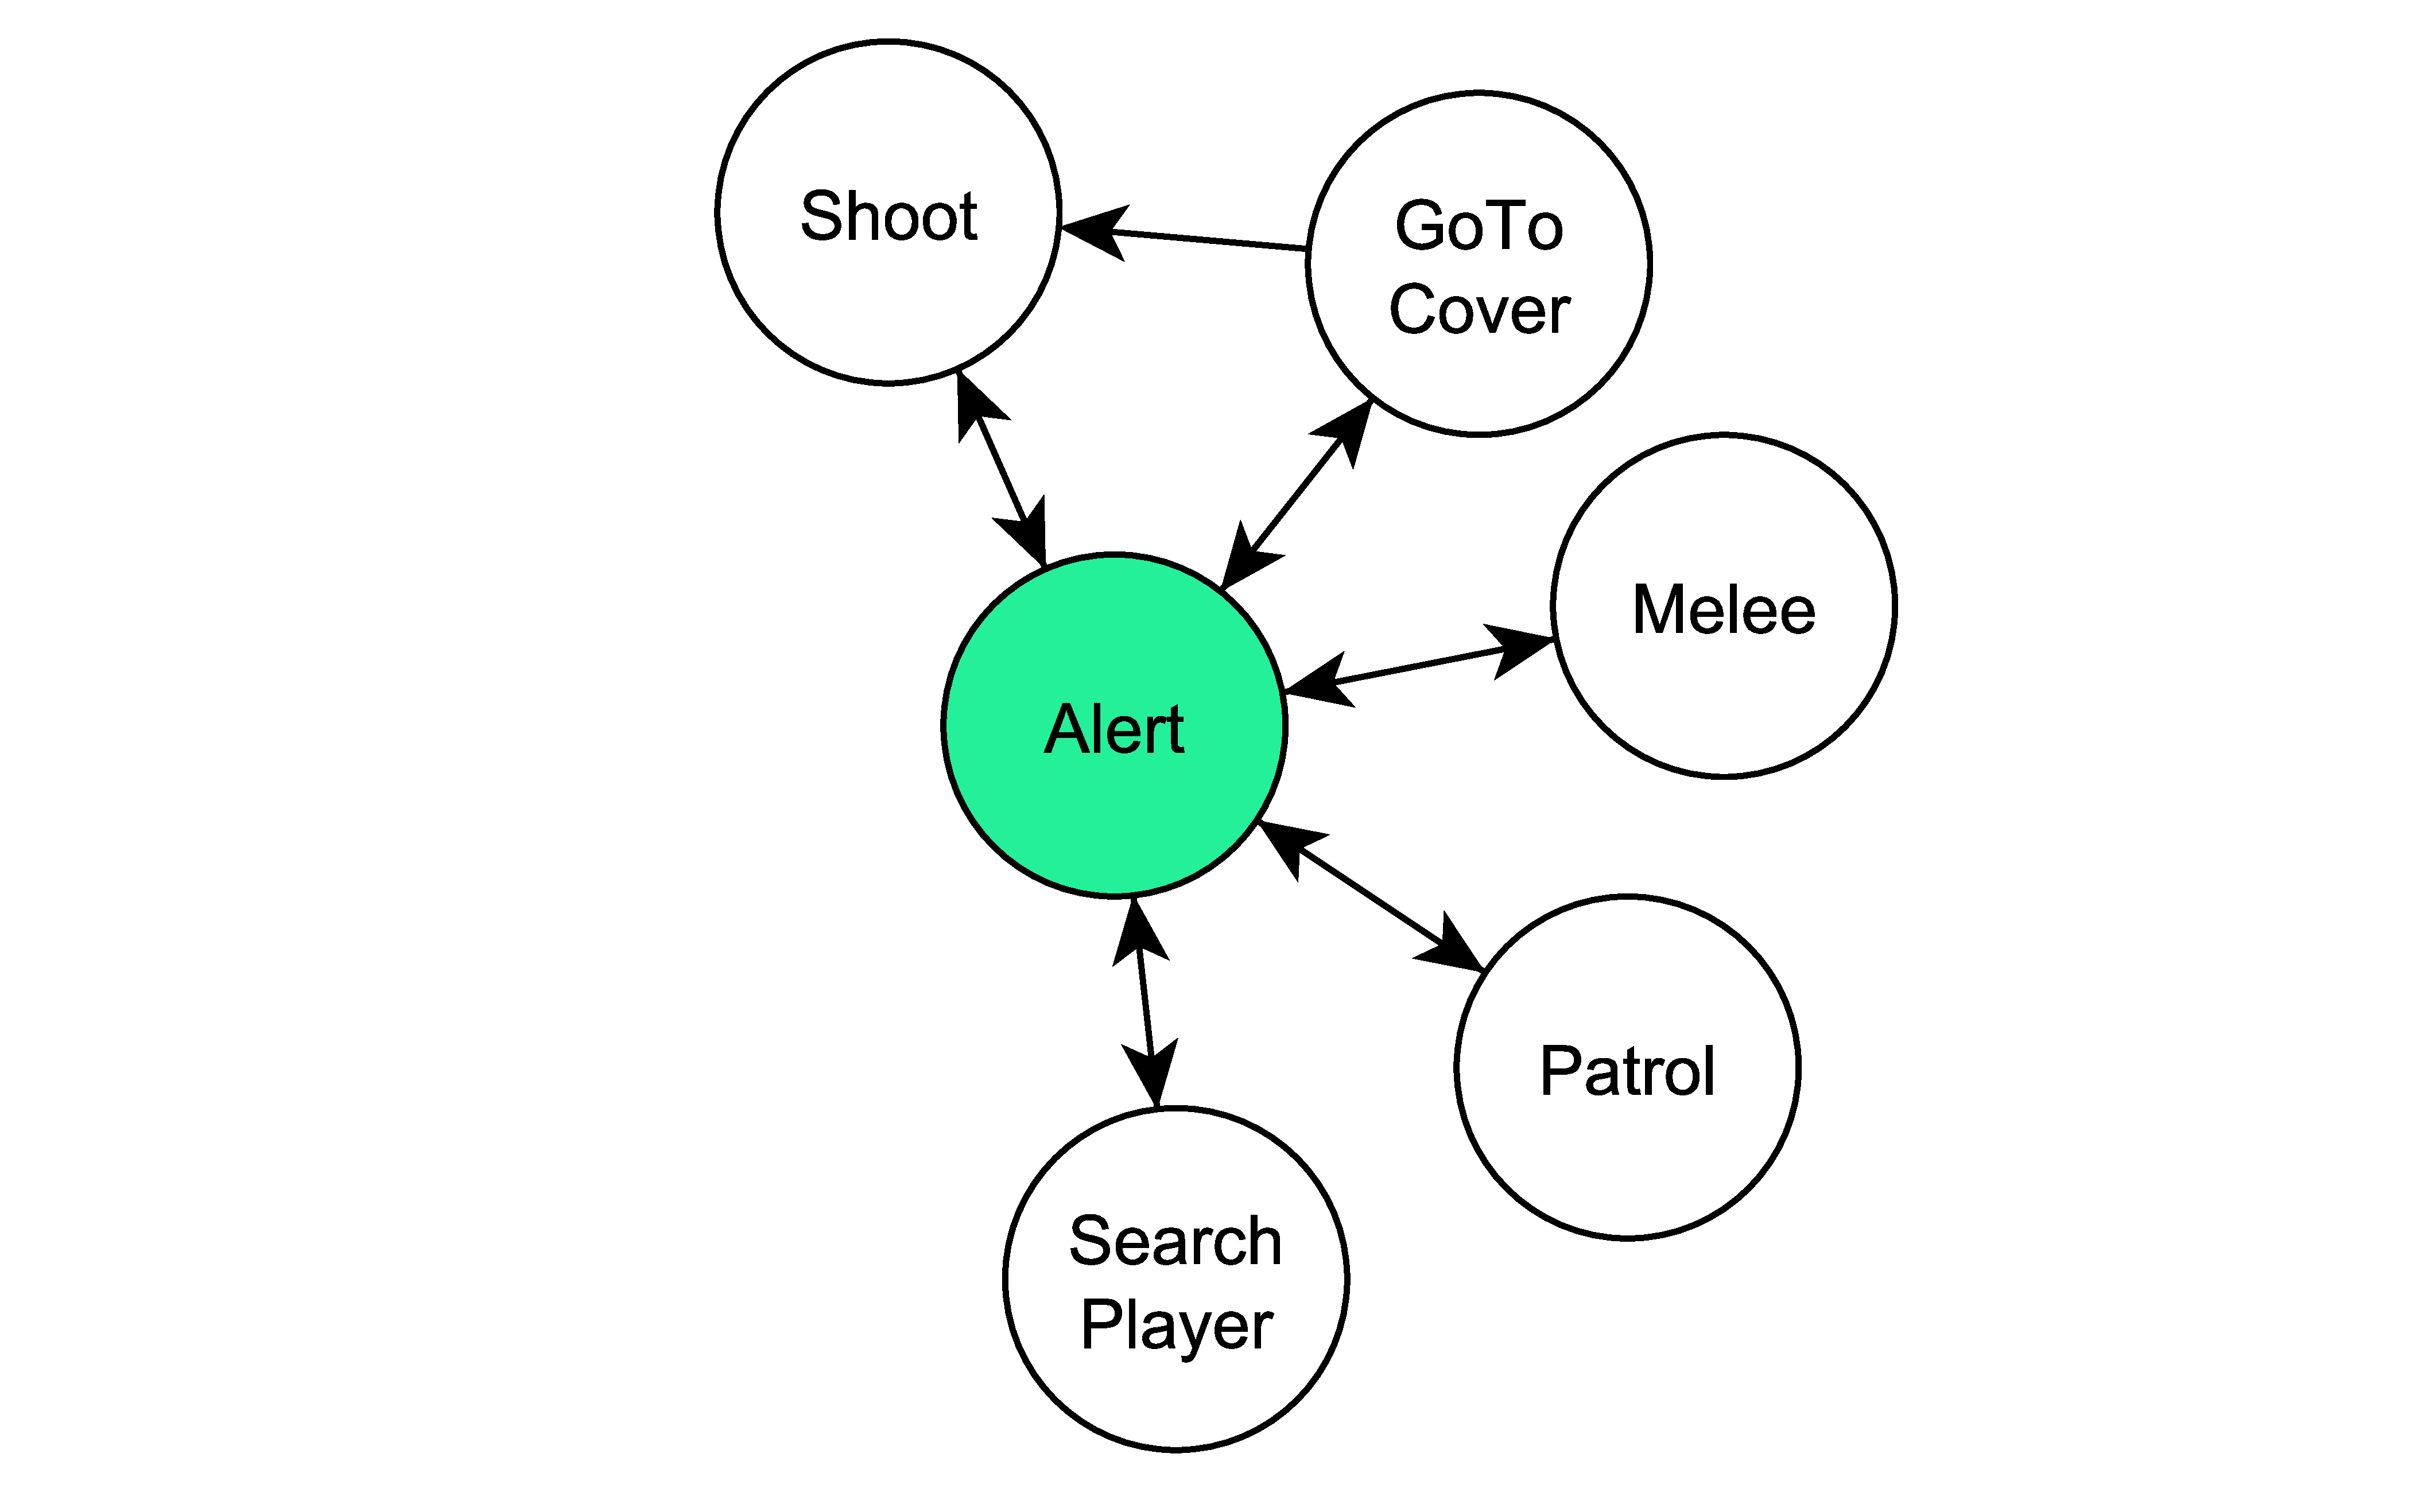
\includegraphics[width=\textwidth]{Entscheidungssysteme/fsm}
	\captionsetup{justification=justified, format=plain}
  \caption{Finite State Machine Beispiel}
  \label{fig:ES FSM}
\end{figure}


\subsection{Behavior Tree}

Der Behavior Tree (BT) wird als Baumstruktur dargestellt. Anders als die FSM besitzt der BT keine Zust�nde, sondern Tasks. Diese Tasks lassen sich in verschiedene Kategorien einteilen und erhalten �ber den Prozessor Zeit, ihr Skript durchzuf�hren.

% Run, Success oder Failure gro� klein?
Nach der Ausf�hrung gibt das Skript des Tasks einen der folgenden Werte zur�ck: Run, Success oder Failure. Run impliziert, dass der Task noch aktiv ist, Success, dass der Task erfolgreich abgeschlossen wurde und Failure, dass der Task fehlgeschlagen ist.

Die Kategorien der Tasks lauten wie folgt: Conditions, Actions und Composites. Die Condition Task pr�ft Bedingungen, die einen Wert wie Success oder Failure zur�ckgibt, wie zum Beispiel, ob der Spieler zu sehen ist. Meistens findet die Ausf�hrung der Condition Task vor der Action Task statt. Die Action Taks f�hrt anschlie�end ihre Aktion �ber \hyperref[chap:game-objects]{Komponenten} des NPC durch, wie zum Beispiel zu schie�en oder in Deckung zu gehen. Beide Task Kategorien sind die Bl�tter der Baumstruktur.

Die dritte Kategorie ist die Composite Task, welche die Sammlung der Child-Tasks, also der Condition- und Action-Tasks, verwaltet. Das Verhalten der Composite Task basiert auf dem resultierenden Wert der Child-Tasks. Die Composite Task l�sst sich in zwei Subkategorien, Sequences und Selectors, aufteilen. Basierend auf dem R�ckgabewert wird entschieden, ob der n�chste Child-Task ausgef�hrt wird oder der Composite stoppt und selbst einen R�ckgabewert zur�ckgibt. So gibt ein Selector den R�ckgabewert Success, sobald einer seiner Child-Tasks Success zur�ckgibt. Sollte ein Child-Task dagegen Failure zur�ckgeben, so wird der n�chste Child-Task ausgef�hrt, bis keine Child-Tasks verf�gbar sind und der Selector folglich Failure an seinen Parent zur�ckgibt. So f�hren Selectors die erstm�gliche Child-Task in ihrem Set aus. Eine Sequence gibt Failure als R�ckgabewert, sobald einer seiner Child-Tasks Failure zur�ckgibt. Erst, wenn alle Child-Tasks Success zur�ckgeben, gibt die Sequence den R�ckgabewert Success zur�ck. Eine Sequence repr�sentiert ein Set an Aktionen, die durchgef�hrt werden m�ssen. Ein Beispiel f�r die Umsetzung des BT als Entscheidungssystem f�r NPCs ist der FPS Halo 2.

\begin{figure}[h]
  \centering
  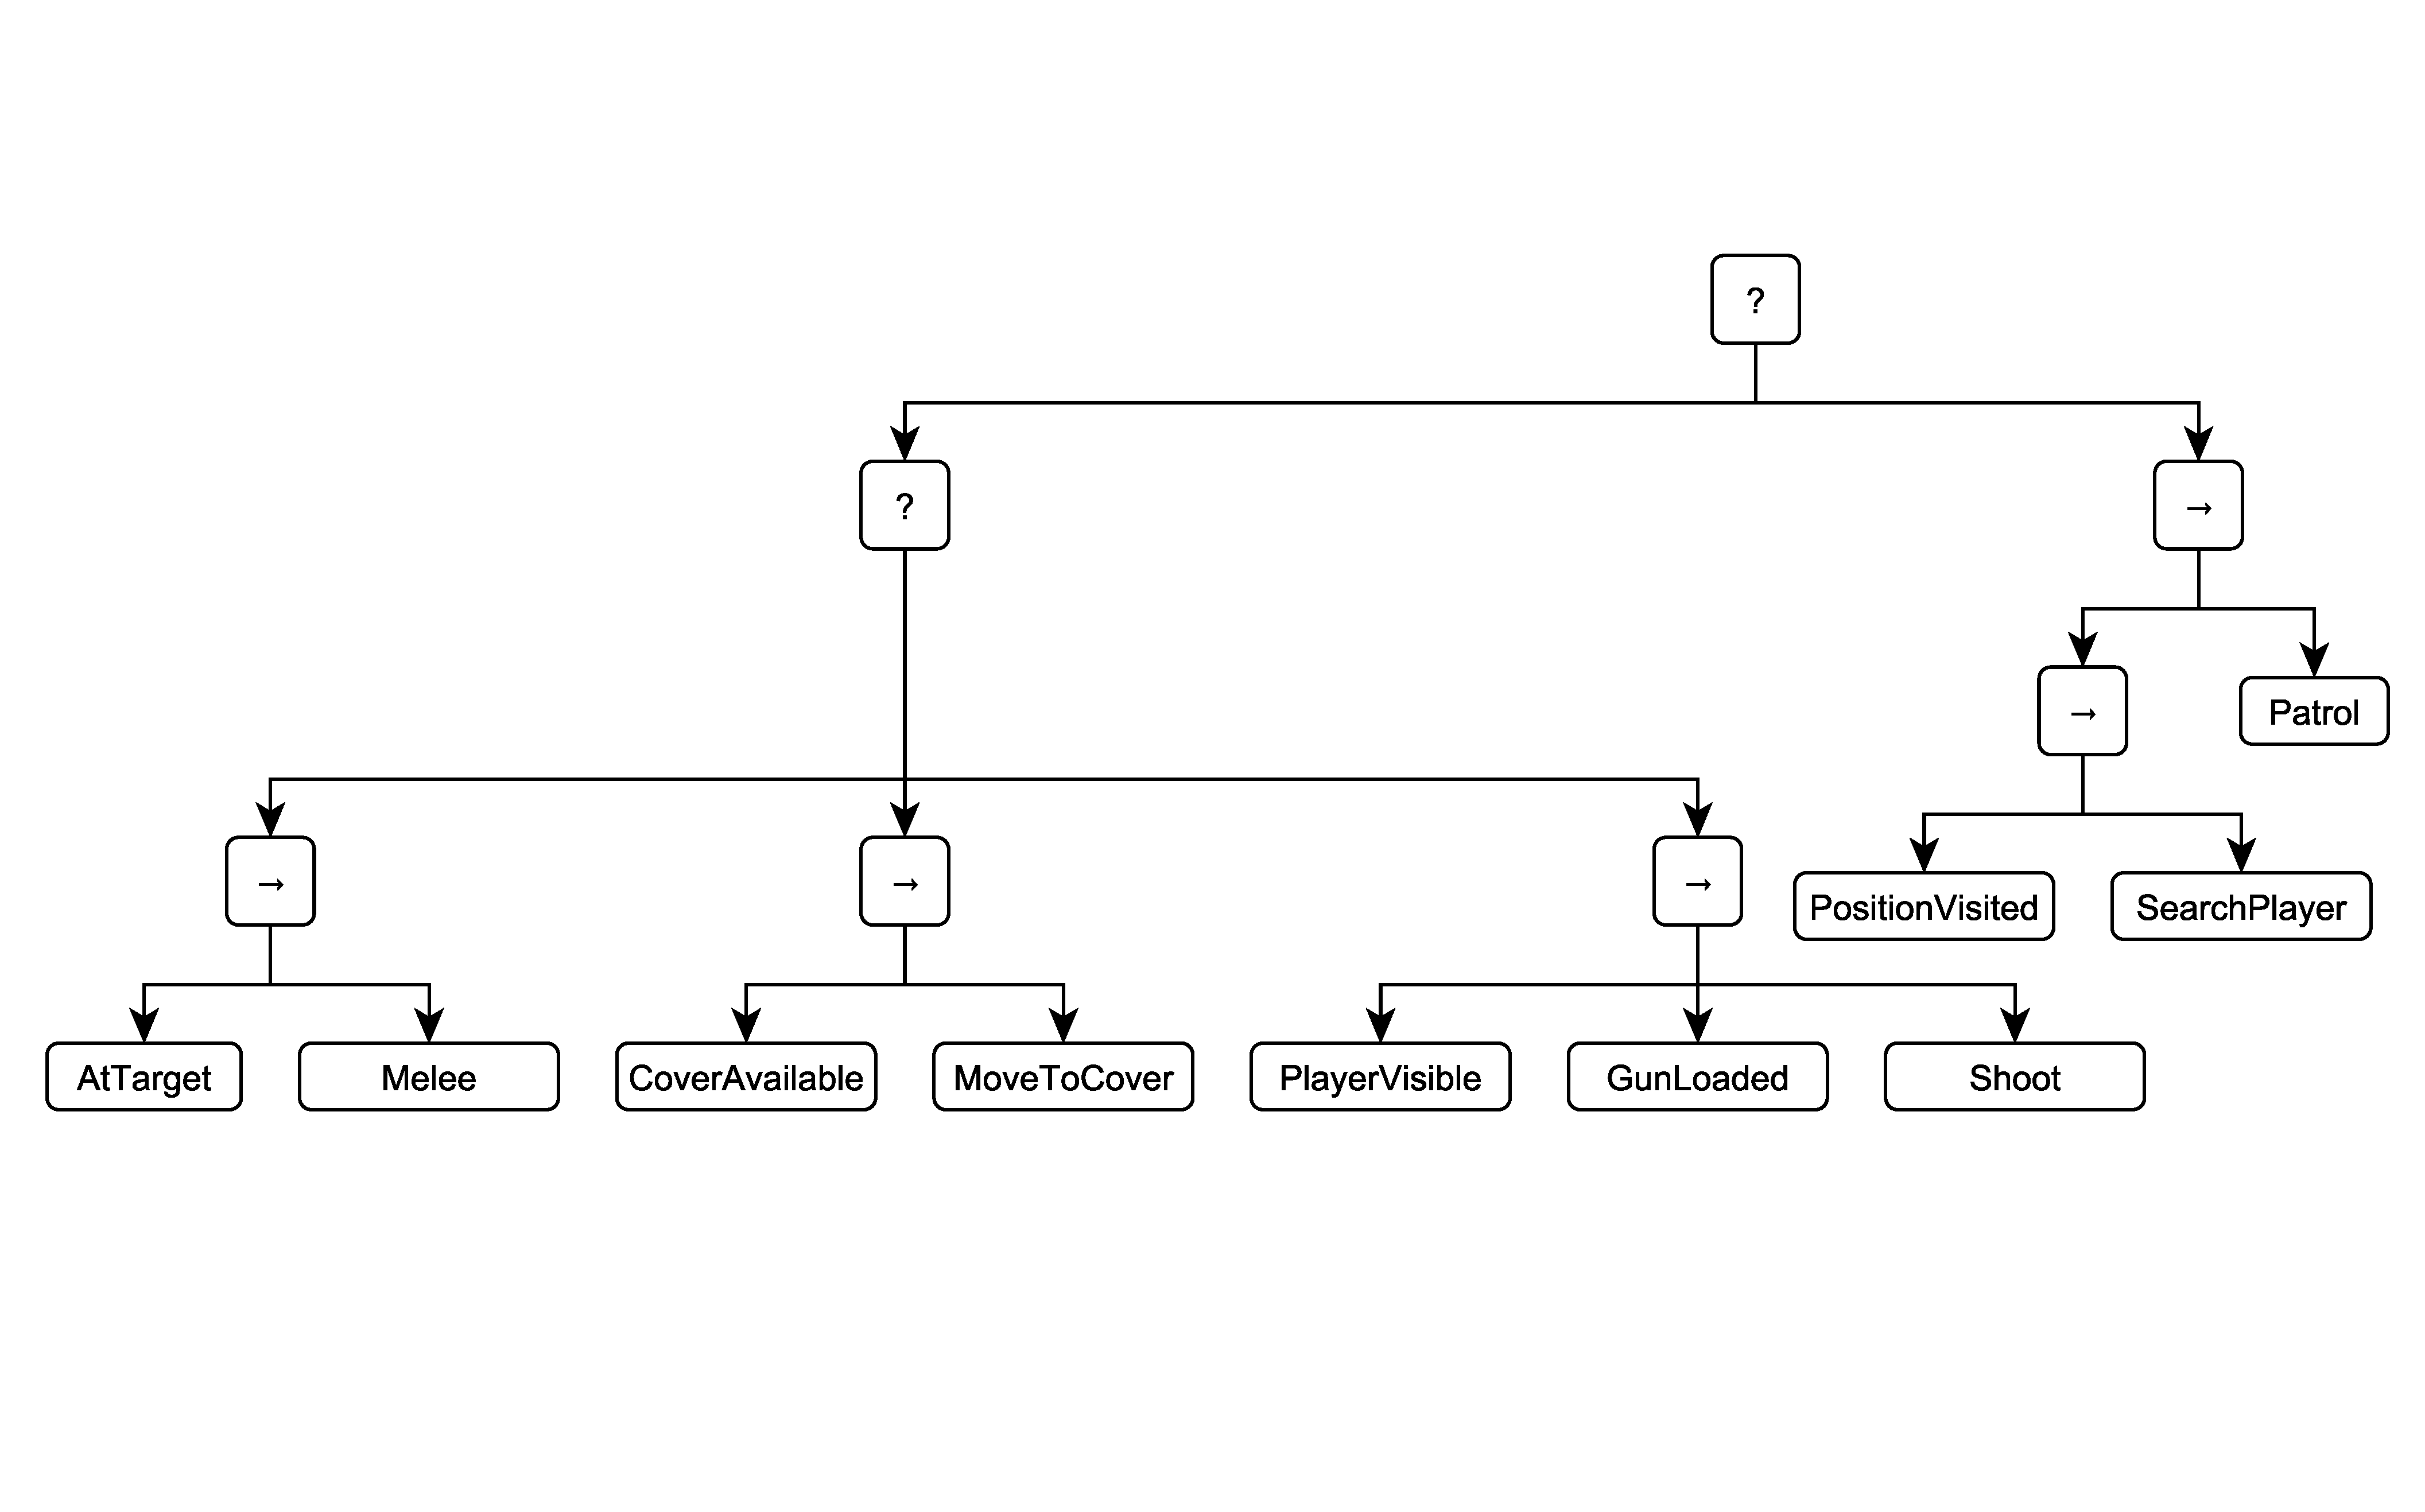
\includegraphics[width=\textwidth, trim=0cm 10cm 0cm 5cm, clip]{Entscheidungssysteme/behavior tree}
	\captionsetup{justification=justified, format=plain}
  \caption{Behavior Tree Beispiel an einem FPS-NPC}
  \label{BT}
\end{figure}

%Andrere Quellen
 Oneachupdate, aBTperformsadepth-first traversaluntil a lowlevelbehaviour (representedbya leafnode)has either succeeded or is set to the" running" state. \autocite{qlbt}

\section{Suchalgorithmen}

% �ndern
Aufgaben der AI k�nnen auch als Suchprobleme formuliert werden, die durch das Finden des besten Pfades gel�st werden. Die Suchalgorithmen konstruieren einen Suchbaum, bei dem der Wurzelknoten den Ausgangszustand darstellt, die Kanten die Operationen des Agenten repr�sentieren, die zu einem neuen Knoten f�hren, welcher einen neuen Zustand repr�sentiert. Aus einem Zustand sind mehrere Operationen m�glich. Einer der bekannteren Suchalgorithmen ist der Monte Carlo Tree Search (MCTS), welcher Bestandteil von AlphaGo ist. Ein weiterer bekannter Suchalgorithmus ist A*, welcher sowohl die Navigation der NPC als auch die Entscheidungsfindung in GOAP realisiert.

\section{Entscheidungssysteme in der Robotik}

\subsection{Finite State Machine}

Bei der Entwicklung eines Roboter-Verhaltens wird darauf geachtet, dass die vielen \hyperref[chap:game-objects]{Komponenten}, die f�r das Verhalten n�tig sind, m�glichst effizient zusammenarbeiten. Eine der simpelsten Architekturen f�r die Umsetzung eines Roboter Verhaltens ist die Finite State Machine (FSM).

Ein Beispiel ist ein Linien-Folgender-Roboter, der mithilfe von FSM umsetzbar ist. Die FSM bestimmt die Aktion auf Basis des aktuellen Knotens des Roboters. Der Roboter kann seinen Knoten und damit seine Aktion wechseln. Wenn ein Sensor des Roboters beispielsweise erkennt, dass er sich nicht mehr innerhalb der schwarzen Linie bewegt, dann wechselt er in einen anderen Knoten, der durch seine Aktionen den Kurs des Roboters korrigiert.

\subsection{Behavior Tree}

Der Behavior Tree (BT) ist ein weiteres Entscheidungssystem in der Robotik und stammt urspr�nglich aus der Spielentwicklung \ref{}. Wie auch die FSM, wird der BT f�r die Aufgabenorchestrierung eines Roboters eingesetzt. Im Vergleich zu der FSM ist der BT zwar komplexer umzusetzen, hat aber folgende Vorteile: Aktionen k�nnen im BT leichter wiederverwendet und erweitert werden. Zudem muss der BT nicht definieren, wie eine Aktion im Bezug zu einer nachfolgenden Aktion steht.

Ein Konzept f�r die Nutzung eines BT in der Robotik ist die Umsetzung auf einem unbemannten Luftfahrzeug (UAV). Dabei kann der BT als Controller f�r einen Luftkampf dienen.

\subsection{Stanford Research Institute Problem Solver (STRIPS)}

Zu dem Entscheidungssystem Goal Oriented Action Planner (GOAP) gibt es wenige Studien in dem Bereich der Robotik. Daraus l�sst sich schlie�en, dass der GOAP eine untergeordnete Rolle in der Robotik spielt. Der GOAP basiert auf dem �lteren Entscheidungssystem Stanford Research Institute Problem Solver (STRIPS), der wiederum im Roboter Shakey eingesetzt wurde.

Der STRIPS wurde erstmals f�r den mobilen Roboter mit dem Nicknamen Shakey als Plansystem f�r die Aktionen implementiert. Dieser Roboter wurde von 1966 bis 1972 als wissenschaftliches Projekt im Labor f�r k�nstliche Intelligenz des Stanford Research Institutes entwickelt. Das Ziel dieses Projekts war es, Konzepte und Techniken der k�nstlichen Intelligenz zu entwickeln. Diese Konzepte sollen Automaten erm�glichen, in realistischen Umgebungen unabh�ngig zu agieren. Insbesondere boten sie den Kontext und die Motivation f�r die Entwicklung des A*-Suchalgorithmus\autocite{}. Der Roboter konnte nach seiner Fertigstellung in R�umen fahren, Hindernisse und �nderungen in der Umgebung erkennen sowie Boxen verschieben. Gab man dem Roboter ein Ziel als logische-Formel, so sollte der STRIPS eine g�ltige Sequenz an solchen Aktionen zur�ckgeben, die nach ihrer Ausf�hrung das Ziel erreichen sollen.

Der STRIPS besteht aus den folgenden Modulen: Einen Ausgangszustand, gegebenen Zielzustand und eine Sammlung an Aktionen.

Der Ausgangszustand repr�sentiert das derzeitige Wissen �ber die Welt des Agenten, also seinen Status. Im Falle von Shakey k�nne es sich um die Position handeln, in der sich der Roboter befindet und das Wissen �ber seine Umwelt, wie zum Beispiel die Verbindung der R�ume.

Die Aktionen haben Effekte und Vorbedingungen. Die Vorbedingungen einer Aktion entscheiden, ob es m�glich ist, diese in die Sequenz aufzunehmen. Die Effekte werden �ber eine Add- und Delete-List realisiert. W�hrend die Delete-List Wissen �ber Zust�nde l�scht, f�gt die Add-List neues Wissen �ber Zust�nde hinzu. Durch die Durchf�hrung der Add- und Delete-List werden Zust�nde, wie der Ausgangszustand, ge�ndert.

Der Zielzustand wurde im Falle von Shakey durch die logische-Formel von dem Benutzer gegeben. STRIPS baut aus dem Ausgangszustand eine Sequenz an Aktionen, die daraufhin in ihrer Reihenfolge ausgef�hrt werden. Die Ausf�hrung der Aktionen und ihrer Effekte soll den Ausgangszustand so ver�ndern, dass der Agent zu seinem Zielzustand kommt.

Um eine Sequenz an Aktionen zu erzeugen, muss STRIPS die Effekte und Vorbedingungen seiner Aktionen kennen. Hierf�r pr�ft STRIPS, ob der Zielzustand bereits durch den Ausgangszustand erf�llt ist. Sollte der Zielzustand nicht erf�llt sein, w�hlt STRIPS eine Aktion aus, deren Effekte den Zielzustand am ehesten erreichen k�nnen. Dabei wird nach einer Aktion gesucht, deren Add- und Delete-Listen dazu beitragen k�nnen, den Zielzustand zu erreichen. Sollte die relevante Aktion nicht erf�llte Vorbedingungen durch das derzeitige Zustandsmodell besitzen, werden die Vorbedingungen als Unterziel hinzugef�gt und m�ssen ebenfalls durch andere Aktionen erf�llt werden. Wenn mehrere relevante Aktionen gefunden werden, dann f�hrt dies zu einem Suchbaum. Der Prozess wird so lange wiederholt, bis alle Unterziele erf�llt sind. Sobald die Unterziele erf�llt sind, wird das Ausgangsmodell basierend auf der Add- und Delete-List der Aktionen in ein neues Zustandsmodell transformiert. Dieses neue Zustandsmodell repr�sentiert eine hypothetische Welt, die durch die Anwendung der ausgew�hlten Aktion entsteht. Es wird als neuer Ausgangspunkt f�r die n�chste Selektion einer Aktion verwendet, um den Zielzustand schrittweise zu erreichen. Sollte der neue Ausgangspunkt nicht dem Zielzustand entsprechen, wird der Prozess fortgesetzt. Entspricht der Ausgangspunkt schlie�lich dem Zielzustand, so wurde ein Plan an Aktionen gefunden. 

\chapter{Suchproblem und Suchalgorithmen}
\label{chap:suchproblem und suchalgorithmen}

Ein Agent muss f\"{u}r ein bestimmtes Ziel die richtige Auswahl an Aktionen treffen, die nach ihrer Ausf\"{u}hrung den Zielzustand erreichen. Der Prozess der Bestimmung der Abfolge von Aktionen wird als Suche bezeichnet und mithilfe von Suchalgorithmen, wie A*, durchgef\"{u}hrt. F\"{u}r diesen Prozess ben\"{o}tigt der Agent einen solchen Raum mit Regeln und Informationen, der im Suchproblem definiert wird. Ein Suchalgorithmus sucht die richtige Auswahl an Aktionen und gibt sie in eine Aktions-Sequenz wieder. Die Suche der Aktionen geschieht \"{u}ber einen Suchbaum, der durch das Suchproblem definiert wird. Die Informationen des Kapitels basieren auf den wissenschaftlichen Arbeiten \autocite{RN2020, 4082128, Felner2011}.

\section{Suchproblem}
\label{chap:suchproblem}

Ein Suchproblem wird durch einen Satz m\"{o}glicher Zust\"{a}nde, einen Ausgangszustand, Zielzust\"{a}nde, Aktionen, ein \"{U}bergangsmodell und Aktionskosten definiert. Ein Satz m\"{o}glicher Zust\"{a}nde beschreibt die Umwelt des Agenten. Der Ausgangszustand $s$ gibt den Zustand an, von dem der Agent startet. Zielzust\"{a}nde definieren ein oder mehrere Ziele, die der Agent verfolgt.


\begin{align}
	s = \{\textit{AtCover}, \textit{GunLoaded}, \textit{PlayerAlive}\}
\end{align}


Die Aktionen des Agenten k\"{o}nnen in bestimmten Zust\"{a}nden \textit{ACTIONS}$(s)$ ausgef\"{u}hrt werden.

\begin{align}
	\textit{ACTIONS}(\textit{GunLoaded}) &= \{\textit{Shoot}\} \\
	\textit{ACTIONS}(\lnot \textit{GunLoaded}) &= \{\textit{Reload}\}
\end{align}

Ein \"{U}bergangsmodell \textit{TRANSITION}$(s,a) = s^*$ beschreibt den resultierenden Zustand $s^*$, der aus einer Aktion $a$ im derzeitigen Zustand $s$ resultiert.

\begin{align}
	\textit{TRANSITIONS}(\textit{GunLoaded}, \textit{Shoot}) &= \lnot \textit{PlayerAlive}
\end{align}

Durch eine Aktion-Kosten-Funktion \textit{ACTIONCOST}$(s,a,s^*)$ erh\"{a}lt man die Kosten einer Aktion $a$, die in einem Zustand $s$ ausgef\"{u}hrt wird und in einen neuen Zustand $s^*$ f\"{u}hren.

\section{Suchbaum}
\label{chap:suchbaum}

Die L\"{o}sung eines Suchproblems ist eine Aktionssequenz, die nach ihrer Ausf\"{u}hrung den Ausgangszustand in den Zielzustand \"{u}berf\"{u}hrt. Die Suche nach einer solchen Aktions-Sequenz geschieht \"{u}ber einen Suchbaum.

Ein Suchbaum ist eine Baumstruktur, die in der Informatik f\"{u}r das speichern von Daten benutzt wird. Die Struktur basiert auf einer Anordnung von Knoten, die mit anderen Knoten durch Kanten verbunden sind. Diese Knoten speichern, je nach Anwendung bestimmte Daten. Wenn der Suchbau einen Wurzelknoten, von dem aus s\"{a}mtliche anderen Knoten erreichbar sind oder der seinerseits von jedem anderen Knoten aus erreicht werden kann, handelt es sich um einem Wurzelbaum. Es gibt verschiedene Typen von Suchb\"{a}umen, die sich in ihren Eigenschaften und Zwecken unterscheiden, wie zum Beispiel Bin\"{a}re Suchb\"{a}ume oder AVL-B\"{a}ume. In Abbildung \ref{fig:suchabaum aufbau} wird ein abstrakter Suchbaum dargestellt.

\begin{figure}[h]
  \centering
  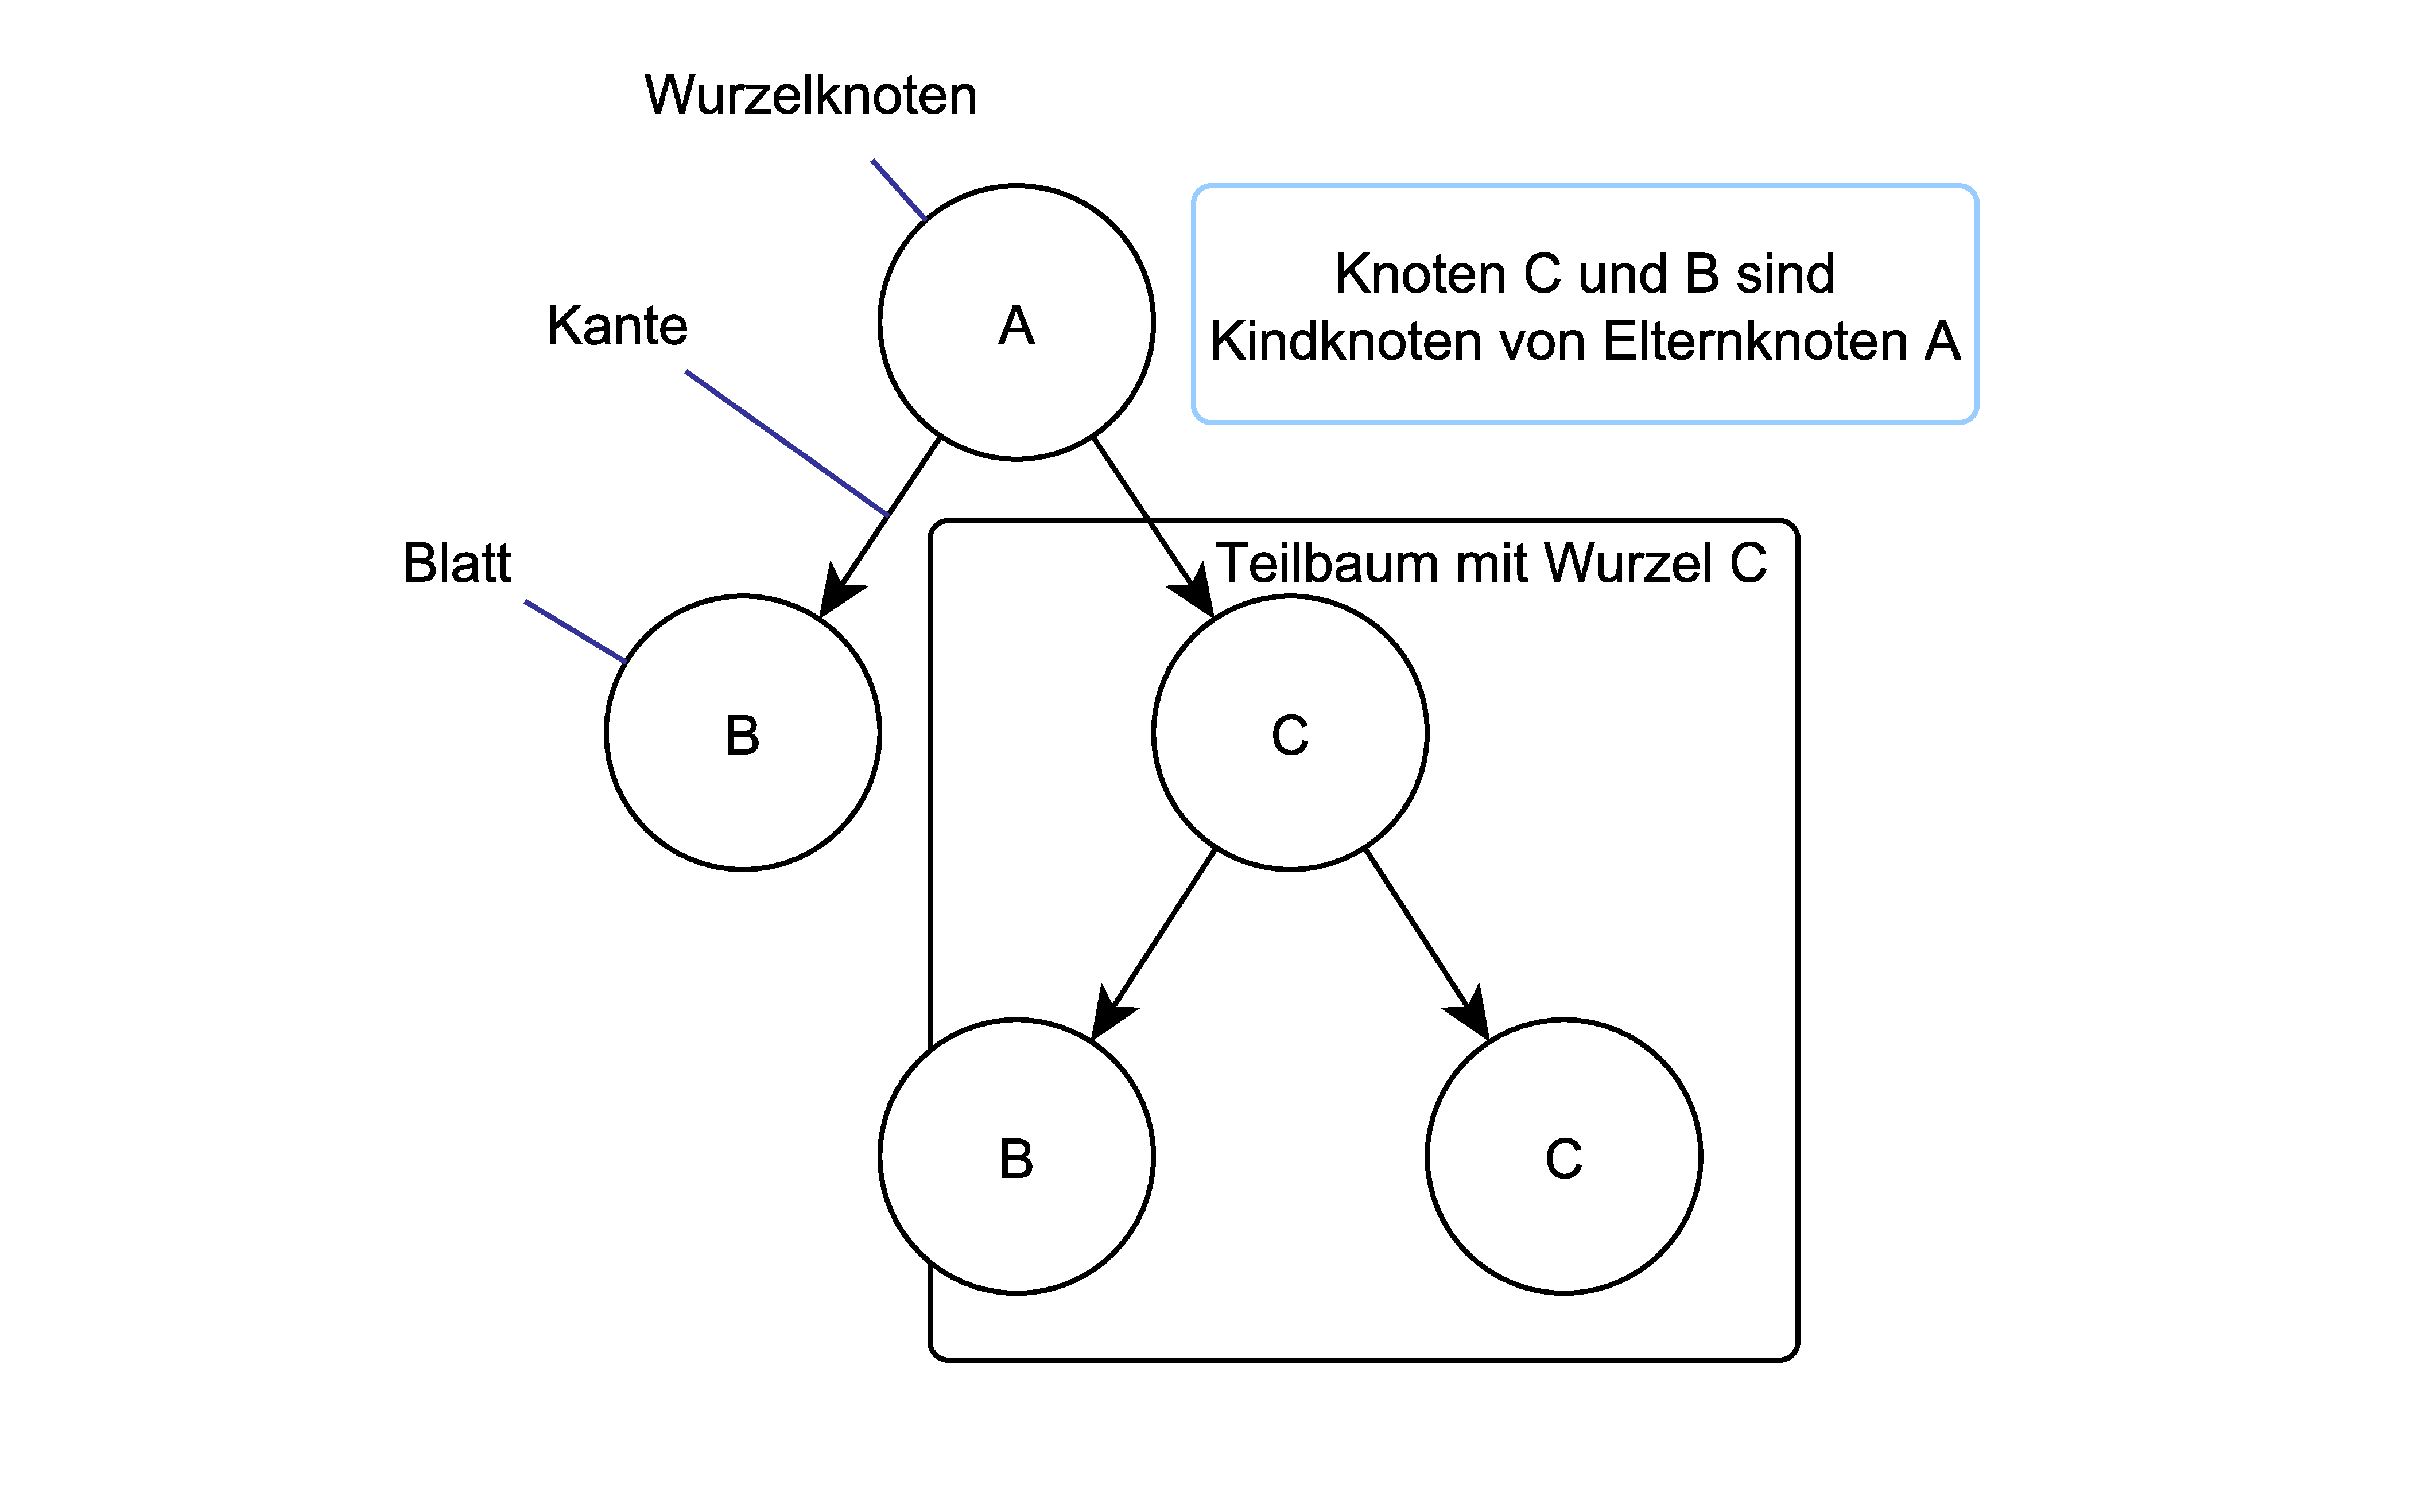
\includegraphics[width=0.7\textwidth]{Suchalgorithmen/suchbaum aufbau.pdf}
	\captionsetup{justification=justified, format=plain}
  \caption{Suchbaum Aufbau}
  \label{fig:suchabaum aufbau}
\end{figure}

\subsection{Knoten eines Suchbaums}
\label{chap:knoten eines suchbaums}

Ein Knoten speichert dabei:
\begin{itemize}
	\item Einen Zustand, zu dem die Aktion des jeweiligen Knoten gef\"{u}hrt hat
	\item Eine Aktion, die auf dem Eltern-Knoten ausgef\"{u}hrt wurde
	\item Einen Eltern-Knoten, auf dem die Aktion durchgef\"{u}hrt wurde und den jeweiligen Knoten generiert hat
	\item Die Pfad-Kosten, der die summierten Kosten vom Ausgangsknoten bis zu dem jeweiligen Knoten speichert
\end{itemize}

\subsection{Gerichtete und ungerichtete Suchb\"{a}ume} \label{gerichtete Graphen}
\label{chap:gerichtet und ungerichtete suchb\"{a}ume}

Die Kanten eines Suchbaums bestimmten ob dieser gerichtet oder ungerichtet ist. In einem ungerichteten Suchbaum sind die Kanten zwischen den Knoten bidirektional, sodass sie keine feste Richtung vorgeben. Wenn eine Kante in einem ungerichteten Suchbaum die Knoten A und B verbindet, dann ist die Kante in beide Richtungen durchquerbar. Wodurch man mit der Kante sowohl von A nach B, als auch von B nach A navigieren kann. In einem ungerichteten Suchbaum kann jeder Knoten der Wurzelknoten sein. Bei einem gerichteten Suchbaum verbindet eine Kante zwei Knoten, wobei eine klare Richtung von einem Knoten zu dem anderen Knoten vorgegeben ist. Das bedeutet, dass die Kante nur in eine Richtung durchquerbar ist: vom Elternknoten zu dem Kindknoten.

\subsection{Balancierte und unbalancierte Suchb\"{a}ume}
\label{chap:balancierte und unbalancierte suchb\"{a}ume}

Eine Eigenschaft des Suchbaums ist die Balance, die ihn als balanciert oder unbalanciert klassifiziert. Die Klassifizierung basiert auf der Anordnung der Knoten, insbesondere auf deren H\"{o}he. Die H\"{o}he entspricht der maximalen Anzahl an Kanten von der Wurzel bis zu einem Blatt. Bei einem balancierten Suchbaum, deren H\"{o}he so optimiert ist, dass Such-, Einf\"{u}ge- und L\"{o}schoperationen effizient durchgef\"{u}hrt werden k\"{o}nnen. Dabei sind die Knoten m\"{o}glichst gleichm\"{a}\ss{}ig verteilt, um eine \"{u}berm\"{a}\ss{}ige Baumh\"{o}he zu vermeiden. Der H\"{o}henunterschied zwischen den linken und rechten Teilb\"{a}umen darf h\"{o}chstens 1 betragen. Ein Baum gilt als unbalanciert, wenn der H\"{o}henunterschied gr\"{o}\ss{}er als 1 ist.

\section{Suchalgorithmen}
\label{chap:suchalgorithmen}

Das Suchproblem soll mit seinen Informationen durch einen Suchalgorithmus gel\"{o}st werden. Ein Suchalgorithmus sucht \"{u}ber einen Suchbaum einen Pfad zu dem Ziel. Wie effizient der gefundene Weg, h\"{a}ngt von dem Suchalgorithmus ab. 

Im Bereich der Suchalgorithmen wird zwischen informierten und uniformierten Algorithmen unterschieden. Informierte Algorithmen k\"{o}nnen die Distanz zu dem Ziel mithilfe einer Heuristik sch\"{a}tzen, w\"{a}hrend uniformierte eine solche Sch\"{a}tzung nicht durchf\"{u}hren k\"{o}nnen. Ein weiterer Unterschied ist die Zeit und Speicherkomplexit\"{a}t. W\"{a}hrend uninformierte Algorithmen wie die Tiefensuche weniger Speicher ben\"{o}tigen, k\"{o}nnen sie ineffizient sein, da sie keine Richtung zu dem Ziel ber\"{u}cksichtigen. Informierte Algorithmen sind speicherintensiver, k\"{o}nnen aber Pfade schneller durch die Informationen der Heuristik finden. Unter die uninformierten Suchalgorithmen fallen die Breitensuche, Dijkstra und Tiefensuche. Zu den informierten Suchalgorithmen geh\"{o}rt unter anderem die Bestensuchen.


\subsection{Expansion einer Bestensuche}
\label{chap:bestensuche}

Zu den informierten Suchalgorithmen geh\"{o}rt unter anderem die Bestensuche. Der Algorithmus wird im Pseudocode \ref{lst:pseudo bestensuche} erläutert. Eine Bestensuche arbeitet sich schrittweise \"{u}ber Iterationen mithilfe von Expansionen zu einem Zielknoten vor. Vor der ersten Iteration wird ein Wurzelknoten mit dem Ausgangszustand generiert und der offenen Liste hinzugef\"{u}gt. Die offenen Liste stellt dabei eine Priorit\"{ä}ts-Warteschlange dar. So wird sichergestellt, dass bei der ersten Iteration der Wurzelknoten betrachtet wird.

In der Iteration werden Knoten aus der offenen Liste expandiert. Bei einer Expansion ermittelt der Algorithmus mithilfe der Funktion \textit{TRANSITIONS}$(n)$ alle m\"{o}glichen Kanten \textit{ACTIONS}$(n)$, die vom aktuellen Knoten $n$ ausgehen und zu Kindknoten f\"{u}hren. F\"{u}r die Kindknoten wird eine Bewertung durch die Bewertungsfunktion $f(n)$ berechnet, die je nach Suchalgorithmus variiert. Diese Kindknoten werden daraufhin sortiert nach ihrer Bewertung der offenen Liste hinzugef\"{u}gt. Wenn ein Knoten expandiert wird, wird dieser aus der offenen Liste entfernt. Sollte der gelesene Knoten dem Ziel entsprechen, terminiert der Algorithmus und gibt den Knoten zur\"{u}ck. Ansonsten wird dieser expandiert und die resultierenden Kindknoten der offenen Liste hinzugef\"{u}gt. Die Iteration wird solange fortgef\"{u}hrt bis der Zielknoten gefunden wurde oder sich keine Knoten in der offenen Liste befinden und somit keine Knoten zu dem Ziel f\"{u}hren.

Zu den Bestensuchen geh\"{o}rt unter anderem der Greedy best-first-search und der A*"=Algorithmus, die sich in ihrer Bewertungsfunktion unterscheiden.

Die Abbildung \ref{fig:bestensuche beispiel} veranschaulicht eine abstrakte Suche in einem Suchbaum unter Verwendung der Bestensuche. Dabei sind die gr\"{u}nen Knoten bereits expandierte Knoten, w\"{a}hrend die blauen Knoten zur offenen Liste geh\"{o}ren. Gestrichelte Knoten und Kanten repr\"{a}sentieren nicht entdeckte Elemente, w\"{a}hrend die Bl\"{a}tter des Baums potenzielle Zielknoten darstellen. Der gefundene Pfad [\textit{A, C, E}] weist mit $f(n) = 6$ die geringsten Kosten auf und stellt somit den optimalen Pfad dar.


\begin{figure}[h]
  \centering
  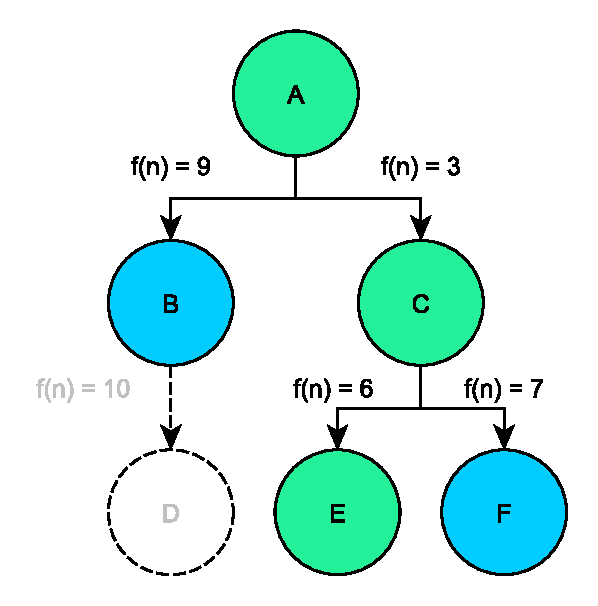
\includegraphics[width=0.6\textwidth]{Suchalgorithmen/bfs suchbaum}
	\captionsetup{justification=justified, format=plain}
  \caption{Suchbeispiel \"{u}ber Bestensuche}
  \label{fig:bestensuche beispiel}
\end{figure}


\begin{lstlisting}[language=Pseudo, caption={Pseudocode: Bestensuche}, mathescape=true, label={lst:pseudo bestensuche}]
FUNKTION bestensuche(Ausgangszustand) $\rightarrow$ Zielknoten
    offenen Liste $\leftarrow$ Prioritäts-Warteschlange
    offenen Liste $\leftarrow$ Knoten mit Ausgangszustand hinzufuegen
    SOLANGE offene Liste nicht leer
        Expansions Knoten $\leftarrow$ aus offenen Liste lesen und ihn daraus entfernen
        WENN Expansions Knoten Ziel erfuellt DANN
            ZURÜCKGEBEN $\rightarrow$ Expansions Knoten
            ENDE bestensuche()
        ENDE WENN
        FUER JEDEN Kindknoten VON expandiere(Knoten)
            offenen Liste $\leftarrow$ Kindknoten hinzufuegen
        NAECHSTER Knoten
    ENDE SOLANGE
    ZURÜCKGEBEN $\rightarrow$ Kein Zielknoten gefunden
ENDE bestensuche()

FUNKTION expandiere(Knoten) $\rightarrow$ Kindknoten Array
    Kindknoten $\leftarrow$ Array
    s $\leftarrow$ Knoten Zustand speichern
    FUER JEDE Kante VON ACTION(s)
        Kindknoten $\leftarrow$ durch Kante generieren
        f(Kindknoten) in Kindknoten speichern
        Kindknoten Array $\leftarrow$ Kindknoten hinzufuegen
    NAECHSTE Kante
    ZURÜCKGEBEN $\rightarrow$ Kindknoten Array
ENDE expandiere()
\end{lstlisting}

\subsection{A* Algorithmus}
\label{chap:a stern suchalgorithmus}

Der A* Algorithmus geh\"{o}rt zu den informierten und heuristischen Suchverfahren und ist eine Form der Bestensuche. Er ist ein vollst\"{a}ndiger Algorithmus, was bedeutet, dass er einen Pfad zu dem Ziel und findet, wenn einer vorhanden ist. Der A*-Algorithmus wird h\"{a}ufig in Routenplanern eingesetzt. Unter anderem benutzten, Game-Engines wie Godot 4.3 den A*-Algorithmus f\"{u}r die Navigation von NPCs.

\subsubsection{Bewertungsfunktion}
\label{chap:a stern bewertungsfunktion}

Bestensuchen benutzen eine Bewertungsfunktion $f(n)$, die dazu dient die Priorit\"{a}t eines Knoten $n$ w\"{a}hrend der Suche zu bewerten. Bei der Bewertungsfunktion des A*-Algorithmus werden dabei alle Pfad-Kosten $g(n)$ vom Ausgangsknoten bis zu dem Knoten $n$ mit der Heuristik $h(n)$ des Knoten $n$ summiert.


\begin{align}
	f(n) = g(n) + h(n)
\end{align}


Mit jeder Erweiterung des Pfades von $n$ zu $n^{\ast}$ steigen die Kosten $g(n)$. Dies liegt an den positiven Aktion-Kosten \textit{ACTIONCOST}$(n,a,n^*)$ der Kanten zwischen den Knoten.


\begin{align}
	g(n) + \textit{ACTIONCOST}(n,a,n^*) + h(n^*) &= g(n^*) + h(n^*)
\end{align}

\subsubsection{Heuristik}

Ein Suchalgorithmus sollte einen Pfad mit m\"{o}glichst geringen Kosten zum Ziel finden, der als optimaler Pfad bezeichnet wird. Ob der A*-Algorithmus einen optimalen Pfad findet, h\"{a}ngt von den Eigenschaften der Heuristik $h(n)$ ab. Eine Heuristik weist die Eigenschaften der Zul\"{a}ssigkeit und Konsistenz auf. Bei einer zul\"{a}ssigen Heuristik werden die Kosten stets untersch\"{a}tzt oder genau gesch\"{a}tzt. Die Kosten einer solchen Heuristik bleiben stets im Intervall $[0, h^{\ast}(n)]$ der tats\"{a}chlichen Kosten des Zielknoten $h^{\ast}(n)$.

\begin{align}
			0 \leq h(n) \leq h^*(n)
\end{align}

Eine konsistente Heuristik, muss gleichzeitig zul\"{a}ssig sein und die Dreiecksungleichung erf\"{u}llen. Umgekehrt muss eine zul\"{a}ssige Heuristik nicht konsistent sein. Die Dreiecksungleichung gibt an, dass die Heuristik $h(n)$ geringer sein soll als die Summe der Aktion $a$ und die Heuristik des folgenden Knoten $h(n^*)$.


\begin{align}
	h(n) \leq \textit{ACTIONCOST}(n,a,n^*) + h(n^*)
\end{align}

Die konsistente Heuristik weist eine st\"{a}rkere Eigenschaft auf, als eine zul\"{a}ssige Heuristik. Der expandierte Knoten bei einer konsistenten Heuristik wird optimal sein, weshalb dieser Knoten nicht erneut in die offene-Liste hinzuf\"{u}gt werden muss.

Bei einer inkonsistenten Heuristik k\"{o}nnen Pfade auftreten, die zu dem selben Zustand f\"{u}hren. Dies f\"{u}hrt dazu, dass mehrere Pfade mit demselben Zustand, aber unterschiedlichen Kosten, in der offenen Liste erscheinen, was zu h\"{o}heren Zeit- und Speicherkosten f\"{u}hrt.

\subsubsection{Beweis f\"{u}r Optimalit\"{a}t}
\label{chap:a stern be}

Arbeitet der A*-Algorithmus mit einer zul\"{a}ssigen oder konsistenten Heuristik, so wird diese den optimalen, kosteng\"{u}nstigsten Pfad zu einem Ziel finden.

Vorraussetzung:
\begin{itemize}
\item Der A*-Algorithmus expandiert auf Knoten mit der geringsten $f(n)$
\item Wir haben zwei m\"{o}gliche Zielknoten:
\begin{itemize}
	\item optimaler Zielknoten: $G_o$
	\item suboptimaler Zielknoten: $G_s_o$
\end{itemize}
\item Eine zul\"{a}ssige Heuristik: $0 \leq h(n) \leq h^*(n)$
\item Einen nicht expandierten Knoten: $n$
\end{itemize}

Beweis:
\begin{enumerate}
	\item Da keine weiteren Schritte vom Zielzustand m\"{o}glich sind gilt: $h(G_o) \land h(G_s_o) = 0$

		\begin{align}
			f(G_o) &= g(G_o) + h(G_o) \\
			f(G_o) &= g(G_o) \\
			f(G_s_o) &= g(G_s_o) + h(G_s_o) \\
			f(G_s_o) &= g(G_s_o)
		\end{align}

	
	Da $G_s_$ suboptimal ist folgt, dass die Pfadkosten $f(n)$ von $G_s_o > G_o$ sind und somit: $f(G_s_o) > f(G_o)$.
	\item Da $g(G_o)$ der tats\"{a}chliche Zielknoten ist und $h^*(n)$ die tats\"{a}chlichen Kosten von $G_o$ sind gilt:
    \begin{align}
			f(n) = g(n) + h(n) &< g(n) + h^*(n) = g(G_o) = f(G_o) \\
			f(n) &< g(G_o)
		\end{align}
\end{enumerate}
Aus 1. und 2. folgt: $f(n) < f(G_o) < f(G_s_o)$. Somit w\"{u}rde der A*-Algorithmus nicht zu $G_s_o$ f\"{u}hren und ist mit einer zul\"{a}ssigen Heuristik optimal.
\chapter{Goal Oriented Action Planning}
\label{chap:goap}

Das folgende Kapitel wird Goal Oriented Action Planning beschreiben. Es gehört zu den \hyperref[chap:entscheidungssysteme]{Entscheidungssystemen} in der Game-AI und besteht aus dem A* Suchalgorithmus. Es ist für die Planung an Aktionen zu einem bestimmten Ziel gedacht. Planung ist der Prozess der Suche einer Sequenz an Aktionen zur Erreichung eines Zieles. Die Suche kann dabei als Suchproblem dargestellt werden und durch Suchalgorithmen gelöst werden. Für das Verständnis wird daher Kenntnis der Themen Suchalgorithmen und Suchprobleme\ref{} empfohlen.

%ergänzen:
%\autocite{ai_standard}
%- Many NPCs nowadays remain hard-coded with little or no room for planning and adaptability. Goals in GOAP are not created with hard-coded plans but instead are dynamically replanned to react to environmental changes
%- GOAP offeers a more elegant structure that minimises code writing and maintenance. \autocite{}
%- As well, the debugging process is simpli ed, with GOAP providing the guarantee of valid plans, while hard coded plans may contain mistakes.
%- Code reusability is also encouraged with di erent NPCs being assigned to character types that share similar behaviour patterns
%- Each planning problem involves an iterative process in which small amounts of processor time are granted for computation, until a solution is found.
%- A number of issues still need to be addressed, such as the possible inclusion of hierarchical planning, and the potential integration of GOAP with scripting 
%- With real-time planning, some complex planning problems will require a substantial amount of processing time. This can be a drawback with current games allocating only 10percent of the processing time to AI
%- As well, the complexity of formulating a plan will increase as the number of actions and preconditions on actions grows, requiring even more processing power and time. Finally, implementing the GOAP architecture from scratch involves a considerable amount of time that game studios are not willing to spend.

\section{Historie}
\label{chap:goap historie}

Das \hyperref[chap:entscheidungssysteme]{Entscheidungssystem} \textit{Goal Oriented Action Planning} (\textit{GOAP}) entstand in der Entwicklung des Videospiel \textit{F.E.A.R First Encounter Assault Recon (2005)} durch das Entwicklerstudio \textit{Monolith}. Die Entwickler wollten ein Videospiel entwickeln, das wie ein Actionfilm wirkt, mit intensiven Kämpfen. Für die intensiven Kämpfe benötigt man NPC, welche Deckung nehmen, blind feuern, über Fenster springen, Granaten werfen, untereinander kommunizieren und weitere Aktionen ausführen können.

Zuvor nutzte \textit{Monolith} Finite State Machines (\textit{FSM}) als Entscheidungssystem. Den Entwicklern fiel es jedoch zunehmend aufwendig, eine FSM mit neuen Zuständen und den dazugehörigen Aktionen zu erweitern. In einem vorherigen Videospiel \textit{No One Lives Forever (2000)}, wurde veruscht eine dynamische FSM zu implementieren, die sich an Zielzustände anpassen konnte. Allerdings wurde auch diese Lösung als zu unflexibel wahrgenommen. Aus dem Versuch der dynamischen FSM und STRIPS hat Jeff Orkin das GOAP System entwickelt, welches Echtzeitplanung erfüllen soll. Eine der Herausforderungen, mit denen sich Jeff Orkin während der Entwicklung konfrontiert sah, war die Berücksichtigung der Performance.\autocite{retro_fear}



\section{GOAP Bestandteile}
\label{chap:goap bestandteile}

Das GOAP -System basiert dabei auf dem STRIPS System. Wie auch STRIPS besitzt GOAP Ziele, welche einen gewünschten Zustand beschreiben und Goap-Aktion mit Effekten die Zustände ändern können. GOAP sucht nach einer Sequenz an Goap-Aktion, der Aktions-Sequenz, die das Ziel des NPC erreichen kann. Im Sinne von Jeff Orkins geschieht die eigentliche Ausführung der Aktionen über eine Finite State Machine (\textit{FSM}).


\subsection{Finite State Machine in GOAP}
\label{chap:fsm goap}

Das Videospiel \textit{F.E.A.R} benötigt für die Ausführung der Aktionen eine FSM. Die NPCs führen ihre Aktionen durch eine Kombination aus Animationen und Bewegungen aus. Beispielsweise sorgt eine Cover-Aktion dafür, dass der NPC hinter eine Deckung läuft und dort eine Deckungs-Animation abspielt. Eine Shoot-Aktion hingegen aktiviert eine entsprechende Schuss-Animation. Die FSM besteht dabei aus den drei Zuständen GoTo, Animate und UseSmartObject. 
\begin{figure}[h]
  \centering
  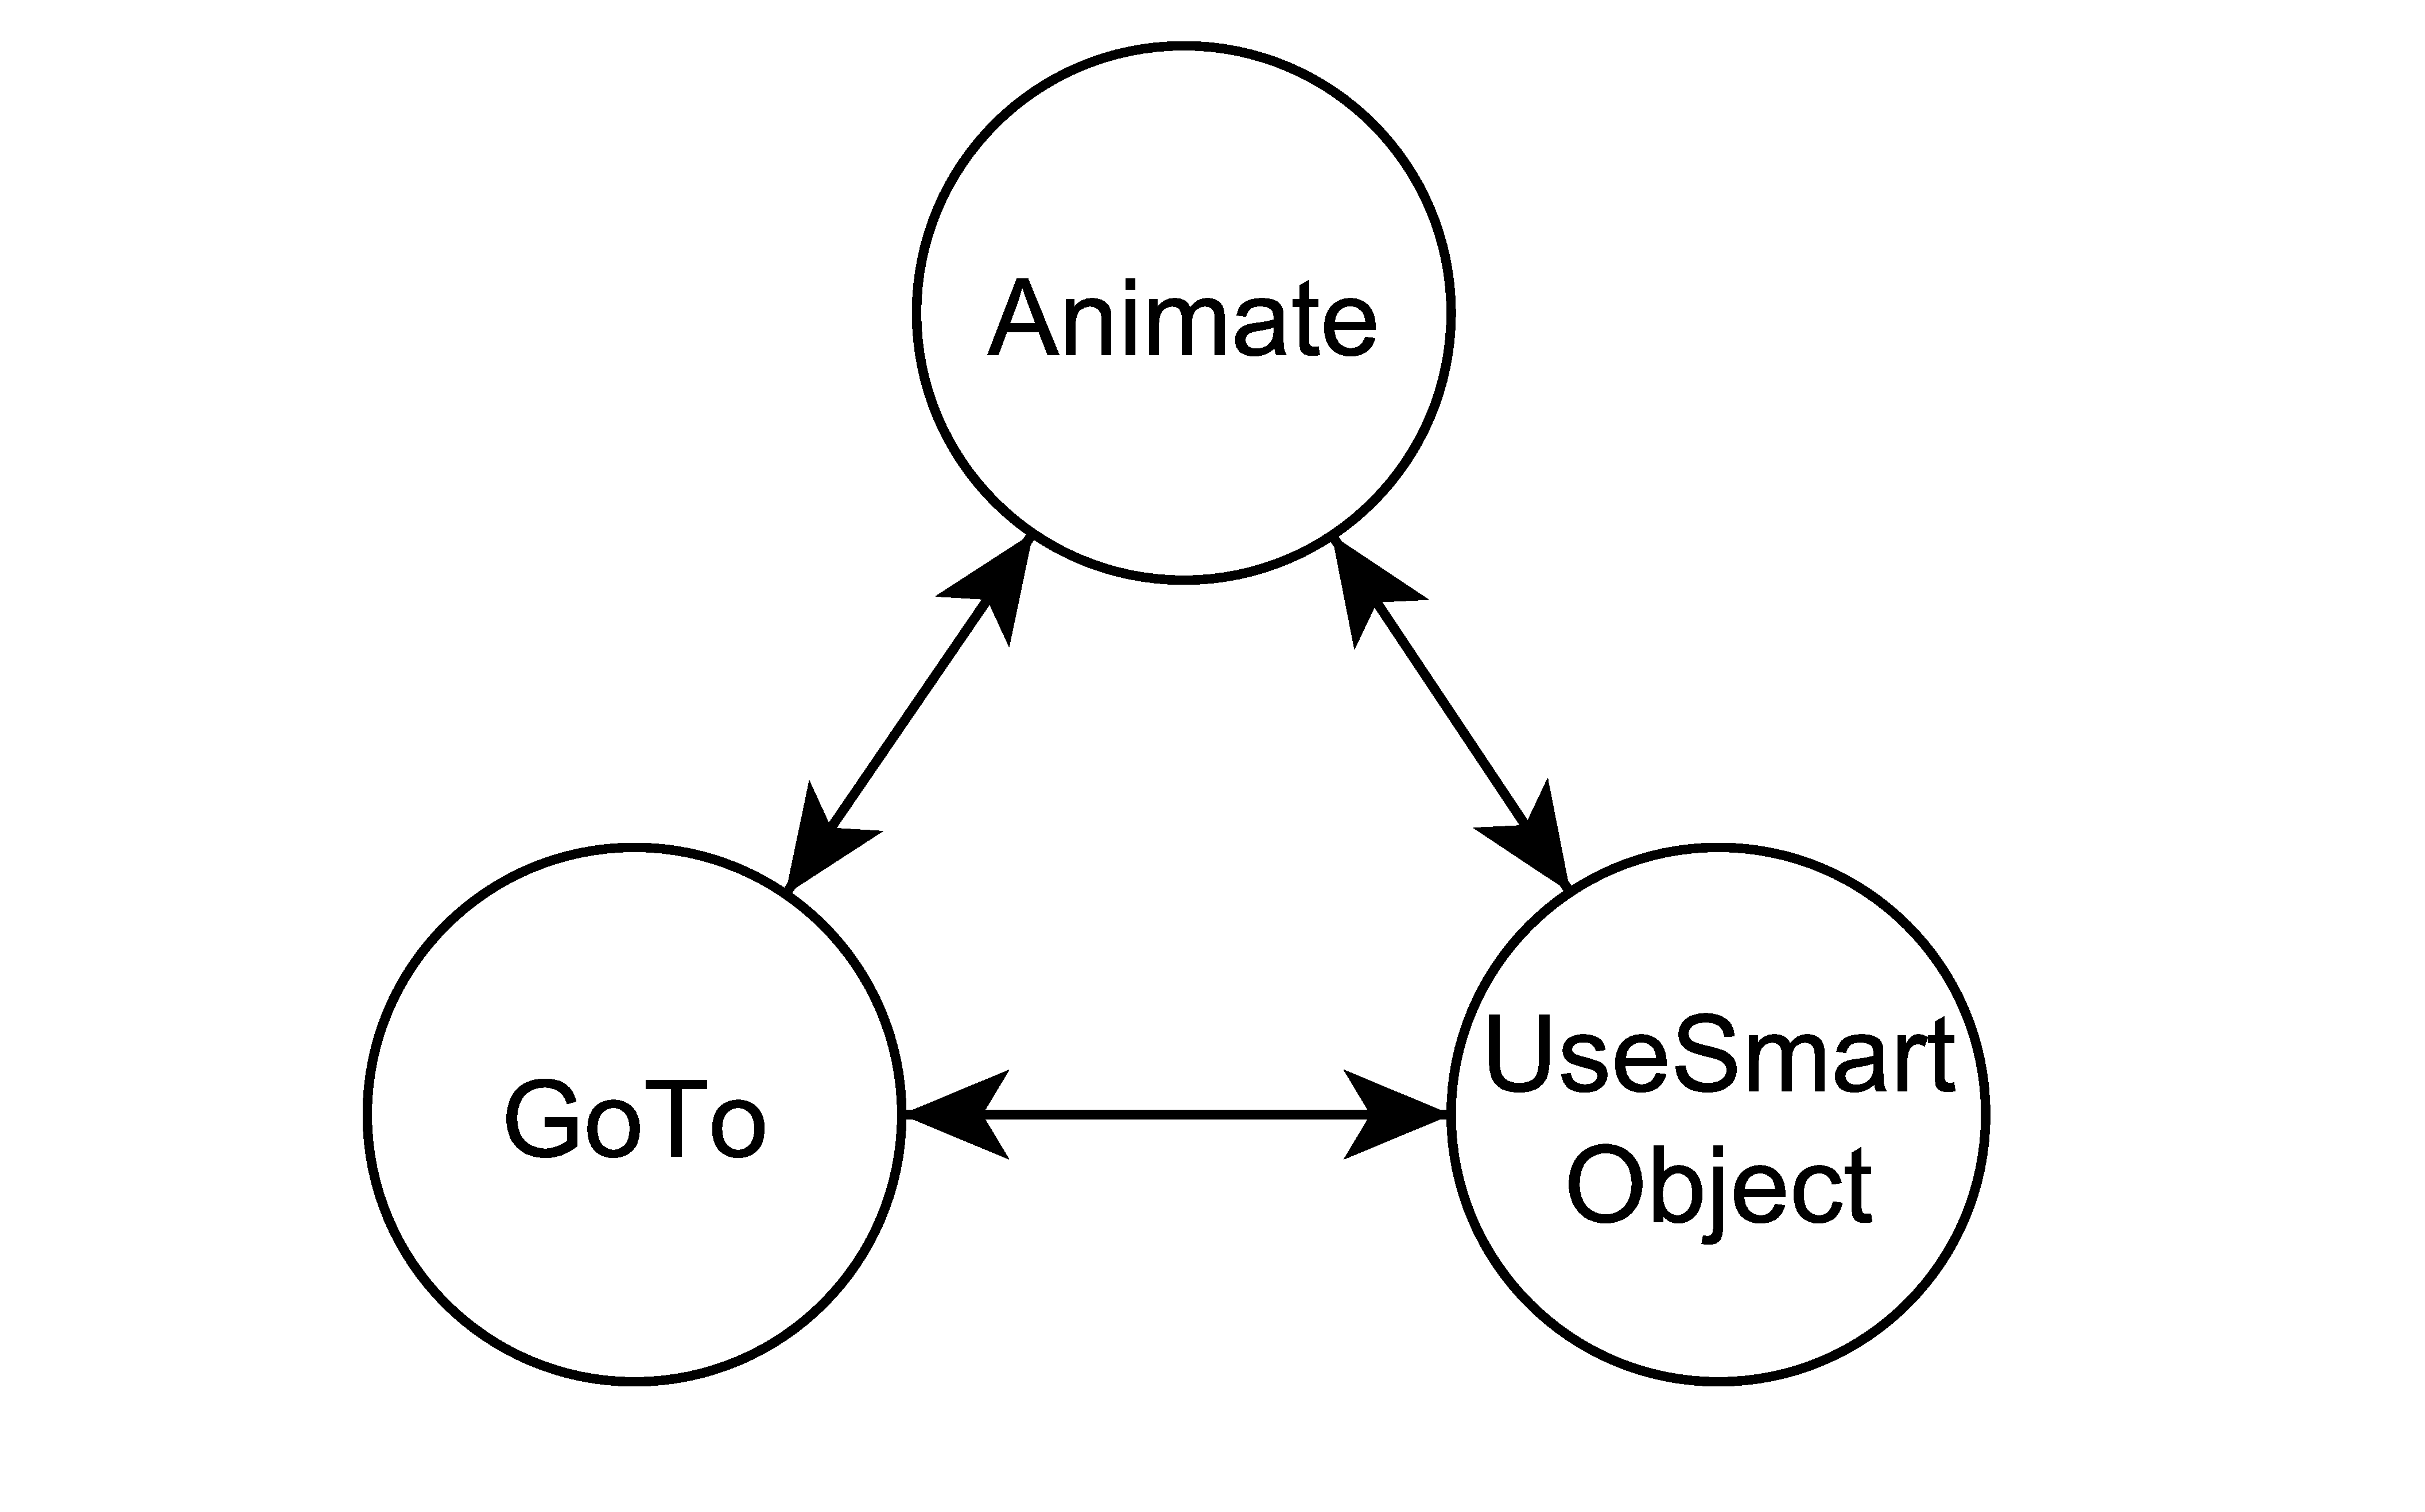
\includegraphics[width=0.7\textwidth]{GOAP/fsm.pdf}
	\captionsetup{justification=justified, format=plain}
  \caption{GOAP Finite State Machine}
  \label{fig:Goap FSM}
\end{figure}

\textit{Monolith} hat durch die Zustände \textit{Animate} und \textit{UseSmartObject} Animationen umgesetzt. Der Unterschied zwischen den beiden Zuständen besteht darin, dass \textit{UseSmartObject} Animationen steuert, die von \textit{SmartObjects} in der Spielwelt vorgegeben werden, während \textit{Animate} Animationen abspielt, die direkt im NPC gespeichert sind. Der Zustand \textit{GoTo} hat ebenfalls Animationen abgespielt, kombiniert diese jedoch mit der tatsächlichen Bewegung des NPCs durch die Spielwelt.

Die Zustandswechsel werden durch die Goap-Aktion bestimmt, welche wiederum durch GOAP gegeben werden.


\subsection{GOAP Ziele}
\label{chap:goap ziele}

Ein Ziel $GOAL(g)$ in GOAP setzt die erwünschte Zielzustände für den Planer. So setzt das Ziel $EliminatePlayer$ den Zielzustand $\{\lnot PlayerAlive\}$.
\[
	\highlightbox{0.9\textwidth}{$
		\begin{align*}
			GOAL(EliminatePlayer) = \{\lnot PlayerAlive\}
		\end{align*}
	$}
\]

Die Auswahl des Zieles geschieht nach ihrer Priorität und ob dieses gültig ist. Das Ziel mit der höchsten Priorität und Gültigkeit wird bevorzugt. Die Gültigkeit und Priorität basiert dabei auf dem Zustand $s$ des NPC und seiner Umwelt. So ist das Ziel $EliminatePlayer$ mit dem Zustand $s$ nicht gültigt und besitzt eine hohe Priorität.
\[
	\highlightbox{0.9\textwidth}{$
		\begin{align*}
			s = \{\lnot PlayerVisible\} \\
			PRIORITY(s,EliminatePlayer) = 100 \\
			VALID(s,EliminatePlayer) = false
		\end{align*}
	$}
\]


\subsection{GOAP Aktionen}
\label{chap:goap actions}

Die Goap-Aktion können Weltzustände oder auch direkte Zustände eines NPC ändern. So kann beispielsweise die Goap-Aktion \textit{Reload} den Zustand $s = \{\lnot GunLoaded\}$ mit seinem Effekt ändern.
\[
	\highlightbox{0.9\textwidth}{$
		\begin{align*}
			TRANSITIONS(s,Reload) &= \{GunLoaded\}
		\end{align*}
	$}
\]

Dadurch haben Goap-Aktion die Möglichkeit Zielzustände zu erreichen. Man nehme an, dass der NPC das Ziel $Patrol$ verfolgt, mit dem gewünschten Zustand $AtPatrol$, und dass die Aktion $GoPatrol$ den Effekt $TRANSITIONS(s, GoPatrol) = {AtPatrol}$ hat. In diesem Fall kann die Goap-Aktion durch ihren Effekt den gewünschten Zielzustand erreichen.

Eine Goap-Aktion hat auch Vorbedingungen als Zustände, diese Zustände können wiederum von anderen Goap-Aktionen erfüllt werden. So kann beispielsweise die Goap-Aktion $Reload$ die Vorbedingung der Goap-Aktion $Shoot$ erreichen.
\[
	\highlightbox{0.9\textwidth}{$
		\begin{align*}
			PRECONDITION(Shoot) = \{GunLoaded\}
		\end{align*}
	$}
\]

Eine Goap-Aktion setzt auch wie im Suchproblem\ref{} eine $ACTIONCOST$ Funktion um, die später zur Auswahl einer Goap-Aktion herangezogen wird. Wird die Goap-Aktion ausgewählt wird diese später von der FSM ausgeführt.


\subsubsection{Fallbeispiel}
\label{chap:goap action beispiel}

Nehmen wir an, dass der NPC den Ausgangszustand $s_a$ und das Ziel $EliminatePlayer$ besitzt.
\[
	\highlightbox{0.9\textwidth}{$
		\begin{align*}
			s_a = \{PlayerVisible, \lnot GunLoaded\, \lnot AtCover\} \\
			GOAL(EliminatePlayer) = \{\lnot PlayerAlive\}
		\end{align*}
	$}
\]

Der NPC muss nun versuchen das Ziel mit den möglichen Goap-Aktion den Zielzustand $\{\lnot PlayerAlive\}$ erreichen. Die möglichen Goap-Aktion werden dafür aus einer $ACTIONS(s)$ Funktion gelesen.
\[
	\highlightbox{0.9\textwidth}{$
		\begin{align*}
			ACTIONS(s) = \{Reload, MoveToCover\} \\
			TRANSITIONS(s,Reload) = \{GunLoaded\} \\
			TRANSITIONS(s,MoveToCover) = \{AtCover\}
		\end{align*}
	$}
\]

Aus der $TRANSITIONS$ Funktion können wir entnehmen, dass keine der Goap-Aktion den Zustand $\lnot PlayerAlive$ direkt erreichen kann. Es muss ein Zustand entdeckt werden aus dem mit einer entsprechenden Goap-Aktion das Ziel erreicht werden kann. Eine Lösung wäre \textit{Brute Force}, das durchgehen aller möglichen Goap-Aktion bis letztlich das Ziel gefunden wird. Dies sorgt jedoch für einen hohen Rechenaufwand bei komplexen NPC mit vielen Goap-Aktion und Zuständen. Außerdem können beim Brute Force suboptimale Aktions-Sequenzen gefunden werden, da dieser die Kosten der Goap-Aktion nicht beachtet. In GOAP sucht der A*-Suchalgorithmus über den GOAP Planner die optimale Aktions-Sequenz.


\subsection{GOAP Planner}
\label{chap:goap planner}

Der GOAP Planner ist dabei die eigentliche Lösung des Suchproblems. Der Planner bestimmt das Ziel mit der höchsten Priorität und Gültigkeit. Die dazugehörige Aktions-Sequenz wird über den A*-Suchalgorithmus im GOAP Planner gesucht. Der A*-Suchalgorithmus\ref{} wird im Kapitel Suchalgorithmen ausführlich beschrieben.

\subsubsection{Knoten und Kanten}
\label{chap:goap knoten und kanten}

Der A*-Suchalgorithmus ist in der Videospiel-Entwicklung für die Suche des Navigation-Pfades bekannt. Er kann aber auch für andere Suchprobleme genutzt werden, wie für die Suche einer Aktion-Sequenz. Wie auch für die Navigation erzeugt der A*-Suchalgorithmus einen Suchbaum, mit dem Unterschied, dass die Knoten Zustände des NPC sind, die durch die Kanten also Goap-Aktionen erzeugt werden.

Knoten speichern die nicht erfüllten Zustände des NPC für das erreichen des Zieles ab, während Kanten die Goap-Aktionen darstellen die von einem Knoten zu einem neuen Knoten führen.

\begin{table}[h]
  \caption{A* Vergleich: Navigation und Aktions-Plannung}
  \label{A*: Vergleich}
  \renewcommand{\arraystretch}{1.2}
  \centering
  \small
    \begin{tabularx}{0.95\textwidth}{X X X}
      \toprule
      \textbf{A*} & \textbf{Navigation} & \textbf{Aktion-Plannung}\\
      \toprule
      Knoten & NavMesh Polygon & Zustand &
			Kanten & NavMesh Polygon Kanten & Goap-Aktionen &
      \bottomrule
    \end{tabularx}
\end{table}


\subsubsection{Bewertungsfunktion}
\label{chap:goap bewertungsfunktion}

Die Bewertungsfunktion des A*-Suchalgorithmus setzt sich aus $f(n) = g(n) + h(n)$ zusammen. In GOAP ist $g(n)$ die Funktion $ACTIONCOST(s,a,s^*)$, welche die Kosten der Kante darstellt, also die Kosten für die Ausführung der Goap-Aktion $a$, die vom Zustand $s$ zum Zielzustand $s^$ führt. Die Heuristik $h(n)$ wird durch die Summe der noch nicht erfüllten Zustände des jeweiligen Knotens dargestellt. Je geringer der Wert von $h(n)$, desto näher ist der Knoten dem Ziel. 


\subsubsection{Suche der Aktions-Sequenz}
\label{chap:goap suche}

Es ist zwar möglich aus dem Ausgangszustand zu suchen, könnte aber einem \textit{Brute Force}\ref{} ähneln und dadurch ineffizient sein. Die Kante wird nicht wie bei der Navigation vom Ausgangszustand ausgewählt, sondern aus dem Zielzustand $s_z$ aus. Von dort aus wird die Suche nach Kanten fortgesetzt, die die Vorbedingungen der zuvor gewählten Kante erfüllen. Die Suche wird fortgesetzt bis alle Vorbedingungen der Kanten erfüllt wurden. Der Planer speichert dabei die Auswahl der Goap-Aktionen in einer Aktions-Sequenz ab.


\section{Suchbeispiel}
\label{chap:goap suchbeispiel}

Wir setzten das Beispiel mit dem Wissen über den GOAP Planner fort. Dabei definiert $s_a$ den Ausgangszustand des NPC.
\[
	\highlightbox{0.9\textwidth}{$
		\begin{align*}
			s_a = \{PlayerAlive, PlayerVisible, \lnot AtPatrol, \lnot GunLoaded\, \\
			\lnot AtCover, \lnot AtPlayer,  \lnot AtLastPlayerPostion\}
		\end{align*}
	$}
\]


\subsubsection{Auswahl des Zieles}
\label{chap:goap ziel auswahl}

\begin{table}[h]
  \caption{Ziel Tabelle}
  \label{Kap4:Ziel}
  \renewcommand{\arraystretch}{1.2}
  \centering
  \small
    \begin{tabularx}{0.95\textwidth}{X X X R}
      \toprule
      \textbf{Goal} & \textbf{Ziel-Zustand} & \textbf{Gültigkeit} & \textbf{Priorität}\\
      \toprule
      EliminatePlayer & \lnot$ PlayerAlive & PlayerVisible & 3 \\
			SearchEnemy & AtLastPlayerPostion & \lnot AtLastPlayerPostion & 2 \\
			Patrol & \lnot$ AtPatrol & AtLastPlayerPostion & 1 &
      \bottomrule
    \end{tabularx}
\end{table}

Der GOAP Planer wählt das Ziel mit der höchsten Priorität und Gültigkeit. Nehmen wir an, dass das Ziel \textit{Patrol} aufgrund der \textit{VALID(s,Patrol)} Funktion nicht gültig ist, so würde das Ziel ausfallen. Es verbleiben die Ziele: \textit{EliminatePlayer} und \textit{SearchEnemy}. Da \textit{EliminatePlayer} mit $PRIORTIY(s,EliminatePlayer) = 3$ die höhere Priorität hat, wird diese als Ziel ausgewählt.

\subsubsection{Suche nach der Aktion-Sequenz}
\label{chap:goap suche nach aktionen}

\begin{table}[h]
  \caption{Aktionen ihre Effekte und Vorausgesetzte Zustände}
  \label{Kap4:Aktionen}
  \renewcommand{\arraystretch}{1.2}
  \centering
  \small
    \begin{tabularx}{0.95\textwidth}{l l l l}
      \toprule
      \textbf{Aktion} & \textbf{Effekt} & \textbf{Vorausgesetzte Zustände} & \textbf{Kosten}\\
      \toprule
      Shoot & \lnot$ PlayerAlive & GunLoaded, PlayerVisible & 1\\
			Melee & \lnot$ PlayerAlive & AtPlayer, PlayerVisible & 3\\
      Reload & GunLoaded & \lnot$ GunLoaded & 1\\
      GoTo & AtCover, AtPlayer, AtLastPlayerPostion & - & 0-10 &
      \bottomrule
    \end{tabularx}
\end{table}
$

Der Algorithmus erstellt nun einen Suchbaum. Der Wurzelknoten im Suchbaum speichert, dabei den erwünschten Zielzustand des Zieles. Im Falle des Beispiels ist der Zielzustand $s_z = GOAL(EliminatePlayer) = \{\lnot PlayerAlive\}$.

\begin{figure}[h]
  \centering
  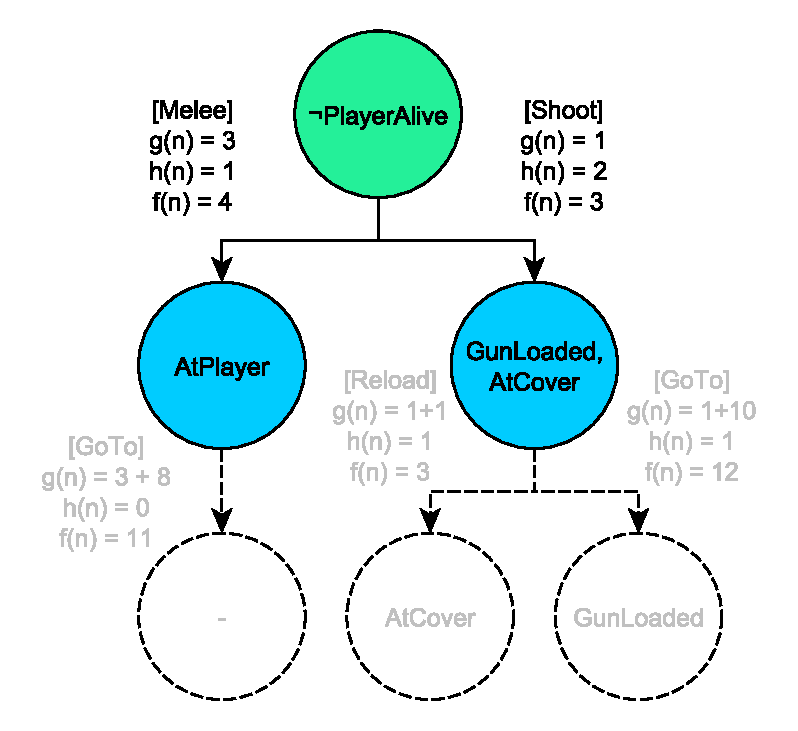
\includegraphics[width=0.5\textwidth]{GOAP/goap baum 1}
	\captionsetup{justification=justified, format=plain}
  \caption{GOAP A* Suche: Grüne Knoten sind Knoten, welche erweitert wurden. Blaue Knoten sind Knoten aus der offenen Liste.}
  \label{fig:goap1}
\end{figure}

Nun sucht der Planner alle möglichen Aktionen die den Zielzustand erreichen ($ACTIONS(s_z) = {Shoot, Melee}$). Es werden nicht erfüllte und vorausgesetzte Zustände der gefundenen Aktionen, sowie die Kosten $g(n)$ und $f(n)$ in den Knoten hinterlegt. Beide werden in die offene Liste hinzugefügt.

Zur weiteren Suche entscheidet sich der A* Algorithmus für den Knoten mit den geringsten Kosten aus der offenen Liste, welcher durch die Bewertungsfunktion $f(n) = g(n) + h(n)$ berechnet wurde. Die Kosten $g(n)$ werden durch die $ACTIONCOST$-Funktion gelesen. Die Heuristik $h(n)$ stellt sich durch die Summe an noch nicht erfüllten Zuständen. Im Beispiel expandiert A* den Knoten \textit{GunLoaded, AtCover} der durch die Aktion \textit{Shoot} generiert wurde. Der Zustand \textit{AtPlayer} bleibt weiterhin in der offenen Liste.

\begin{figure}[h]
  \centering
  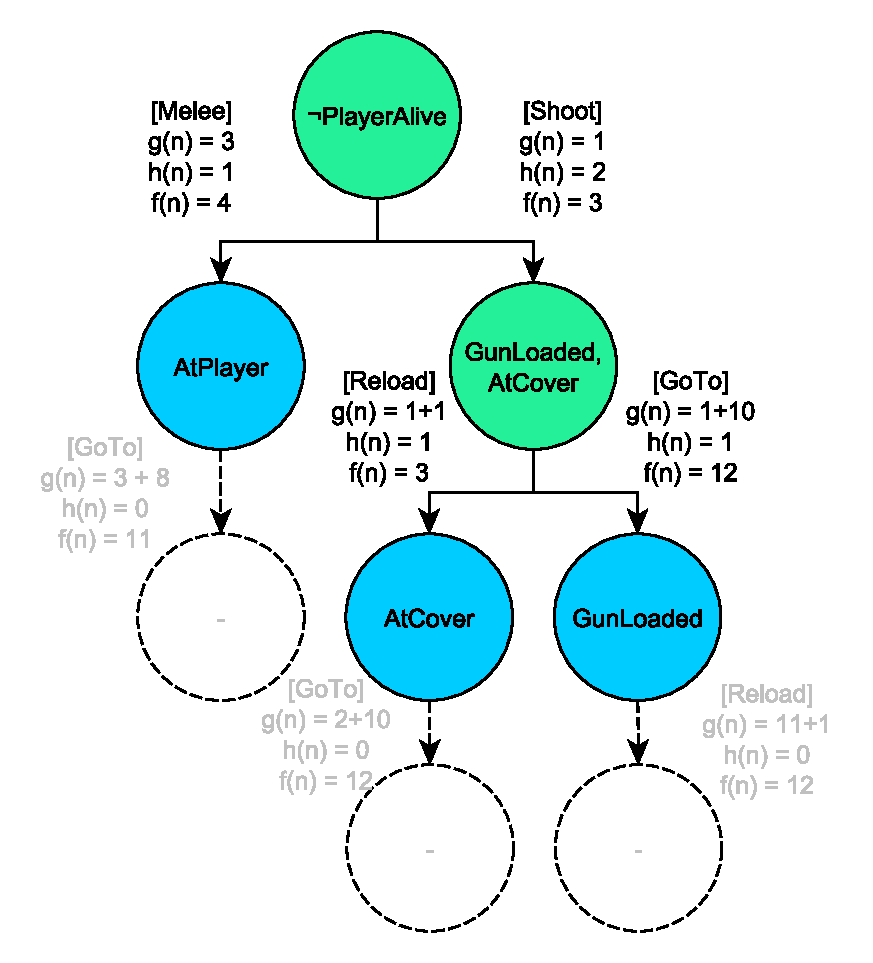
\includegraphics[width=0.6\textwidth]{GOAP/goap baum 2}
	\captionsetup{justification=justified, format=plain}
  \caption{GOAP A* Suche}
  \label{fig:goap2}
\end{figure}

Für den expandierten Knoten \textit{GunLoaded, AtCover} werden nun Aktionen gesucht, die die Zustände des Knoten erfüllen. In dem Beispiel sind es \textit{Reload} und \textit{GoTo}. Auch die Knoten die durch die Aktionen entstehen, werden in die offene Liste hinzugefügt. Erneut wählt A* den Knoten mit den geringsten Kosten $f(n)$ zur Expansion.
\clearpage

\begin{figure}[h]
  \centering
  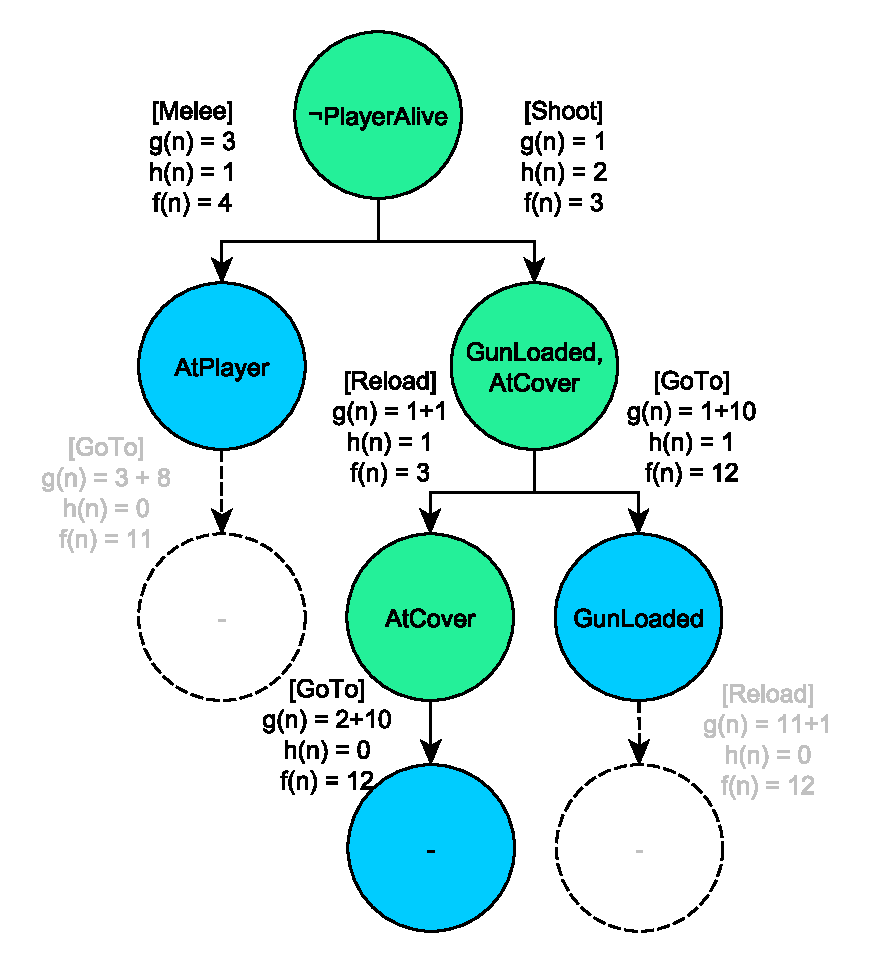
\includegraphics[width=0.6\textwidth]{GOAP/goap baum 3}
	\captionsetup{justification=justified, format=plain}
  \caption{GOAP A* Suche}
  \label{fig:goap3}
\end{figure}

Der Knoten der durch die Aktion \textit{Reload} entstand, hat dabei die geringsten $f(n)$ Kosten. Der nachfolgende Knoten, der durch die Aktion \textit{GoTo} erzeugt wird, hat zwar einen leeren Zustand und wäre somit abgeschlossen, befindet sich jedoch gemeinsam mit dem \textit{AtPlayer}-Knoten, der geringere Kosten hat, noch in der offenen Liste.

\begin{figure}[h]
  \centering
  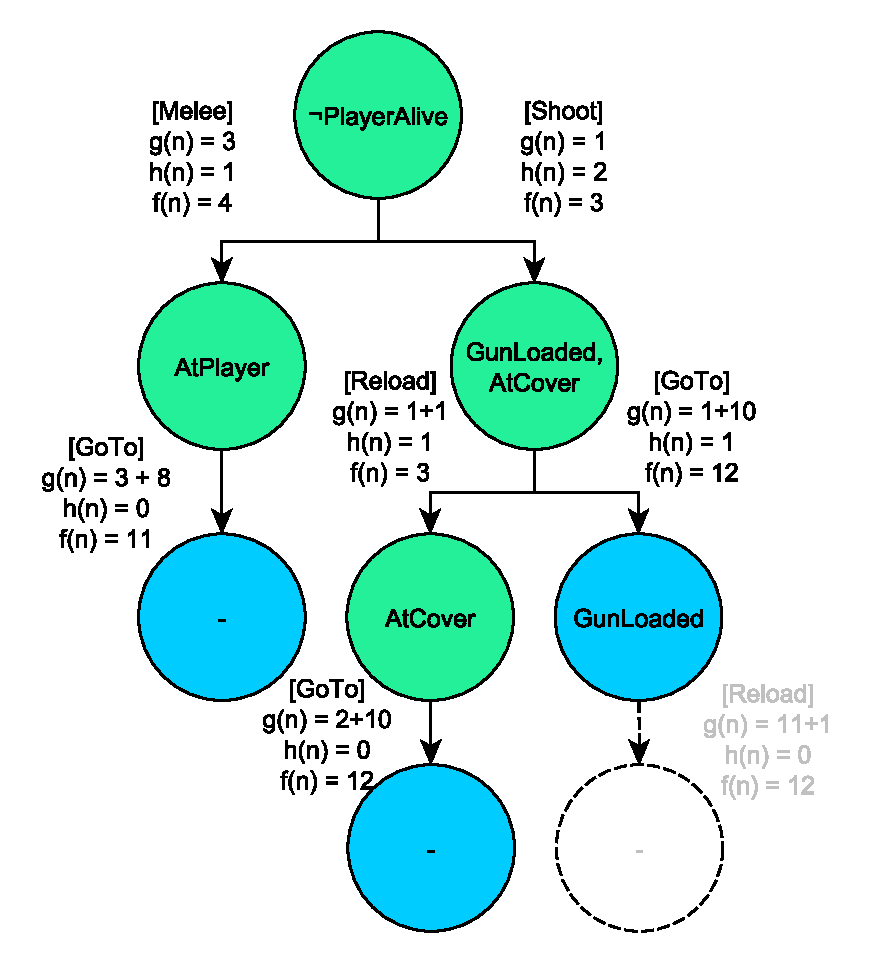
\includegraphics[width=0.6\textwidth]{GOAP/goap baum 4}
	\captionsetup{justification=justified, format=plain}
  \caption{GOAP A* Suche}
  \label{fig:goap4}
\end{figure}

Aus der offenen Liste wird der nächste Knoten mit dem Zustand \textit{AtPlayer} gewählt, da dieser die niedrigsten Kosten von allen anderen offenen Knoten hat. Dieser wird durch die Aktion \textit{GoToPlayer} erfüllt und führt zu einem Knoten mit leerem Zustand.

\begin{figure}[h]
  \centering
  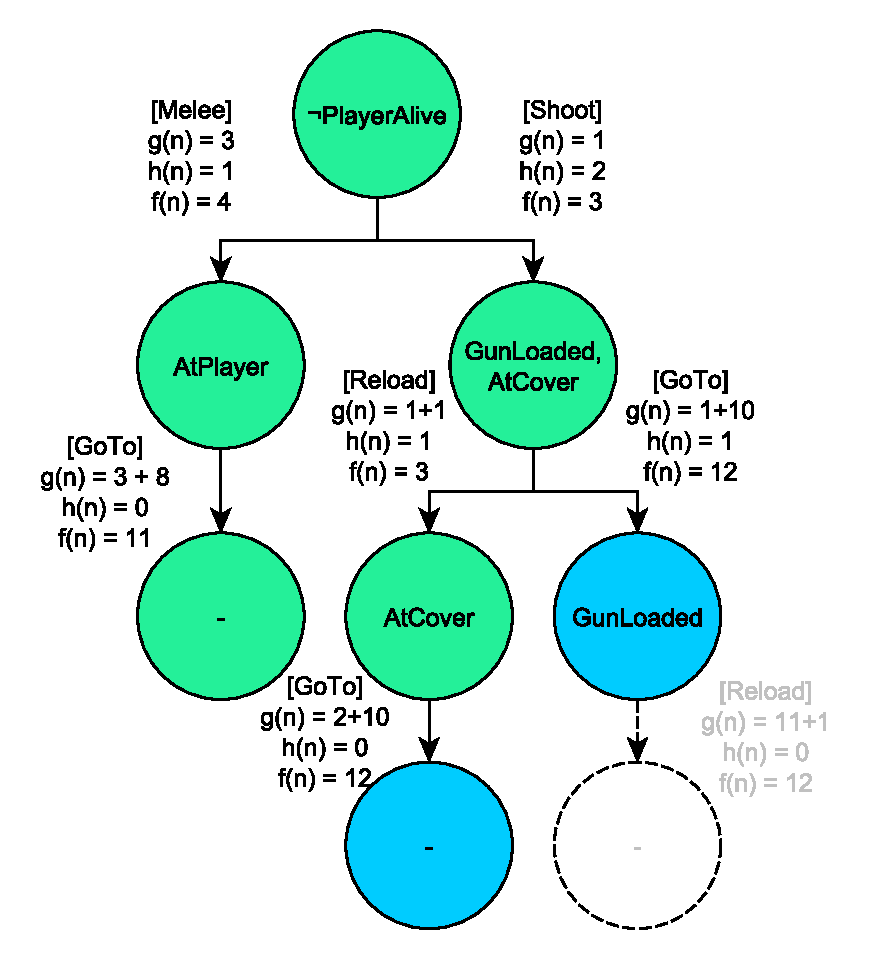
\includegraphics[width=0.6\textwidth]{GOAP/goap baum final}
	\captionsetup{justification=justified, format=plain}
  \caption{GOAP A* Suche}
  \label{fig:goap5}
\end{figure}

Letztlich wird der günstigste Knoten aus der offenen Liste genommen. Da dieser erfüllt ist, beziehungsweise keine weiteren Zustände besitzt, gibt der Planner nun die Goap-Aktionen, also die Kanten, die zu ihm geführt habe in einer Aktions-Sequenz zurück. Im Beispiel wäre es die Aktions-Sequenz: [\textit{Melee, GoTo}]. Diese Aktions-Sequenz muss nun gespiegelt werden, da der A*-Suchalgorithmus vom Zielzustand angefangen hat. Somit wäre die richtige Aktions-Sequenz: [\textit{GoToPlayer, Melee}].
\chapter{State of the art}



\section{Videospiel-Markt}

Videospiele sind Bestandteil des Medienkonsums in Deutschland. Rund 6 von 10 Menschen in Deutschland spielen Computer- und Videospiele. Der deutsche Videospiel-Markt machte mit Videospiel-Hardware, Videospiel-Abo-Diensten und Videospielen im Jahr 2023 einen Umsatz von 9,97 Milliarden Euro. Dabei machten Videospiele und In-Game K�ufe mit 5,845 Milliarden Euro einen Umsatz von ca. 59\% aus. Im Vorjahr 2022 entstand ein Umsatz von 9,432 Milliarden Euro, somit stieg der Umsatz von 2022 im Jahr 2023 um 6\%.  Zahlen f�r das Jahr 2024 sind noch nicht bekannt.

\begin{figure}[h]
  \centering
  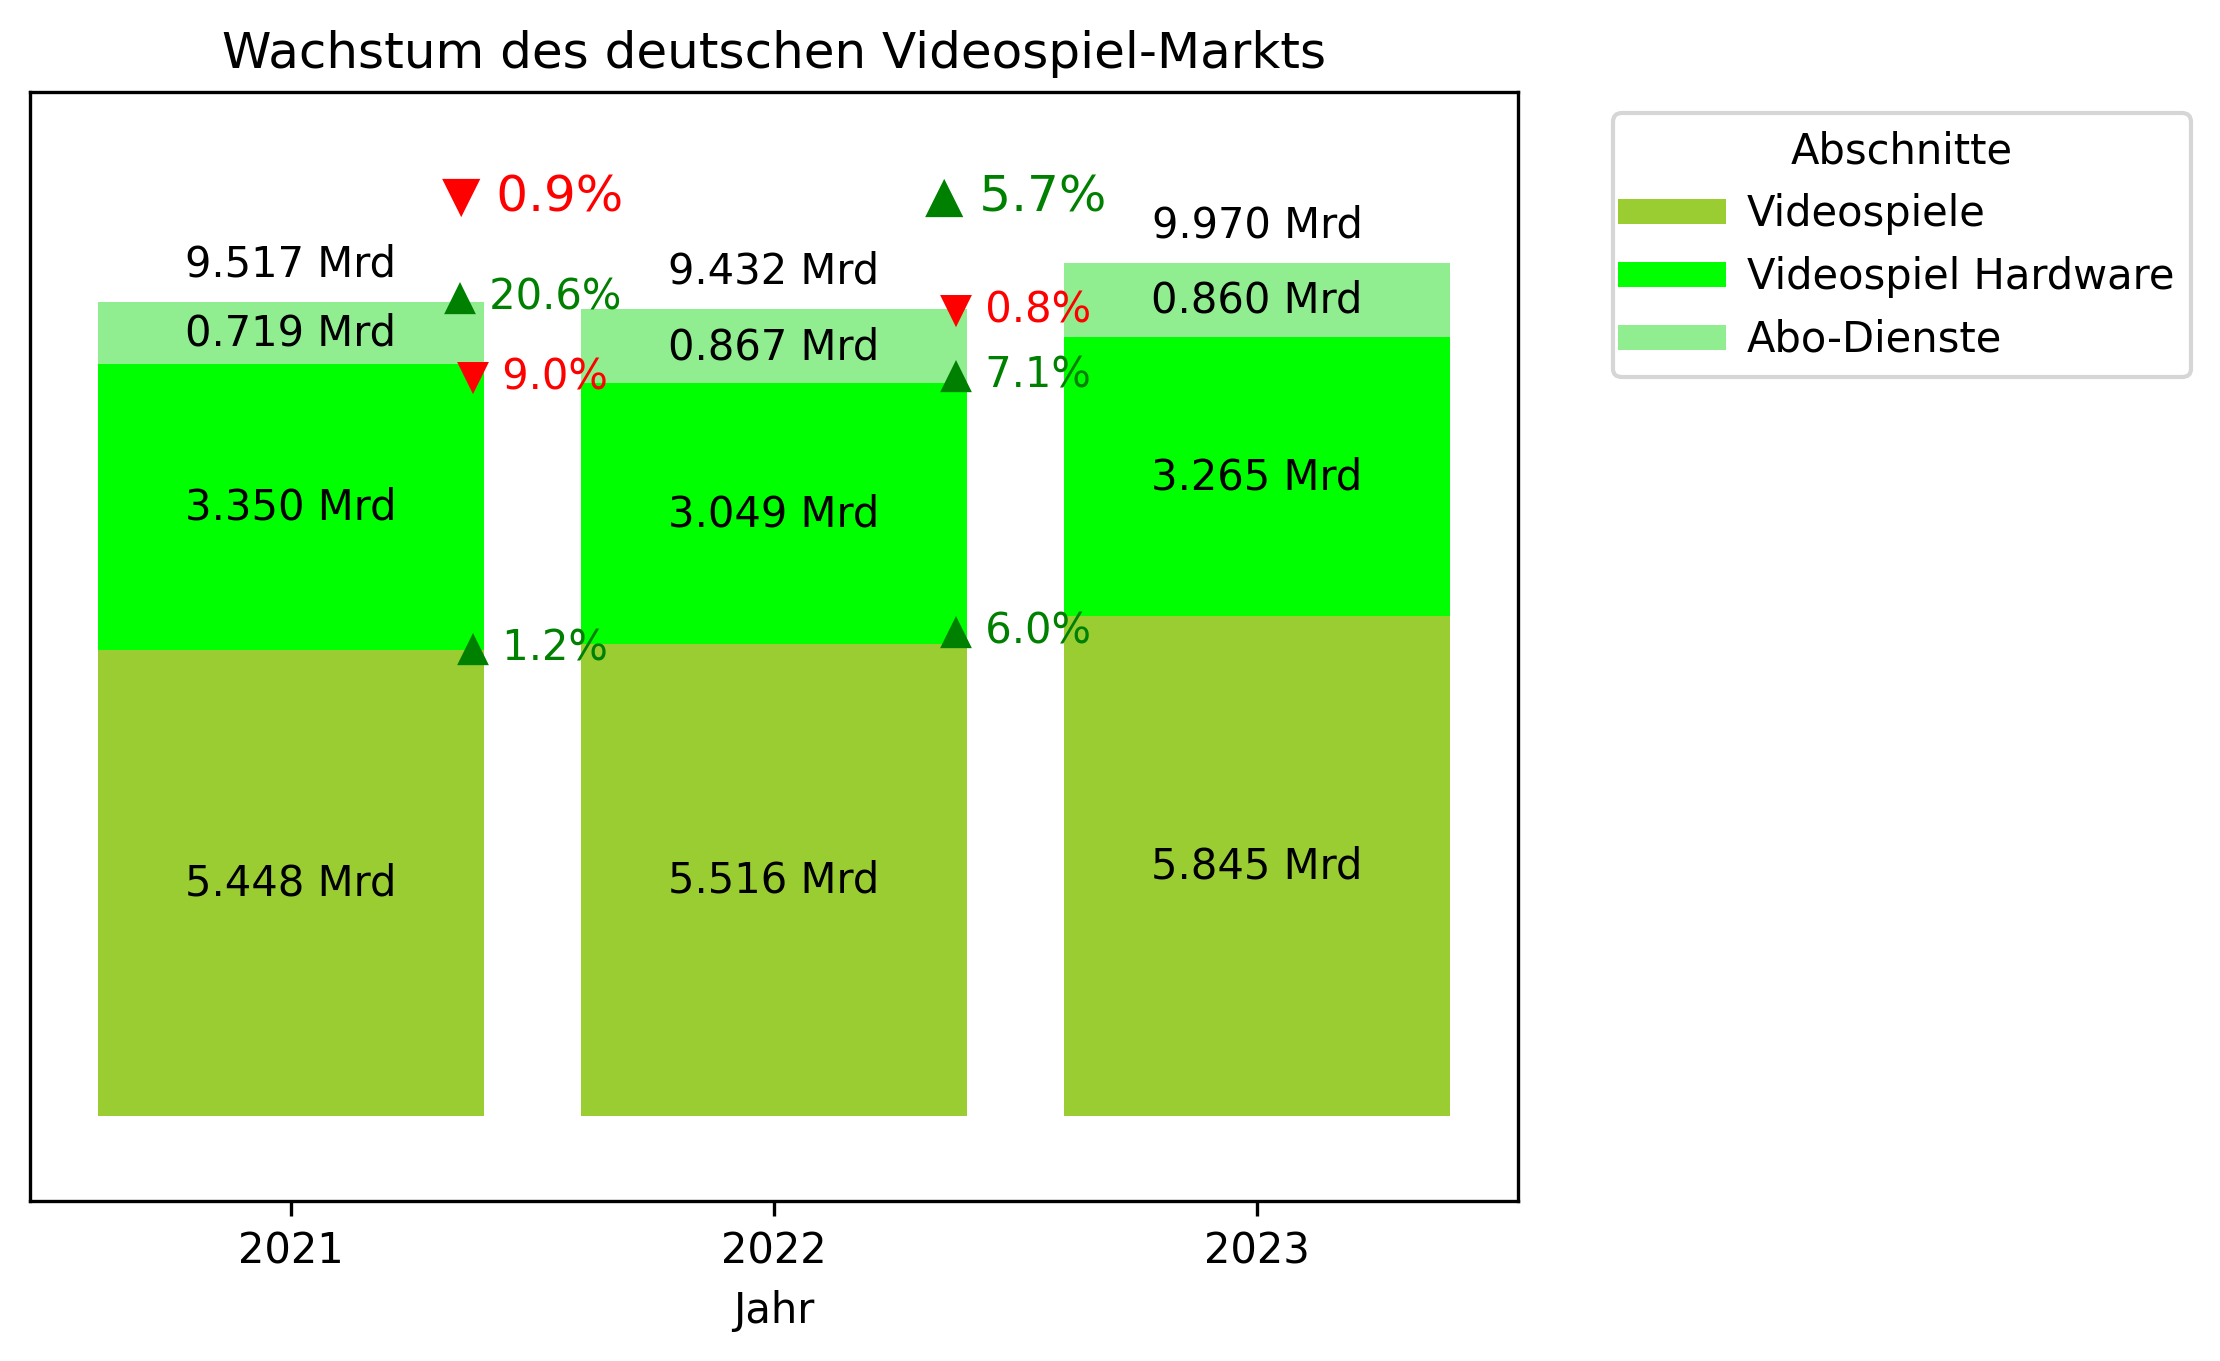
\includegraphics[width=15cm]{state_of_the_art/deutscher_vs_markt}
	\captionsetup{justification=justified, format=plain}
  \caption{Wachstum des deutschen Videospielmarkts �ber die Jahre}
  \label{Deutscher Videospielmarkt}
\end{figure}

Auf der erfolgreichen Computerspiel Vertriebsplattform Steam von Valve wurden vergangenes Jahr 2023 14.324 Computerspiele ver�ffentlicht. Seit 2019 w�chst die Ver�ffentlichung der Computerspiele auf Steam stetig.

\begin{figure}[h]
  \centering
  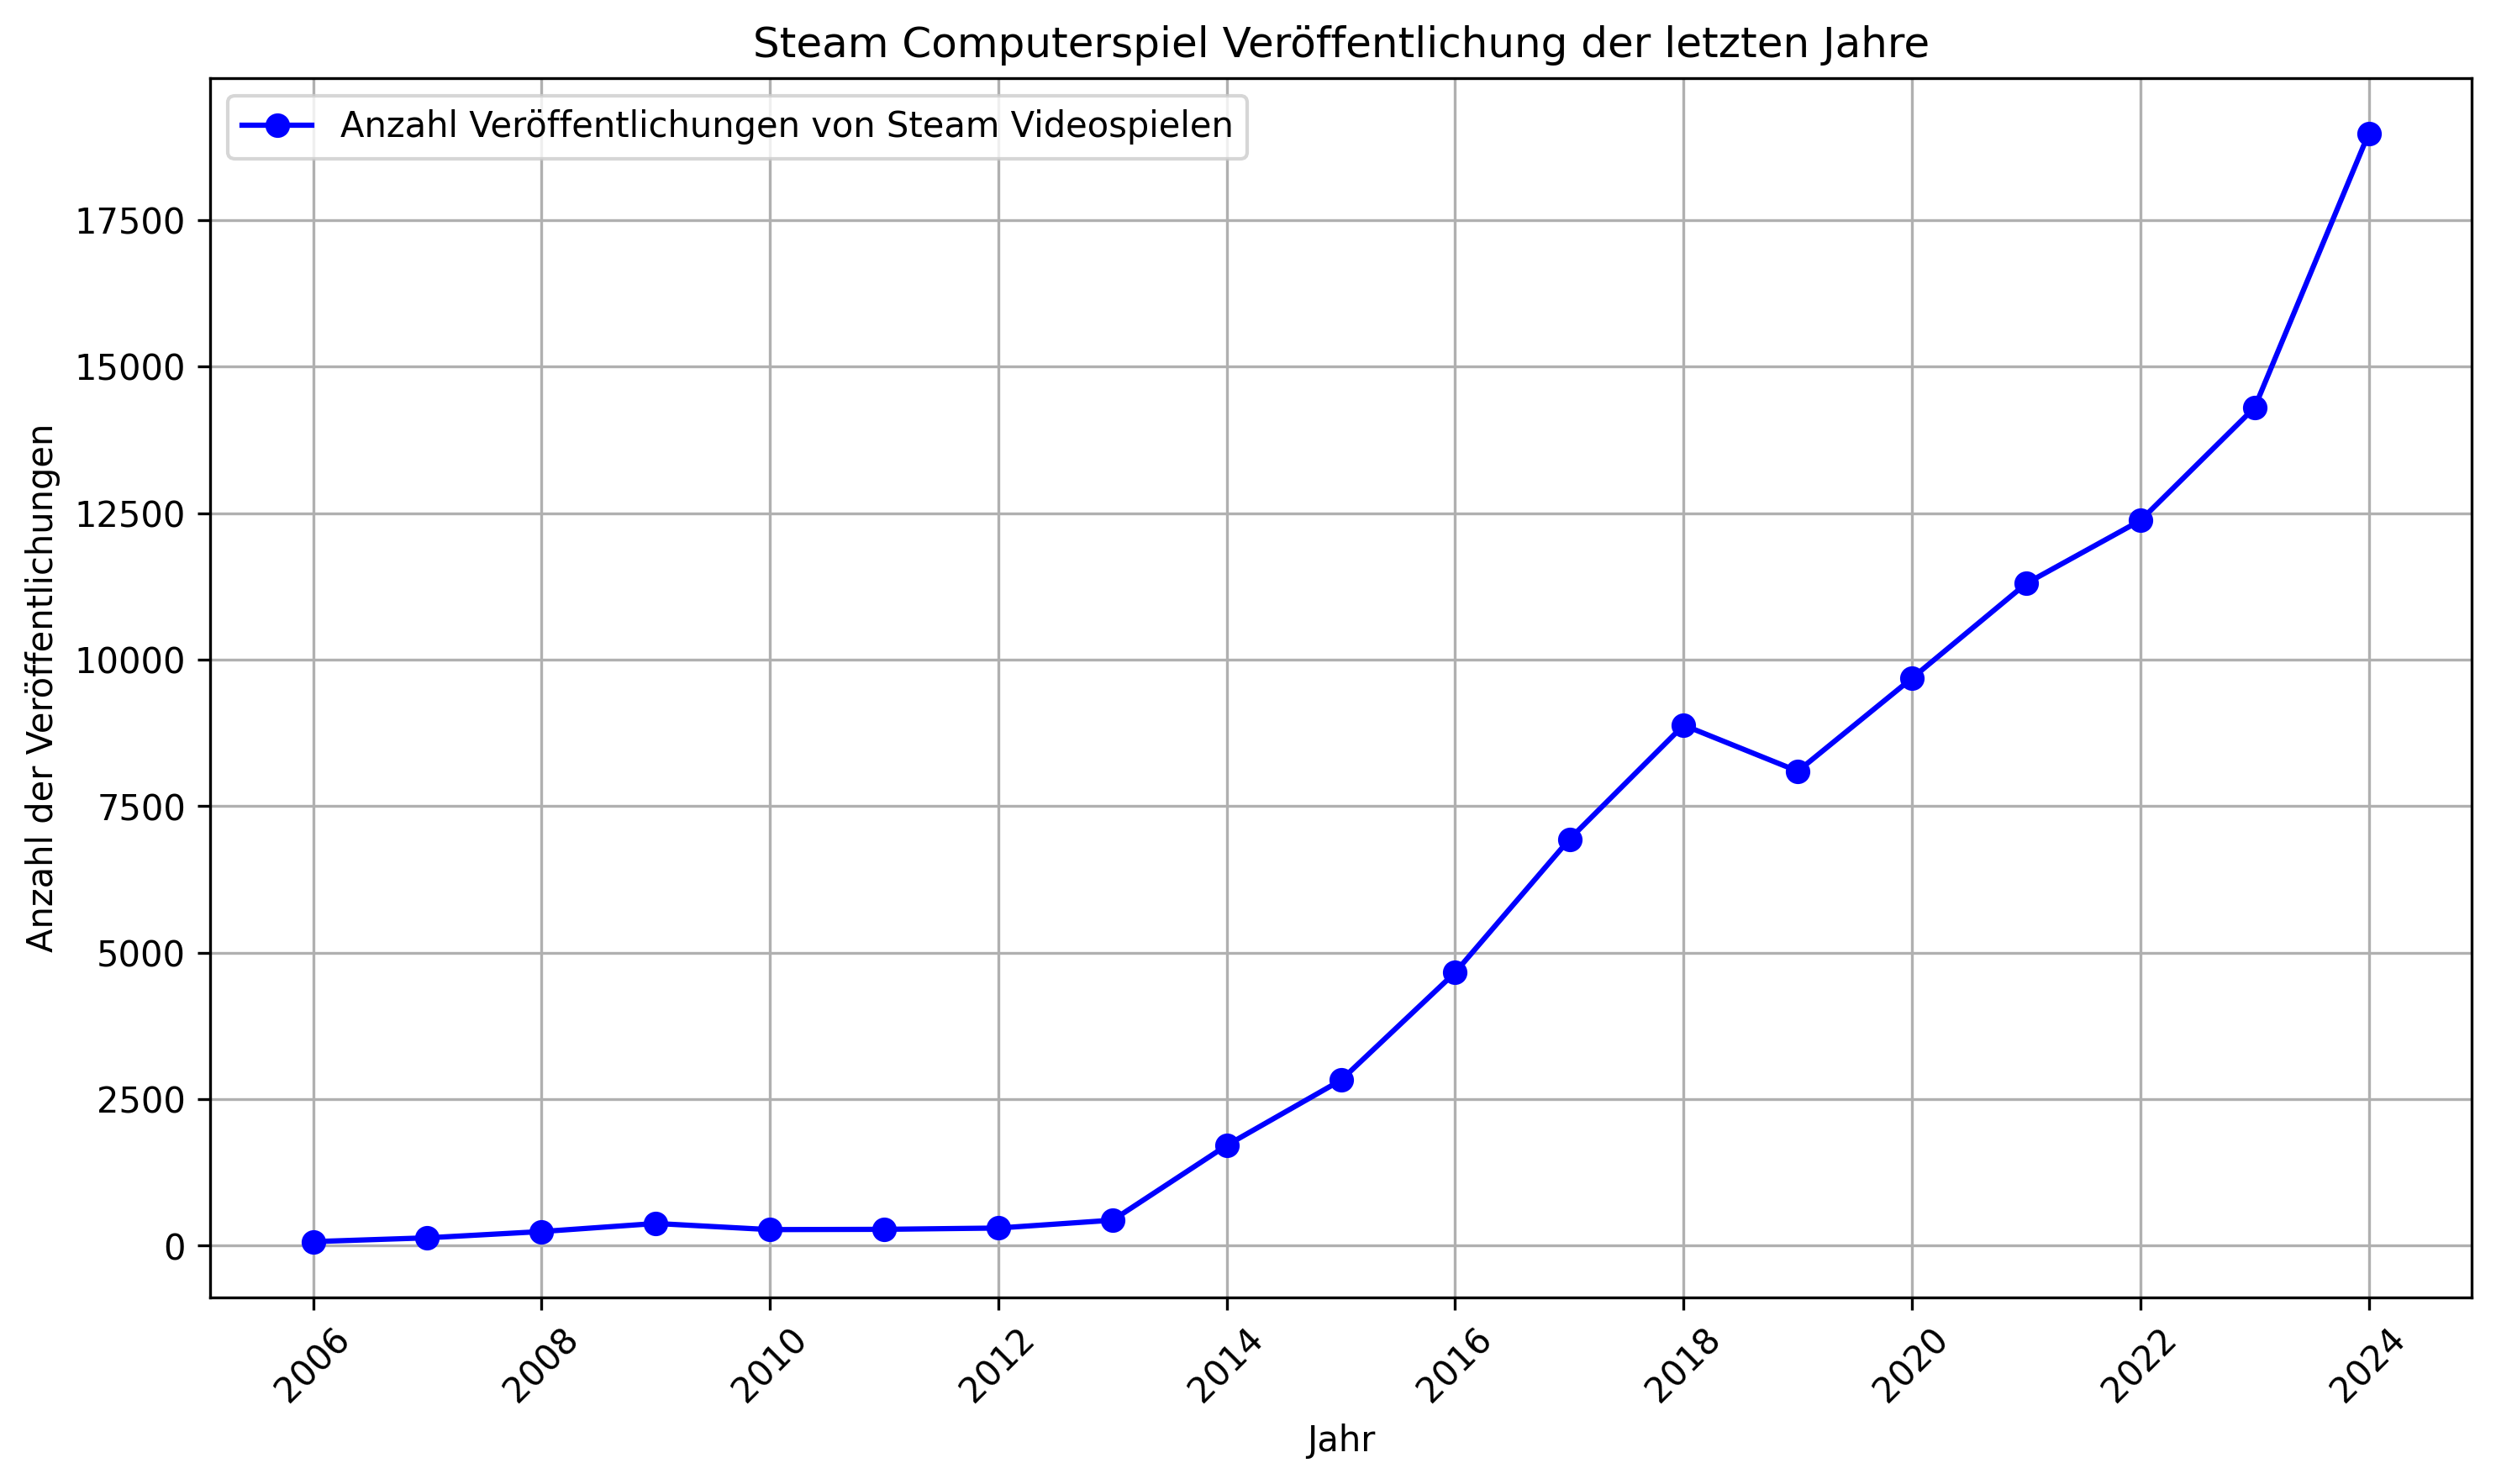
\includegraphics[width=15cm]{state_of_the_art/steam_veroffentlichungen}
	\captionsetup{justification=justified, format=plain}
  \caption{Computerspiel Ver�ffentlichungen auf Steam �ber die Jahre}
  \label{SteamDB Statistik}
\end{figure}

Folglich kann davon ausgegangen werden, dass es Stakeholder gibt, die sich f�r Videospiele interessieren.



\section{Game-Engines}

Seit der Doom-Engine sind neue \hyperref[chap:game engines]{Game-Engines} entstanden und haben sich weiterentwickelt. Zu den g�ngigen zug�nglichen Game-Engines geh�ren: Unreal-Engine, Unity und Godot. Godot ist dabei die j�ngste Game-Engine und konkurriert mit der Unity. In den letzten Jahren hat Unity das Vertrauen von Entwicklerstudios verloren. Viele Entwicklerstudios wechseln nun in den letzten Jahren ihre Game-Engine. Das folgende Teilkapitel wird den derzeitgen Stand von den drei Game-Engines beschreiben.  

%Gro�e Entwicklerstudios besitzen ihre eigene Game-Engine. So nutzt beispielsweise das deutsche Entwicklerstudio Crytek die Cryengine. Eine eigene Game-Engine zu entwickeln ben�tigt zus�tzliche Ressourcen. Dagegen ist dies bei Indie-Entwicklerstudios schwer umsetzbar. Denn sie haben weniger Arbeitskr�fte als gro�e Entwicklerstudios und entwickeln Videospiele ohne finanzielle Unterst�tzung gr��erer Unternehmen. Dadurch sind Indiestudios von m�glichst kosteng�nstigen Game-Engines abh�ngig.\autocite{holfeld2024relevancegodotengineindie}

\subsection{Unity}

Unitys Versuch, ein neues Geb�hrenmodell f�r Entwickler einzuf�hren, hat die Wahrnehmung der \hyperref[chap:game engines]{Game-Engine} als entwickler-freundliches Programm negativ beeinflusst. So k�ndigte Unity September 2023 eine �nderung des Geb�hrenmodells, zum Anfang des Jahres 2024, an. Die neue Regelung sah vor, dass Entwickler ab einem Umsatz von 200.000 US-Dollar und mindestens 200.000 Installationen f�r jede Erstinstallation eines Spiels 20 US-Cent an Unity zahlen sollen.\autocite{golem1}

Die �nderung h�tte finanzielle Folgen f�r viele Entwicklerstudios, insbesondere f�r Indieentwickler. Videospielentwickler sprachen davon, dass Unity sie in den Bankrott treiben w�rden. So berichtete eine Indiestudio f�r Mobile-Games, dass diese rund 108 Prozent ihrer Bruttoeinnahmen abf�hren m�ssten. Das Entwicklerstudio Mega Crit k�ndigte sogar an eines ihrer erfolgreichen Videospiele zu entfernen. Andere Videospielentwickler k�ndigten an zur Konkurrenz von Unity zu wechseln. So hat das Entwicklerstudio Mega Crit angek�ndigt, ihr Projekt auf eine andere Game-Engine umzustellen, obwohl sie bereits seit Jahren mit Unity arbeiteten.\autocite{golem1} 

Aufgrund der Kritik von Entwicklerstudios hat sich Unity nach der Ank�ndigung des Geb�hrenmodells entschuldigt. Darauf folgend k�ndigte Unity an, die Richtlinien zu �ndern unter Absprachen mit Stakeholdern.\autocite{golem2} Au�erdem k�ndigte der ehemalige CEO von Unity John Riccitiello seinen R�cktritt an.\autocite{golem5} Matt Bromberg hat infolgedessen seine Position eingenommen und September 2024 angek�ndigt auf das alte Geb�hrenmodell zur�ckzukehren.\autocite{unity1}

Trotz der Ank�ndigung das Geb�hrenmodell zu �ndern, sprachen viele Entwicklern von einem Vertrauensverlust. So hat Entwicklerstudio Re-Logic, welches Godot mit Spenden unterst�tzt hat, weiterhin Kritik an Unity ge�u�ert und ihre Vorgehen infrage gestellt.\autocite{golem3}

\subsection{Godot}

Godot ist die \hyperref[chap:game engines]{Game-Engine} auf der die Implementierung umgesetzt wurde. Godots Relevanz ist in den letzten Jahren gestiegen. Die Game-Engine wird �fter mit der Unity-Engine verglichen, welche ebenfalls von Indie-Entwicklerstudios benutzt wird. Als Game-Engine konzentriert sich Godot auf die 2D-Umgebung, aber auch die 3D-Umgebung wird gef�rdert. Sie ist jedoch nicht so weit entwickelt wie die 3D-Umgebung der Unreal-Engine.

Aufgrund der �nderungen im Geb�hrenmodell von Unity haben sich viele Videospielentwickler, die zuvor auf Unity als Entwicklungsplattform setzten, nach Alternativen bei der Konkurrenz umgesehen. Im Vergleich zu Unity bietet Godot eine gr��ere Sicherheit vor Lizenz�nderungen sowie Mehrkosten, da es sich bei Godot um ein Open-Source Programm handelt. Lizensiert ist Godot unter der MIT-Lizenz, wodurch Godot im Gegensatz zu Unity zu jedem Zweck genutzt, bearbeitet und weitervertrieben werden kann.\autocite{golem4} Aufgrund der genannten Punkte ist Godot eine zunehmend bevorzugte Wahl f�r Entwickler und eine Konkurrenz zu Unity. Unter den Godot Dokumentationen gibt es explizite Anleitungen, wie man von Unity auf Godot migrieren kann.\footnote{https://docs.godotengine.org/en/3.1/getting_started/editor/unity_to_godot.html}

\subsubsection{Investitionen}

Godot ist im Laufe seiner Entwickler, neben Videospielentwickler, auch f�r gr��ere Unternehmen interessant geworden. So hat \textit{Microsoft} 2017 eine \$24.000 Spende an Godot get�tigt, da C# mit Godot kompatibel wurde. Der Spieleentwickler \textit{Epic Games} hat 2020 eine \$250.000 Spende get�tigt, da Epic Games OpenSource Projekte f�rdert, welche 3D-Grafik Umgebungen weiterentwickeln.\autocite{megagrant} Man beachte, dass Epic Games selbst die Unreal Engine entwickelt und eigentlich ein Konkurrent ist. Im Jahr 2020 und 2021 hat \textit{Meta} an Godot gespendet, damit diese die XR Umgebung f�r Godot entwickeln. Auch \textit{Khronos Group} m�chte die XR Umgebung weiterentwickeln und unterst�tzt Godot aufgrund der Integration von \textit{OpenXR} \autocite{khronos}. Entwicklerstudios selbst spenden ebenfalls an Godot. So hat das Entwicklerstudio \textit{Re-Logic} eine \$100.000 Spende im Jahr 2023 get�tigt.\autocite{gdfd2023} 

Godot wird haupts�chlich �ber den Godot Development Fund finanziert. Weitere Investoren kann man auf der Webseite von Godot einsehen.\footnote{https://godotengine.org/} Folglich kann ein Trend an Investoren f�r Godot erkannt werden und somit auch die Relevanz von Godot als \hyperref[chap:game engines]{Game-Engine}.


%https://www.golem.de/news/spieleindustrie-unity-oder-godot-wer-gewinnt-das-engine-duell-2310-178099.html (4. Oktober 2023)
%%Unitys undurchsichtige Preispolitik hat Kunden nachhaltig verschreckt. Ein Open-Source-Projekt schickt sich nun an, der Profi-Engine Konkurrenz zu machen.
%Unity, die Firma hinter der laut Sch�tzungen von SteamDB mit knapp 40.000 Titeln meistgenutzten Engine im wichtigsten Shop f�r PC-Games
%%Derzeit besonders im Kommen: Godot, ein Open-Source-Projekt mit flexibler Scripting-Unterst�tzung und �hnlichem Baukastenprinzip wie Unity, in der Vergangenheit vor allem spezialisiert auf schlanke 2D-Projekte.
%Durch die zus�tzliche Ansprache des .Net-Frameworks kann das bei leistungshungrigen Anwendungen in manchen F�llen zu Performance-Einbu�en f�hren. Daf�r ist C# beispielsweise aufgrund automatisierter Speicherverwaltung einsteigerfreundlicher, Stichwort garbage collector.
%Speicherlecks werden dadurch vermieden. �brigens: Per Reference Counting ist die Speicheroptimierung auch in Godots hauseigener Skriptsprache gegeben.
%%Der gro�e Vorteil von Godot: Anders als bei Unity kommt hier die Frage nach Geb�hren und Umsatzbeteiligungen gar nicht erst auf. Godot ist ein klassisches Open-Source-Projekt und wird von der Community erweitert, die Projektleitung liegt bei den Entwicklern und Gr�ndern Juan Linietsky und Ariel Manzur.
%Lizensiert ist Godot unter der MIT-Lizenz, hei�t: Anders als beim propriet�ren Unity kann die Engine zu jedem Zweck genutzt, bearbeitet und weitervertrieben werden. Die Finanzierung des Projects findet also nicht �ber monatliche und erfolgsabh�ngige Geb�hren statt, sondern haupts�chlich �ber den Godot Development Fund, in den knapp 1.500 Mitglieder derzeit zusammen etwa 50.000 Euro pro Monat einzahlen.


\subsection{Unreal-Engine}

Die Unreal-Engine ist ein \hyperref[chap:game engines]{Game-Engine} die sich auf 3D Umgebung spezialisiert hat. Sie ist besonders f�r gr��ere Entwicklerstudios geeignet, da sie in ihren Funktionen und Eigenschaften komplexer ist. 

Gro�e Entwicklerstudios besitzen eigene Game-Engines auf denen sie ihre Videospiele entwickeln. Eine eigene Game-Engine hat seine Vor und Nachteile. Einerseits hat das Entwicklerstudio die M�glichkeit ihre Werkzeuge selbst�ndig zu erstellen, �ndern und erweitern sowie Kosten f�r Lizenzen zu sparen, andererseits muss man das Personal ausbilden, wenn die Game-Engine au�erhalb nicht zug�nglich ist. So nehmen Entwicklerstudios die Lizenzkosten einer Game-Engine in Kauf und wechseln beispielsweise auf eine �ffentlich zug�ngliche Game-Engine, wie Unreal-Engine. So wechselt das Entwicklerstudio, der Halo Reihe, auf die Unreal-Engine, um einfacher, neue Mitarbeiter zu finden, die gleich in die Produktion einsteigen k�nnen.\autocite{golem6} Das Entwicklerstudio CD Project Red wechselte ebenfalls von ihrer Red-Enigne auf die Unreal-Engine. Der Grund wiederum war, die technische Ausrichtung eine Videospieles fr�hzeitig festlegen zu k�nnen, da in der Vergangenheit viel Aufwand in die kontinuierliche Anpassung und Weiterentwicklung der Red-Engine investiert wurde.\autocite{golem7} Daraus l�sst sich der Trend erkennen, dass sich die Unreal-Engine als standard Framework der Game-Engines etablieren kann.

\section{Entscheidungssysteme in der Game AI}

In der Funktionalit�t von \hyperref[chap:entscheidungssysteme]{Entscheidungssystemen} wie Behavior Trees (BT), Finite State Machines (FSM) und Goal-Oriented Action Planning (GOAP) wurde bereits eingehend auf deren Grundlagen eingegangen. Das folgende Kapitel widmet sich nun der praktischen Anwendung dieser drei Systeme sowie fortschrittlicher Methoden des maschinellen Lernens in der modernen Videospielentwicklung und Forschung.

Es muss angemerkt werden, dass es nicht das eine beste Entscheidungssystem gibt. Im Grundlagenkapitel Game-AI wurde bereits erl�utert, dass es abseits der Entscheidungssysteme weitere Komponenten gibt, welche die Immersion des NPC beeinflussen. Faktoren wie die Aktionen, die ein NPC ausf�hrt, die Wahrnehmung der Spielwelt durch den NPC oder die Navigation zu einer bestimmten Koordinate tragen zur Immersion bei. Ein Entscheidungssystem soll dabei logische Aktionen des NPC in seinem derzeitigen Zustand w�hlen. Je nachvollziehbarer diese Aktionen sind, desto st�rker ist die Immersion.

Videospielentwickler verwenden f�r ihre NPCs oft nicht nur ein einzelnes Entscheidungssystem. So nutzten die Videospielentwickler des Action-Rollenspiel \textit{Final Fantasy XV (2016)} ein Entscheidungssystem, das sowohl BTs als auch FSMs integriert \textit{(AI Graph Editor)}. Dies zeigt, dass die Kombination mehrerer Entscheidungssysteme eine sinnvolle Alternative darstellen kann.

So werden in Foren bis heute diskutiert, welche Videospiele mit ihrer Game-AI hervorstechen. Besonders werden Videospiele gelobt, welche GOAP als Entscheidungssystem umgesetzt haben. Zu diesen Spielen geh�ren unter anderem \textit{F.E.A.R. (2005)} und \textit{S.T.A.L.K.E.R. (2007)}.
In Online Artikeln wie \autocite{vanceai}, \autocite{techopedia} und \autocite{gamerant} werden beide Titel weiterhin als Beispiele f�r herausragende Game-AI genannt. Sie stehen trotz ihren Alters dabei in einer Reihe mit aktuelleren Spielen, wie \textit{Alien Isolation (2014)} oder \textit{The Last of Us (2013)}.
Angemerkt sein noch, dass es schwierig zu sagen ist, welche Entscheidungssysteme aktuell in Videospielen eingesetzt werden. Videospieleentwickler geben selten detaillierte Informationen �ber die von ihnen verwendeten Entscheidungssysteme. Die Tabelle X soll dabei einige bekanntere Videospiele und ihre Entscheidungssysteme darstellen.


\subsection{Fortschrittliche Methoden des maschinellen Lernens}

Der Trend von fortschrittliche Methoden des maschinellen Lernens, hat an Bedeutung gewonnen. Die Methoden spielen zwar eine immer gr��ere Rolle im allt�glichen Leben, haben jedoch einen eher geringeren Einfluss im Bereich der Game AI. Diese Methoden erfordern gro�e Mengen an Daten f�r das Training und es ist �u�erst schwierig, sie auf unvorhergesehene Situationen, wie in Videospielen, zu testen. \autocite{U2023}

Es existieren wenige ver�ffentlichten Studien, die ihre Anwendung als \hyperref[chap:entscheidungssysteme]{Entscheidungssystem} f�r NPC dokumentieren, \autocite{U2023} daher werden diese nicht weit erl�utert. Dennoch gibt es Videospiele, welche diese Methoden f�r bestimmte Funktionen von NPC verwendet werden und in den folgenden Abschnitten erl�utert werden. Es w�re interessant diese Methoden ausf�hrlicher in der akademischen Forschung Richtung Game AI zu sehen, insbesondere in Richtung Entscheidungssysteme.

Die Methoden des maschinellen Lernens kann man in supervised learning (SL), unsupervised learning (UL) und reinforcment learning(RL) unterteilen. So bekommt SL gelabelte Daten und UL Rohdaten mit denen sie trainieren. W�hrend RL auf Basis der Umgebung lernt und durch richtige Aktionen belohnt wird. So wird Deep Learning, ein Teil von SL, f�r Spracherkennung und natural language processing benutzt. Im Strategiespiel StarCraft wird RL f�r das \textit{micromanagement} der NPC benutzt. \autocite{inbook}

Die Evolution�re-Algorithmen sind inspiriert durch Darwins Theorie der Evolution. Sie optimieren dabei eine Population, wo jedes Individuum eine L�sung repr�sentiert und mit einer Fitness-Wert gekennzeichnet ist. Durch Iterationen finden Selektionen und Mutationen in der Population statt, welche den Fitness-Wert der optimalen L�sung erh�hen. Im Bereich der Videospielentwicklung optimierte der Algorithmus beispielsweise die Baureihenfolge der NPC im Strategiespiel StarCraft. \autocite{inbook}


\subsection{Finite State Machines}

In den fr�hen Tagen der Spielentwicklung waren FSM ausreichend, um eine Entscheidungsfindung f�r NPC bereitzustellen. So wurde bereits im Grundlagenkapitel das Videospiel \textit{Half-Life (1998)} erw�hnt. Auch abseits des FPS-Genre wurde die FSM verwendet. 2D-Videospiele wie Pac-Man und Sonic nutzten FSM, um das Verhalten ihrer NPC zu definieren. \autocite{U2023}

Die Umsetzung einer FSM wird oft als Einstieg in die \hyperref[chap:entscheidungssysteme]{Entscheidungssysteme} der Game-AI empfohlen. Sie sind die am h�ufigsten verwendete Methode zur Entscheidungsfindung, bei NPC mit geringer Komplexit�t. Bis heute machen sie den Gro�teil der in Spielen eingesetzten Entscheidungssysteme aus \autocite{AIgames}.

Bei komplexen Videospielen wird �fter eine Hierarchical State Machine (HFSM) umgesetzt. Es handelt sich dabei um eine Erweiterung der FSM. Eine HFSM bietet im Gegensatz zur FSM die M�glichkeit, Zust�nde zu verschachteln und Hierarchien zwischen Zust�nden zu definieren. Dies bietet den Vorteil eine bessere �bersicht �ber die Zust�nde zu haben, vor allem bei komplexen NPC. \autocite{AIgames}


\subsection{Behavior Trees}
\label{chap:sota bt}

BT sind in den Vordergrund der Game-AI ger�ckt. So bieten sie einen intuitiveren Ansatz als fr�here Techniken wie FSM, die oft komplexe Datenstrukturen erforderten die bei einer Vergr��erung einen schlecht strukturierten Code erzeugen \autocite{qlbt}. Im Kapitel wurden bereits die Videospiele \textit{Alien Isolation (2014)} und \textit{The Last of Us (2013)} als erfolgreiche Titel in Richtung Game-AI beschrieben. Beide Titel setzen den BT als \hyperref[chap:entscheidungssysteme]{Entscheidungssystem} um. Der BT wurde mit dem Videospiel Titel \textit{Halo 2 (2004)} eingef�hrt.

Schaut man sich Studien bez�glich Entscheidungssysteme an, so kann man den Behavior Tree als Trend erkennen. So besitzt das BT-System aktuellere Studien, auch au�erhalb der Videospielentwicklung wie \autocite{btuav} und \autocite{8963263}. Studien, wie \autocite{rbt} und \autocite{qlbt}, besch�ftigen sich mit dem Einsatz des maschinellen Lernens, um einen Behavior Tree zu optimalisieren. So kann das {QL-BT} System \autocite{qlbt} mittels RL ein BT optimalisiert werden, indem es die Knoten eines Baumes reorganisiert. Das System soll unter anderem ein BT simplifizieren und Code Duplikationen reduzieren.


\subsection{GOAP}

Im Vergleich zu Behavior Trees ist der Forschungsstand zu GOAP im Bereich der Game-AI weniger umfangreich. Dennoch existieren Studien, die Ans�tze zur Nutzung von GOAP beschreiben. So wurde in \autocite{Schwab2021} eine Methode beschrieben, die mittels GOAP ein Behavior Tree konstruiert. Da das manuelle Erstellen von BTs eine aufwendige und stark parameterabh�ngige Aufgabe darstellt, bietet die automatische Konstruktion eine Alternative. Diese Methode beobachtet zun�chst das Verhalten, das GOAP in einer Monte-Carlo-Simulation zeigt, und nutzt anschlie�end einen genetischen Algorithmus, um einen geeigneten Behavior Tree zu entwickeln. Die resultierenden Behavior Trees zeichnen sich dadurch aus, dass sie verst�ndlich, anpassbar und ebenso leistungsf�hig wie manuell erstellte Modelle sind. \autocite{Schwab2021}

Im Bereich der Videospielentwicklung ist das GOAP System in den Hintergrund ger�ckt. Derzeit gibt es einen Mangel an Bibliotheken, die Videospielentwicklern zur Verf�gung stehen und GOAP Systeme beinhalten. Studien wie \autocite{sielicki2018adaptation} fordern mehr Bibliotheken in Richtung \textit{Goal oriented action planning} Systeme. So hat die Studie selbst das GOAP System in der \hyperref[chap:game engines]{Game-Engine} Unreal Engine umgesetzt.


\begin{sidewaystable}[h]
  \label{Videospiele und ihre Entscheidungssysteme}
  \renewcommand{\arraystretch}{1.2}
  \centering
  \small
    \begin{tabularx}{0.95\textwidth}{l l x x x x}
			\toprule
      \textbf{Videospiel} & \textbf{Entscheidungssystem} & \textbf{Genre} & \textbf{Entwicklerstudio} & \textbf{Erscheinungsjahr} & \textbf{Quelle} \\
			\toprule
			Driver: San Francisco & BT & Rennspiel & Ubisoft & 2011 & \autocite{Ocio2021} \\
      Spore & BT & Strategie & Maxis & 2008 & \autocite{spore} \\
      Halo 2 & BT & FPS & Bungie & 2004 & \autocite{aiag} \\
      Tomb Raider & GOAP & Action & Eidos Montreal & 2013 & \autocite{goap_gdc} \\
      Half-Life & FSM & FPS & Valve & 1998 & \autocite{halflife} \\
      S.T.A.L.K.E.R.: Shadow of Chernobyl & GOAP & FPS & GSC Game World & 2007 & \autocite{sielicki2018adaptation} \\
      No One Lives Forever 2 & FSM & FPS & Monolith Productions & 2002 & \autocite{fear} \\
      F.E.A.R & GOAP & FPS & Monolith Productions & 2005 & \autocite{fear} \\
      Deus Ex: Human Revolution & GOAP & FPS & Eidos Montreal & 2011 & \autocite{sielicki2018adaptation} \\
      Middle-earth: Shadow of Mordor & GOAP & Rollenspiel & Monolith Productions & 2014 & \autocite{goap_gdc} \\
      Alien: Isolation & BT & FPS & Creative Assembly & 2014 & \autocite{vsvelch2020should} \\
      The Last of Us & BT & TPS & Naughty Dog & 2013 & \autocite{panwar2022npcaiuscase} \\
      Mafia III & BT & TPS & 2K Games & 2016 & \autocite{holba2021open} \\
      \bottomrule
    \end{tabularx}
		\caption{Videospiele der letzten Jahre und ihre Entscheidungssysteme}
\end{sidewaystable}

\input{kapitel/Lösungskonzept}
\input{kapitel/Implementierung Lösungskonzept}
\chapter{Ergebnis}
\label{chap:ergebnis}

In diesem Kapitel werden die Entscheidungssysteme FSM, BT und GOAP aus der Erfahrung durch die Implementierung \autocite{oleg}, Benchmarks, wissenschaftlicher Literatur verglichen und folglich bewertet.

Der Vergleich wird sich auf die folgenden Punkte fokussieren: Erlernbarkeit, Umsetzung, Skalierbarkeit, Debugging, Performance und Speicherverbrauch. 

F\"{u}r den Vergleich der Performance und Speicherverbrauch werden Ergebnisse von Benchmarks einbezogen.

\section{Ergebnisse der Implementierung}

In Kapitel \ref{chap:loesungskonzept} wird das L\"{o}sungskonzept beschrieben. Dort wird erl\"{a}utert, dass die Bewertung der Entscheidungssysteme auf wissenschaftlicher Literatur sowie praktischen Erfahrungen basiert. Letztere ergeben sich aus der Implementierung der drei Entscheidungssysteme in einem spezifischen Szenario und flie\ss{}en in die abschlie\ss{}enden Vergleich ein. Die Implementation des Szenario wird im Kapitel \ref{chap:implementierung lk} beschrieben.


\subsection{Erlernbarkeit}
\label{chap:erlernbarkeit}

Die Erlernbarkeit beschreibt, wie komplex es f\"{u}r Entwickler ist, das jeweilige Entscheidungssystem zu verstehen und anzuwenden. Sie h\"{a}ngt von mehreren Faktoren ab. Dazu geh\"{o}rt die Verst\"{a}ndlichkeit der Konzepte, die Verf\"{u}gbarkeit von Dokumentationen sowie die notwendigen Vorkenntnisse f\"{u}r die Nutzung.

%FSM
Die FSM ist leicht verst\"{a}ndlich. Sie wird h\"{a}ufig als Einf\"{u}hrungsbeispiel in die Game-AI Entscheidungssysteme genommen, wie es in vielen Fachb\"{u}chern, wie \autocite{AIgames, aiag}, zur Game-AI ersichtlich ist. Es gibt gen\"{u}gend Internet Quellen, die eine FSM Implementation dokumentieren. Haupts\"{a}chlich werden Kenntnisse \"{u}ber endliche Automaten ben\"{o}tigt. Im Vergleich zu den anderen Entscheidungssystemen ist sie am einfachsten zu erlernen.

%BT
Aufgrund der verschiedenen Task-Kategorien ist der BT anspruchsvoller in der Anwendung und Einf\"{u}hrung als die FSM. Kenntnisse in der Graphentheorie, insbesondere \"{u}ber gerichtete Graphen\ref{}, sind f\"{u}r das Verst\"{a}ndnis eines BT von Vorteil. Sie hat ebenfalls viele Dokumentationen zur Implementation.

%GOAP
Mit dem dynamischen System kommt die Komplexit\"{a}t der Funktionsweise. GOAP wird im Gegensatz zu den anderen beiden Entscheidungssysteme f\"{u}r fortgeschrittene Entwickler empfohlen. Kenntnisse im Bereich von Graphentheorie und Suchalgorithmen k\"{o}nnen das Verst\"{a}ndnis und die Nutzung von GOAP jedoch erheblich erleichtern. In Bezug auf Dokumentation und verf\"{u}gbare Bibliotheken weist GOAP deutliche M\"{a}ngel auf. Wie bereits im Kapitel \ref{chap:goap sota} erl\"{a}utert, fordern Studien wie \autocite{sielicki2018adaptation} eine st\"{a}rkere Verbreitung von Dokumentationen und Bibliotheken f\"{u}r GOAP. Im Vergleich zu den anderen Entscheidungssystemen gibt es zu GOAP deutlich weniger Dokumentation.


\subsection{Umsetzung}
\label{chap:umsetzung}

Bei der Umsetzung liegt der Fokus auf der praktischen Umsetzung des Entscheidungssystems in der Game-Engine Godot. Dabei wird betrachtet, wie aufwendig die Implementierung der Funktionsweise und Architektur des Entscheidungssystems ist sowie das designen der NPCs.

%FSM
Die FSM ist als Ad-Hoc-Authoring Methode ein statisches Entscheidungssystem und in Godot unkompliziert zu implementieren. Die Architektur besteht dabei aus einer Knoten Klasse und einer Koordinaten Klasse. Einen Knoten zu erstellen und diesen mit Aktions Komponenten zu erg\"{a}nzen ist einfach. Doch mit der gr\"{o}\ss{}e der Komplexit\"{a}t eines NPC steigt der Aufwand die FSM instandzuhalten, da mit der Anzahl an Aktionen die Anzahl der Knoten im Graphen steigen.

%BT
Auch der BT ist als Ad-Hoc-Authoring Methode ein statisches Entscheidungssystem und in Godot unkompliziert zu implementieren. Im Vergleich zur FSM hat er aber durch die verschiedenen Task-Typen eine komplexere Architektur. Die Architektur ist aber unaufwendig zu realisieren und man hat durch die verschiedenen Kategorien der Tasks die M\"{o}glichkeit komplexere NPC Verhalten umzusetzen. Dennoch wird der BT als zu statisch empfunden.\autocite{aiag}. Zudem m\"{u}ssen Entwickler viel Zeit darauf verwenden, passende BT-Knoten zu erstellen und sie mit den richtigen Verhaltensweisen verkn\"{u}pfen.\autocite{Schwab2021} Wie bereits in den zuvor erl\"{a}uterten Studien aus dem Kapitel\ref{chap:bt sota}, kann die Struktur eines BT jedoch durch Methoden wie maschinelles Lernen oder GOAP automatisch generiert werden.

%GOAP
Der GOAP ist als dynamisches System das komplexeste der drei Entscheidungssysteme, wenn es um die Implementierung geht. Sie erfordert ein tiefgehendes Verst\"{a}ndnis der Funktionsweise von GOAP. Hat man diese jedoch verstanden, k\"{o}nnen immersive NPC-Verhalten designed werden. Hinzu kommt das Godot 4.3 Datenstrukturen, wie Sets und PriorityQueues nicht beinhaltet, sodass diese f\"{u}r bessere Zugriffszeiten selbst implementiert werden m\"{u}ssen. Beim Designen von NPC-Verhalten ist insbesondere die Zuweisung der Kosten einer Aktion eine Herausforderung \autocite{Schwab2021}. Doch mit der Komplexit\"{a}t ist es m\"{o}glich immersive NPC-Verhaltensweisen zu programmieren.


\subsection{Skalierbarkeit}
\label{chap:skalierbarkeit}

Der Punkt Skalierbarkeit bewertet, wie komplex es ist das System mit Aktionen zu erweitern oder bestehende zu \"{a}ndern.

%FSM
Die FSM ist schwer skalierbar. Wird eine Aktion (Knoten) ge\"{a}ndert oder hinzugef\"{u}gt, so muss der Graph der FSM angepasst werden. Eine \"{A}nderung oder das Hinzuf\"{u}gen einer Aktion kann dazu f\"{u}hren, dass andere Knoten die mit der Aktion in Verbindung stehen ebenfalls ge\"{a}ndert werden m\"{u}ssen. Dies kann zu einem Dominoeffekt f\"{u}hren, bei der eine Kette an Knoten ge\"{a}ndert werden muss und wiederum Zeitaufwand bedeutet. Zust\"{a}nde und \"{U}berg\"{a}nge sollten dabei vollst\"{a}ndig definiert sein, so dass der NPC nicht in falschen Zust\"{a}nden h\"{a}ngen bleibt. Die FSM wird mit jeder Erweiterung an Aktionen auch un\"{u}bersichtlicher. So hatte das Spiel Half-Life (1998) ca. 80 so genannte Tasks, die alle einem Zustand zugewiesen sind. Die Un\"{u}bersichtlichkeit f\"{u}hrt zur erh\"{o}hten Komplexit\"{a}t des Entscheidungssystems. Au\ss{}erdem k\"{o}nnen Leistungsprobleme auftreten, insbesondere bei einer \"{u}berm\"{a}\ss{}igen Anzahl von Knoten. \autocite{U2023}

%BT
Wie auch die FSM ist der BT ein statisches Entscheidungssystem. Er ist jedoch im Vergleich zu FSM skalierbarer. Die Aktionen eines BT sind durch die Tasks loser gekoppelt und m\"{u}ssen sich nicht gegenseitig stark beeinflussen. So kann bei einer Erweiterung ein neuer Zweig hinzugef\"{u}gt werden mit seinen eigenen Tasks, ohne viele bestehende Aktionen oder Strukturen zu ver\"{a}ndern.\autocite{aiag} Allerdings kann auch ein BT mit zunehmender Anzahl an Aktionen un\"{u}bersichtlich werden. Erfahrung zeigt, dass das Lesen und Verstehen eines BT schwieriger ist als bei einer FSM.

%GOAP
Das Entscheidungssystem GOAP ist hinsichtlich der Skalierbarkeit den zuvor beschriebenen Systemen \"{u}berlegen. Es m\"{u}ssen bei neuen Aktionen oder \"{A}nderungen bestehender Aktionen keine manuellen Verkn\"{u}pfungen get\"{a}tigt werden, da alle Aktionen unabh\"{a}ngig voneinander existieren. Die Reihenfolge der Aktionsausf\"{u}hrung wird dynamisch durch GOAP bestimmt, was es zu einem anpassungsf\"{a}higen Entscheidungssystem macht.


\subsection{Debugging}
\label{chap:debugging}

Das Debugging beschreibt, wie komplex Fehler im Entscheidungssystem gefunden und behoben werden k\"{o}nnen. 

%FSM
Das Debuggen einer FSM ist vergleichsweise einfach \autocite{review_game_ai}, da ihre Struktur statisch ist und sich nicht dynamisch ver\"{a}ndert. Durch die Visualisierung des Graphen l\"{a}sst sich nachvollziehen, welche Knoten zur ausgef\"{u}hrten Aktion gef\"{u}hrt haben. Speichert man zus\"{a}tzlich die zuletzt durchlaufenen Knoten und gibt diese aus, kann der Ablauf noch besser nachvollzogen und m\"{o}gliche Fehlerquellen leichter identifiziert werden.

%BT
Auch das Debuggen soll laut Quellen wie \autocite{aiag, review_game_ai} einfacher sein. Insbesondere durch die Tasks und ihre R\"{u}ckgabewerte l\"{a}sst sich nachvollziehen, welche Pfade im Baum durchlaufen wurden. Eine Visualisierung ist ebenfalls m\"{o}glich und kann das Verst\"{a}ndnis zus\"{a}tzlich erleichtern.

%GOAP
Ein Nachteil der mit dem dynamischen System kommt ist das Debuggen. Es ist es schwierig, die m\"{o}gliche Reihenfolge der Aktionen vorherzusagen, da GOAP die Aktionen basierend auf ihren Kosten und Zust\"{a}nden ausw\"{a}hlt und nicht durch statische Verbindungen, wie es in Ad-hoc-Behavior-Authoring-System der Fall ist. Eine m\"{o}gliche L\"{o}sung w\"{a}re eine Visualisierung des Suchbaums, wie er durch den A*-Algorithmus in GOAP generiert wird. Eine solche Darstellung w\"{u}rde aufzeigen, welche Aktionen potenziell in Frage kamen und welche letztendlich priorisiert wurden. Allerdings ist die Implementierung dieser Visualisierung deutlich komplexer als bei einer FSM oder einem BT.


\section{Ergebnisse der Benchmarks}
\label{chap:erbnisse benchmark}

Die Abbildung \ref{fig:bps benchmark} zeigt die Ergebnisse des Performance-Benchmarks. Laut Quellen wie \autocite{aiag} gilt insbesondere GOAP als ressourcenintensiv. Der Vergleich der drei Entscheidungssysteme zeigt jedoch, dass der Unterschied in der Performance geringer ausf\"{a}llt als erwartet. Es ist zu beachten, dass die BPS w\"{a}hrend des Benchmarks auf 120 begrenzt wurde. 

Zun\"{a}chst bleibt die BPS-Rate bei allen Systemen konstant bei 120, bis eine bestimmte Anzahl von NPCs erreicht wird. Ab diesem Punkt sinken die BPS-Werte mit zunehmender NPC-Anzahl merklich ab.

Einbr\"{u}che unter diese Grenze treten bei GOAP ab dem 15. NPC, bei BT ab dem 18. und bei der FSM ab dem 20. NPC auf. Allerdings erscheinen in einem linearen FPS-Spiel selten mehr als 20 NPCs gleichzeitig. 

Zusammenfassend l\"{a}sst sich feststellen, dass FSM das performanteste System darstellt, insbesondere bei einer hohen Anzahl an NPCs. Trotzdem k\"{o}nnen Leistungsprobleme auftreten, insbesondere bei einer \"{u}berm\"{a}\ss{}igen Anzahl von Knoten \autocite{U2023}. Wobei die FSM wenige Knoten besitzt. Der BT liegt im Mittelfeld und weist eine Performance auf, die leicht unter FSM liegt. GOAP zeigt die niedrigsten BPS-Werte, was darauf hindeutet, dass dieses System mehr Rechenleistung ben\"{o}tigt.

\begin{figure}[h]
  \centering
  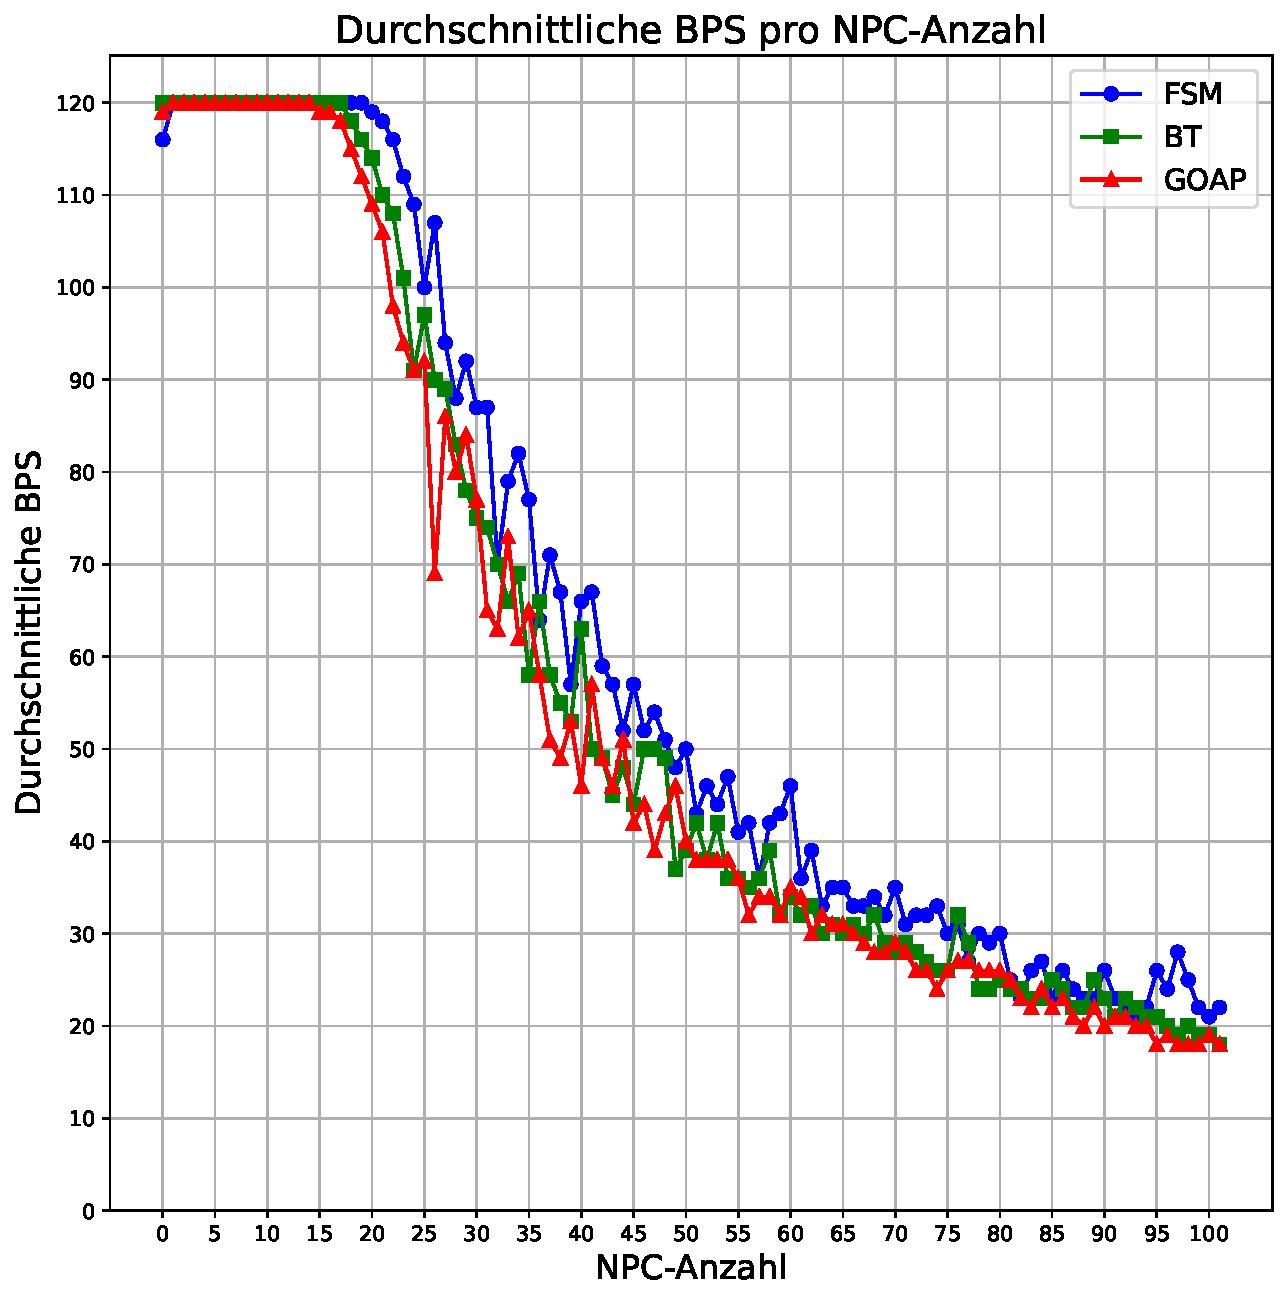
\includegraphics[width=12cm]{Vergleich/avg_fps.pdf}
	\captionsetup{justification=justified, format=plain}
  \caption{BPS-Performance Benchmark}
  \label{fig:bps benchmark}
\end{figure}

Die Abbildung \ref{fig:mem benchmark} veranschaulicht die Ergebnisse des Speicher-Benchmarks. Auch in diesem Fall erweist sich GOAP als ressourcenintensiv, jedoch bleibt der Speicherverbrauch laut dem Benchmark konstant. Es ist jedoch wichtig zu betonen, dass w\"{a}hrend der Implementierung GOAP mehrfach Speicherlecks aufgetreten sind, was auf eine h\"{o}here Empfindlichkeit dieses Systems hinweist.

\begin{figure}[h]
  \centering
  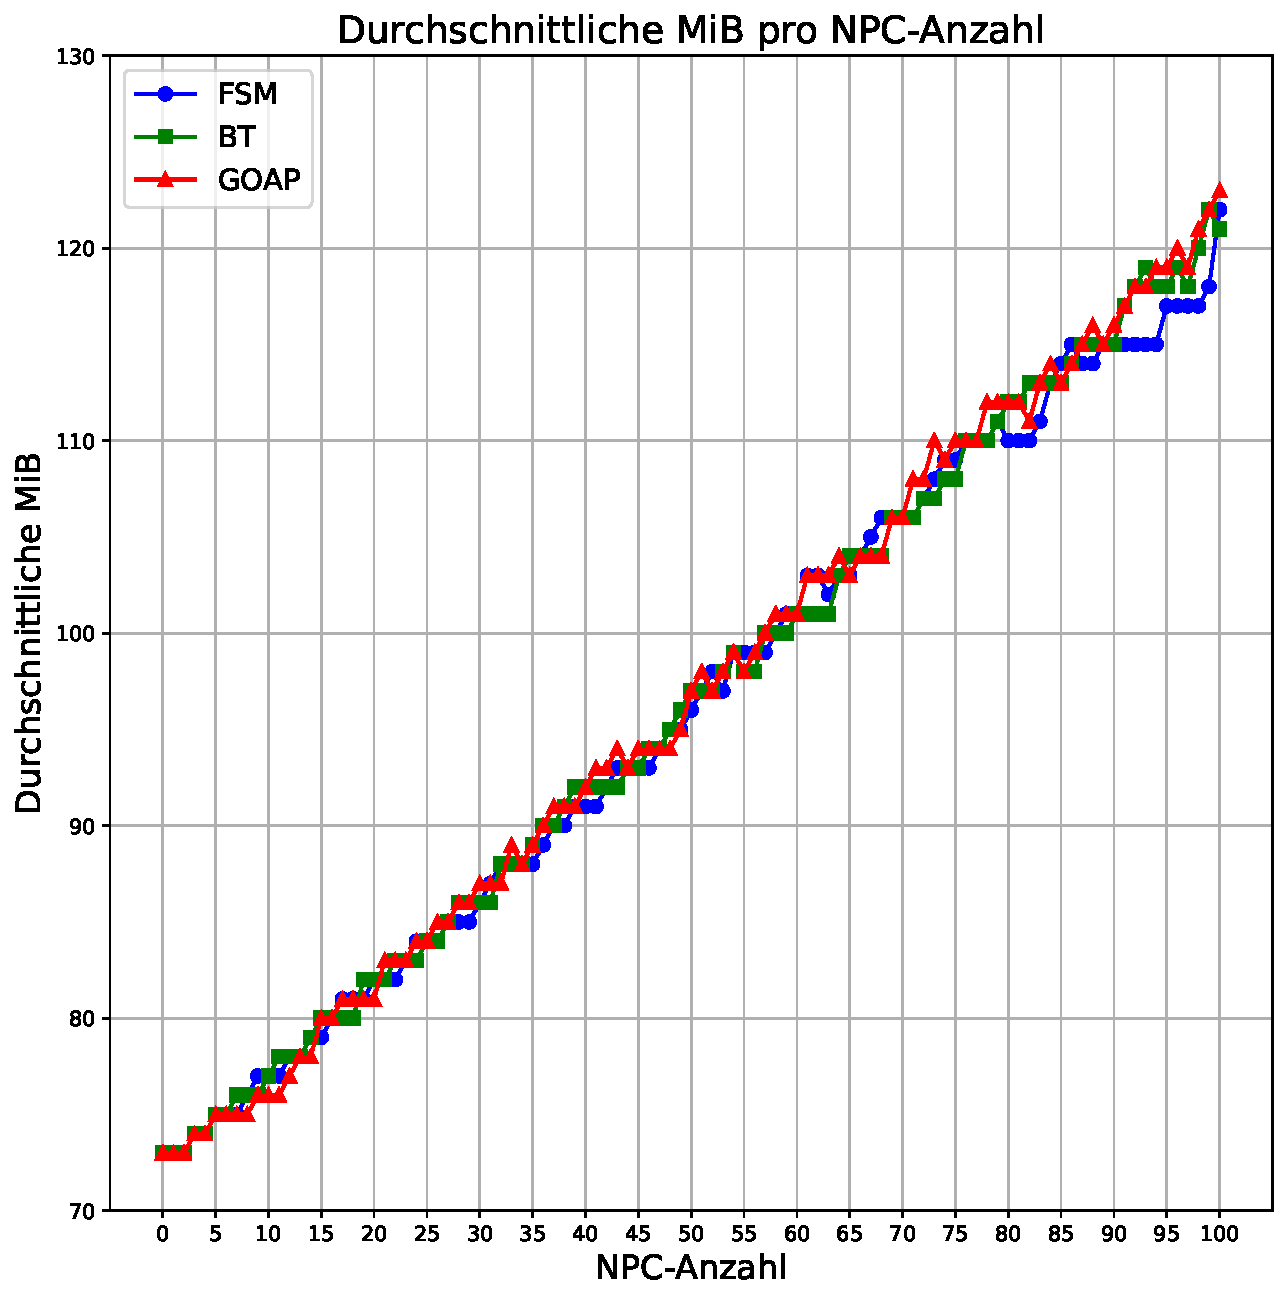
\includegraphics[width=12cm]{Vergleich/avg_mem.pdf}
	\captionsetup{justification=justified, format=plain}
  \caption{Speicher-Benchmark}
  \label{fig:mem benchmark}
\end{figure}

\section{Bewertung}
\label{chap:bewertung}

Die Wahl des Entscheidungssystems h\"{a}ngt stark von den Anforderungen des Projekts ab.

Eine FSM wird f\"{u}r einfache NPC-Logiken empfohlen. Sie ist von den anderen zwei Entscheidungssystem am einfachsten zu erlernen und in Godot umzusetzen. Will man aber komplexe NPC-Verhalten programmieren, so wird die Anzahl der Knoten wachsen, der FSM-Graph un\"{u}bersichtlicher und die Wartbarkeit wird schwieriger. Die Erweiterung durch weitere Knoten kann zur Anpassung der FSM f\"{u}hren und somit zu einem erh\"{o}hten Zeitaufwand. Das Debuggen ist jedoch durch die statische Natur der FSM vergleichsweise einfach, insbesondere wenn eine Visualisierung genutzt wird.

F\"{u}r mittlere bis komplexe NPC-Verhaltensweisen ist der BT zu empfehlen. Er ist in ihrer Funktionsweise komplexer als die FSM, hat aber viel Dokumentation zur Umsetzung, die in Godot ohne Schwierigkeiten m\"{o}glich ist. Es gibt viele Konzepte die das 
Die Skalierbarkeit und Debuggen des BT ist ebenfalls einfach.

Will man komplexe NPC-Verhalten umsetzen, so ist GOAP die beste Wahl. Mit der komplexen Funktionsweise und eher mageren Dokumentation ist es schwierig, sich einzuarbeiten. In Bezug auf Skalierbarkeit \"{u}bertrifft GOAP die anderen Systeme, da neue Aktionen unabh\"{a}ngig voneinander existieren und nicht manuell verkn\"{u}pft werden m\"{u}ssen. Dies macht GOAP besonders anpassungsf\"{a}hig. Allerdings ist das Debuggen aufgrund der dynamischen Entscheidungen schwieriger. Eine m\"{o}gliche L\"{o}sung w\"{a}re die Visualisierung des Suchbaums, jedoch ist dies deutlich aufwendiger zu implementieren als bei FSM oder BT.

Die Tabelle\ref{tab:es vergleich tabelle} veranschaulicht die abschlie\ss{}ende Bewertung der Entscheidungssysteme mithilfe von Harvey Balls. Je voller der Harvey Ball, desto besser die Bewertung. Die Bewertungen basieren auf Vergleichen und Benchmarks.


\begin{table}[h]
  \caption{Tabellarische Bewertung}
  \label{tab:es vergleich tabelle}
  \centering
  \begin{tabular}{lccc}
    \toprule
    & FSM & BT & GOAP\\
    \midrule
		Erlernbarkeit & \harveyBallFull & \harveyBallThreeQuarter & \harveyBallHalf\\
    Implementation	& \harveyBallFull  & \harveyBallThreeQuarter  & \harveyBallHalf\\
		NPC-Design & \harveyBallQuarter & \harveyBallThreeQuarter & \harveyBallFull\\
    Skalierbarkeit	& \harveyBallQuarter & \harveyBallHalf & \harveyBallFull\\
    Debugging	& \harveyBallHalf & \harveyBallThreeQuarter & \harveyBallQuarter\\
		Performance & \harveyBallFull & \harveyBallThreeQuarter & \harveyBallHalf\\
		Speicherverbrauch & \harveyBallFull & \harveyBallFull & \harveyBallThreeQuarter\\
    \bottomrule
  \end{tabular}
\end{table}
\chapter{Fazit}

\autocite{golem4}:
Die Wahl zwischen Unity und Godot h�ngt davon ab, welche Priorit�ten man setzt. Sollte man auf Sicherheit vor Lizenz�nderungen sowie Mehrkosten abzielen, so w�re Godot die Wahl. Erwartet man eine technisch ausgereifte, bew�hrtes Engine-Framework mit professionellem Support und einem prall gef�llten Asset-Store.
%\chapter{Schreibstil}

\section{Fremdsprachige Begriffe}

Wenn Sie Ihre Arbeit auf Deutsch verfassen, gehen Sie sparsam mit englischen Ausdrücken um. Natürlich brauchen Sie etablierte englische Fachbegriffe, wie z.\,B. \textit{Interrupt}, nicht zu übersetzen. Sie sollten aber immer dann, wenn es einen gleichwertigen deutschen Begriff gibt, diesem den Vorrang geben. Den englischen Begriff (\textit{term}) können Sie dann in Klammern oder in einer Fußnote\footnote{Englisch: \textit{footnote}.} erwähnen. Absolut unakzeptabel sind deutsch gebeugte englische Wörter oder Kompositionen aus deutschen und englischen Wörtern wie z.\,B. downgeloadet, upgedated, Keydruck oder Beautyzentrum.


\section{Zitate}

\subsection{Zitate im Text}

Wichtig ist das korrekte Zitieren von Quellen, wie es auch von \cite{Kornmeier2011} dargelegt wird. Interessant ist in diesem Zusammenhang auch der Artikel von \cite{Kramer2009}. Häufig werden die Zitate auch in Klammern gesetzt, wie bei \parencite{Kornmeier2011} und mit Seitenzahlen versehen \parencite[S. 22--24]{Kornmeier2011}.

Bei Webseiten wird auch die URL und das Abrufdatum mit angegeben \parencite{Gao2017}. Wenn die URL nicht korrekt umgebrochen wird, lohnt es sich, an den Parametern \textit{biburl*penalty} in der \texttt{preambel.tex} zu drehen. Kleinere Werte erhöhen die Wahrscheinlichkeit, dass getrennt wird.

\subsection{Zitierstile}

Verwenden Sie eine einheitliche und im gesamten Dokument konsequent durchgehaltene Zitierweise\index{Zitierweise}. Es gibt eine ganze Reihe von unterschiedlichen Standards für das Zitieren und den Aufbau eines Literaturverzeichnisses. Sie können entweder mit Fußnoten oder Kurzbelegen im Text arbeiten. Welches Verfahren Sie einsetzen ist Ihnen überlassen, nur müssen Sie es konsequent durchhalten.

In der Informatik ist das Zitieren mit Kurzbelegen\index{Zitat!Kurzbeleg} im Text (Harvard"=Zitierweise) weit verbreitet, wobei für das Literaturverzeichnis häufig die Regeln der \acs{ACM} oder \acs{IEEE} angewandt werden.\footnote{Einen Überblick über viele verschiedene Zitierweisen finden Sie in der \url{http://amath.colorado.edu/documentation/LaTeX/reference/faq/bibstyles.pdf}}

Am einfachsten ist es, wenn Sie das \verb+\autocite{}+-Kommando verwenden. Bei diesem Kommando können Sie in der Datei \texttt{perambel.tex} festlegen, wie die Zitate generell aussehen sollen, \zb \ ob sie in Fußnoten erfolgen sollen oder nicht. Wollen Sie von dem globalen Zitierstil abweichen, können Sie weiterhin spezielle Kommandos benutzen:

\begin{itemize}
	\item \verb+\autocite{Willberg1999}+: \autocite{Willberg1999}
	\item \verb+\cite{Willberg1999}+: \cite{Willberg1999}
	\item \verb+\parencite{Willberg1999}+: \parencite{Willberg1999}
	\item \verb+\footcite{Willberg1999}+: \footcite{Willberg1999}
	\item \verb+\citeauthor{Willberg1999}+: \citeauthor{Willberg1999}
	\item \verb+\citeauthor*{Willberg1999}+: \citeauthor*{Willberg1999}
	\item \verb+\citetitle{Willberg1999}+: \citetitle{Willberg1999}
	\item \verb+\fullcite{Willberg1999}+: \fullcite{Willberg1999}
\end{itemize}

Denken Sie daran, dass das Übernehmen einer fremden Textstelle ohne entsprechenden Hinweis auf die Herkunft in wissenschaftlichen Arbeiten nicht akzeptabel ist und dazu führen kann, dass die Arbeit nicht anerkannt wird. Plagiate\index{Plagiat!Bewertung} werden mit mangelhaft (5,0) bewertet und können weitere rechtliche Schritte nach sich ziehen.


\subsection{Zitieren von Internetquellen}

Internetquellen\index{Zitat!Internetquellen} sind normalerweise \textit{nicht} zitierfähig. Zum einen, weil sie nicht dauerhaft zur Verfügung stehen und damit für den Leser möglicherweise nicht beschaffbar sind und zum anderen, weil häufig der wissenschaftliche Anspruch fehlt.\footnote{Eine lesenswerte Abhandlung zu diesem Thema findet sich (im Internet) bei \cite{Weber2006}}

Wenn ausnahmsweise doch eine Internetquelle zitiert werden muss, z.\,B. weil für eine Arbeit dort Informationen zu einem beschriebenen Unternehmen abgerufen wurden, sind folgende Punkte zu beachten:

\begin{itemize}
\item Die Webseite ist auszudrucken und im Anhang der Arbeit beizufügen,
\item das Datum des Abrufs und die URL sind anzugeben,
\item verwenden Sie Internet"=Seiten ausschließlich zu illustrativen Zwecken (z.\,B. um einen Sachverhalt noch etwas genauer zu erläutern), aber nicht zur Faktenvermittlung (z.\,B. um eine Ihrer Thesen zu belegen).
\end{itemize}

Wenn Sie aufgrund der Natur Ihrer Arbeit sehr viele Internetquellen benötigen, dann können Sie diese statt sie auszudrucken auch in elektronischer Form abgeben (CD/DVD). Als Abgabeformat der elektronischen Quellen ist PDF/A\footnote{Bei PDF/A handelt es sich um ein besonders stabile Variante des \ac{PDF}, die von der  \ac{ISO} standardisiert wurde.} vorteilhaft, weil es von allen Formaten die größte Stabilität besitzt.
Auf der CD/DVD geben Sie bitte auch eine HTML"=Version des Literaturverzeichnisses ab, in der die Online"=Quellen sowie die gespeicherten PDF"=Dateien verlinkt sind.

Wikipedia\index{Zitat!Wikipedia} stellt einen immensen Wissensfundus dar und enthält zu vielen Themen hervorragende Artikel. Sie müssen sich aber darüber im Klaren sein, dass die Artikel in Wikipedia einem ständigen Wandel unterworfen sind und nicht als Quelle für wissenschaftliche Fakten genutzt werden sollten. Es gelten die allgemeinen Regeln für das Zitieren von Internetquellen. Sollten Sie doch Wikipedia nutzen müssen, verwenden Sie bitte ausschließlich den Perma"=Link\footnote{Sie erhalten den Permalink über die Historie der Seite und einen Klick auf das Datum.}\index{Permalink} zu der Version der Seite, die Sie aufgerufen haben.


% Jedes Kapitel besteht aus Unterkapiteln (section)
\section{Gliederung: Zweite Ebene}

Die Gliederung im Inhaltsverzeichnis erfolgt mit Kapiteln \verb+\chapter{Titel}+, Abschnitten \verb+\section{Titel}+, Unterabschnitten \verb+\subsection{Titel}+. Zusätzlich können noch Unterunterabschnitte \verb+\subsubsection{Titel}+ und Absätze \verb+\paragraph{Titel}+ verwendet werden. Damit kommt man auf maximal fünf Ebenen, was für eine Abschlussarbeit mehr als ausreichend ist.

Auf jeder Ebene sollten Sie erläutern, was in den darunter liegenden Ebene beschrieben wird, sodass im Normalfall keine Gliederungsebene leer ist und nur aus Untereinheiten besteht. Im folgenden zeigt dieses Template, wie man weitere Ebenen mit \LaTeX erzeugt.

% Unterkapitel können noch einmal durch subsections untergliedert
% werden (jetzt auf der 3. Ebene)
\subsection{Gliederung: Dritte Ebene}

% Mit Labels können Sie sich später im Text wieder auf diese Stelle beziehen
\label{Gliederung:EbeneDrei}

% Einträge für den Index anlegen. Ein Index wird normalerweise in einer Abschluss-
% arbeit nicht benötigt.
\index{Gliederung!Ebenen}

% Auf der 4. Ebene liegen die subsubsections. In diesem Template bekommt die
% 4. Ebene keinen Nummern mehr und erscheint auch nicht im Inhaltsverzeichnis.
\subsubsection{Gliederung: Vierte Ebene}

% Auf der 5. Ebene werden einzelne Absätze mit Überschriften versehen.
\paragraph{Gliederung: Fünfte Ebene} Anders als in diesem Beispiel, darf in Ihrer Arbeit kein Gliederungspunkt auf seiner Ebene alleine stehen. D.\,h. wenn es ein 1.1 gibt, muss es auch ein 1.2 geben.
 % Externe Datei einbinden
%\chapter{Typografie}

\section{Hervorhebungen}
\label{Einleitung:Textauszeichnungen}

Achten Sie bitte auf die grundlegenden Regeln der Typografie\index{Typografie}\footnote{Ein Ratgeber in allen Detailfragen ist \cite{Forssman2002}.}, wenn Sie Ihren Text schreiben. Hierzu gehören z.\,B. die Verwendung der richtigen "`Anführungszeichen"' und der Unterschied zwischen Binde- (-), Gedankenstrich (--) und langem Strich (---). Sie erhalten den Bindestrich in \LaTeX{} mit \verb+-+, den Gedankenstrich mit \verb+--+ und den langen Strich mit \verb+---+.

Wenn Sie Text hervorheben wollen, dann setzten Sie ihn mit \verb+\textit+ \textit{kursiv} (Italic) und nicht \textbf{fett} (Bold). Fettdruck ist Überschriften vorbehalten; im Fließtext stört er den Lesefluss. Das \underline{Unterstreichen} von Fließtext ist im gesamten Dokument tabu und kann maximal bei Pseudo"=Code vorkommen.\index{Hervorhebungen}


\section{Anführungszeichen}

Deutsche Anführungszeichen werden mit \verb+"`+ und \verb+"'+ erzeugt: "`dieser Text steht in \glq Anführungszeichen\grq; alles klar?"'. Englische Anführungszeichen hingegen mit \verb+``+ und \verb+''+: ``this is an `English' quotation''. Beachten Sie, dass Sie in Zitaten immer die zur Sprache passenden Anführungszeichen verwenden. Die Verwendung von \verb+"+ ist für Anführungszeichen immer falsch und führt bei \LaTeX{} zu seltsamen "Effekten".

Um sich diesen Ärger zu sparen, biete sich die Verwendung des Paketes \textit{csquotes} und des Kommandos \verb+\enquote+ an. Hierdurch werden die Anführungszeichen korrekt für die eingestellte Sprache gesetzt und Sie müssen sich \enquote{keine Sorgen mehr über die \enquote{Anführungszeichen} machen}.


\section{Silbentrennung}
\index{Silbentrennung}
\LaTeX{} führt eine automatische Silbentrennung durch, sodass Sie sich eigentlich um nichts kümmern müssen. Allerdings werden Wörter, die bereits einen Bindestrich enthalten nicht getrennt, z.\,B. Datenschutz-Grundverordnung. Wenn Sie Ihren Text auf Deutsch schreiben, können Sie dann alternativ \verb+"=+ für den Bindestrich im Wort verwenden, z.\,B. \\
\verb+Datenschutz"=Grundverordnung+, damit \LaTeX{}  weiterhin richtig trennt.

Ist die Silbentrennung aus einem anderen Grund nicht erfolgt, z.\,B. weil das Wort nur aus Großbuchstaben besteht, sodass die Zeile über den rechten Rand hinaussteht (Sie bekommen eine \textit{overfull hbox}-Warnung), können Sie \LaTeX{} helfen, indem Sie weitere Trennstellen angeben. Dies geschieht durch \verb+"-+ als Zeichen, z.\,B. \verb+Staats"-ver"-trag+.

\section{Abkürzungen}
\index{Abkürzungen}
\index{Abbreviation|see{Abkürzungen}}

Eine \gls{abk} (\verb+\gls{abk}+) wird bei der ersten Verwendung ausgeschrieben. Danach nicht mehr: \gls{abk}. Man kann allerdings mit \verb+\acrlong{abk}+ die Langform explizit anfordern (\acrlong{abk}) oder mit \verb+\acrshort{abk}+ die Kurzform (\acrshort{abk}) oder mit \verb+\acrfull{abk}+ auch noch einmal die Definition (\acrfull{abk}). Wenn Sie eine Abkürzung im Plural verwenden wollen, gibt ihnen \verb+\glspl{isp}+ die Möglichkeit (\glspl{isp}).

Das Abkürzungsverzeichnis muss aufgrund der automatischen Sortierung separat kompiliert werden. Der dazugehörige Befehl lautet:
\begin{verbatim}
makeindex -s %.ist -t %.alg -o %.acr %.acn
\end{verbatim}

Beachten Sie, dass bei Abkürzungen, die für zwei Wörter stehen, ein schmales Leerzeichen nach dem Punkt kommt (\verb+\,+ in \LaTeX{}): z.\,B. bzw. \zb{} und d.\,h. bzw. \dahe{}. Das Template bietet hierfür die beiden Makros \verb+\zb{}+ und \verb+\dahe{}+.


\section{Glossar}
Ein Eintrag in dem Glossar kann mithilfe des Befehls \verb*|\gls{glos:amplification}| erzeugt werden. Hierbei wird die Begriffserklärung in der Datei \texttt{/kapitel/glossar} verwendet und in dem Verzeichnis aufgeführt. Ein Beispiel hierfür wäre: \gls{glos:amplification}. Das Wort Amplification erscheint nun in der Begriffserklärung.

Das Glossar muss aufgrund der automatischen Sortierung separat kompiliert werden. Der dazugehörige Befehl lautet:
\begin{verbatim}
	"makeindex.exe" -s %.ist -t %.glg -o %.gls %.glo
\end{verbatim}



\section{Symbolverzeichnis}
Ein Eintrag in dem Symbolverzeichnis kann mithilfe des Befehls \verb*|\gls{symb:Pi}| erzeugt werden. Hierbei wird das Symbol in der Datei \texttt{/kapitel/symbole} geladen und in dem Verzeichnis aufgeführt. Ein Beispiel hierfür ist: \gls{symb:Pi} und \gls{symb:energyconsump}.

Das Symbolverzeichnis muss aufgrund der automatischen Sortierung separat kompiliert werden. Der dazugehörige Befehl lautet:

\begin{verbatim}
	"makeindex.exe" -s %.ist -t %.slg -o %.syi %.syg
\end{verbatim}


\section{Querverweise}

Querverweise auf eine Kapitelnummer macht man im Text mit \verb+\ref+ (Kapitel~\ref{Einleitung:Textauszeichnungen}) und auf eine bestimmte Seite mit \verb+\pageref+ (Seite~\pageref{Einleitung:Textauszeichnungen}). Man kann auch den Befehl \verb+\autoref+ benutzen, der automatisch die Art des referenzierten Elements bestimmt (\zb{} \autoref{Einleitung:Textauszeichnungen} oder \autoref{Kap2:Kopplungsformen}).


\section{Fußnoten}

Fußnoten werden einfach mit in den Text geschrieben, und zwar genau an die Stelle\footnote{An der die Fußnote auftauchen soll}. Hierzu dient der Befehl \verb+\footnote{Text}+.


\section{Tabellen}

Tabellen werden normalerweise ohne vertikale Striche gesetzt, sondern die Spalten werden durch einen entsprechenden Abstand voneinander getrennt.\footnote{Siehe \cite[S. 89]{Willberg2021}.} Zum Einsatz kommen ausschließlich horizontale Linien (siehe \autoref{Kap2:Kopplungsformen}).

\begin{table}[ht]
  \caption{Ebenen der Kopplung und Beispiele für enge und lose Kopplung}
  \label{Kap2:Kopplungsformen}
  \renewcommand{\arraystretch}{1.2}
  \small
  \centering
  \resizebox{\linewidth}{!}{ 
    \begin{tabular}{l l l}
    \toprule
    \textbf{Form der Kopplung} & \textbf{enge Kopplung} & \textbf{lose Kopplung}\\
    \midrule
    Physikalische Verbindung	&	Punkt-zu-Punkt	& 	über Vermittler\\
    Kommunikationsstil	&	synchron		&	asynchron\\
    Datenmodell	&	komplexe gemeinsame Typen	&	nur einfache gemeinsame Typen\\
    Bindung	&	statisch		&	dynamisch\\
    \bottomrule
    \end{tabular}
	}
\end{table}

Eine Tabelle fließt genauso, wie auch Bilder durch den Text. Siehe \autoref{Kap2:Kopplungsformen}.

Manchmal möchte man Tabellen, in denen der Text in der Tabellenspalte umbricht. Hierzu dient die Umgebung \texttt{tabularx}, wobei \texttt{L} eine Spalte mit Flattersatz und \texttt{X} eine mit Blocksatz definiert. Die Breite der Tabelle kann über den Faktor vor \verb+\textwidth+ angegeben werden.

\begin{table}[ht]
  \caption{Teildisziplinen der Informatik}
  \label{Kap2:Teildisziplinen}
  \renewcommand{\arraystretch}{1.2}
  \centering
  \small
    \begin{tabularx}{0.95\textwidth}{l X L}
      \toprule
      \textbf{Gebiet} & \textbf{Definition} & \textbf{Beispiel}\\
      \toprule
      \emph{Praktische Informatik} & Informatik-Disziplinen, welche sich vorwiegend mit der Entwicklung und Anwendung der Software-Komponenten befassen & Programmentwicklung, Compilerbau; im Aufbau von z.B. Informationssystemen und Netzwerken ergeben sich Überlappungen mit der technischen Informatik \\\midrule
      \emph{Technische Informatik} & Informatik-Disziplinen, welche sich vorwiegend mit der Entwicklung und Anwendung der Hardware-Komponenten befassen & Digitaltechnik, Mikroprozessortechnik \\\midrule
      \emph{Theoretische Informatik} & Informatik-Disziplinen, welche sich mit der Entwicklung von Theorien und Modellen der Informatik befassen und dabei viel Substanz aus der Mathematik konsumieren & Relationenmodell, Objekt-Paradigmen, Komplexitätstheorie, Kalküle \\\midrule
      \emph{Angewandte Informatik} & Informatik als instrumentale Wissenschaft & Rechtsinformatik, Wirtschaftsinformatik, Geoinformatik \\
      \bottomrule
    \end{tabularx}
\end{table}

Manchmal kommt es vor, dass eine Tabelle so lang wird, dass sie sich über mehr als eine Seite erstreckt. In diesem Fall können Sie das Paket \texttt{longtable} verwenden und die Tabelle mit \verb+\begin{longtable}[h]+ definieren. Die Tabelle wird dann \textit{nicht} in eine \texttt{table}-Umgebung eingeschlossen. Siehe hierzu \autoref{laendercodes} in \autoref{AnhangA}.


\section{Harveyballs}

\begin{quote}
    Harvey Balls sind kreisförmige Ideogramme, die dazu dienen, qualitative Daten anschaulich zu machen. Sie werden in Vergleichstabellen verwendet, um anzuzeigen, inwieweit ein Untersuchungsobjekt sich mit definierten Vergleichskriterien deckt. \parencite{Wikipedia_HarveyBalls}
\end{quote}

\begin{table}[ht]
  \caption{Beispiel für Harvey Balls}
  \label{tab:harveyexample}
  \centering
  \begin{tabular}{lccc}
    \toprule
    & Ansatz 1 & Ansatz 2 & Ansatz 3\\
    \midrule
    Eigenschaft 1	& \harveyBallNone & \harveyBallQuarter & \harveyBallHalf \\
    Eigenschaft 2	& \harveyBallHalf & \harveyBallThreeQuarter & \harveyBallFull \\
    Eigenschaft 3	& \harveyBallFull & \harveyBallThreeQuarter & \harveyBallQuarter\\
    \bottomrule
  \end{tabular}
\end{table}


\section{Aufzählungen}

Aufzählungen sind toll.

\begin{itemize}
  \item Ein wichtiger Punkt
  \item Noch ein wichtiger Punkt
  \item Ein Punkt mit Unterpunkten
    \begin{itemize}
      \item Unterpunkt 1
      \item Unterpunkt 2
    \end{itemize}
  \item Ein abschließender Punkt ohne Unterpunkte
\end{itemize}


Aufzählungen mit laufenden Nummern sind auch toll.

\begin{enumerate}
  \item Ein wichtiger Punkt
  \item Noch ein wichtiger Punkt
  \item Ein Punkt mit Unterpunkten
    \begin{enumerate}
      \item Unterpunkt 1
      \item Unterpunkt 2
    \end{enumerate}
  \item Ein abschließender Punkt ohne Unterpunkte
\end{enumerate}


Aufzählungen mit eigenen Bezeichnern sind auch toll.
\begin{enumerate}[label=RQ~\arabic*), leftmargin=1.75cm]
	\item Ein wichtiger Punkt
	\item Noch ein wichtiger Punkt
	\item Ein Punkt mit Unterpunkten
	\item Ein abschließender Punkt ohne Unterpunkte
\end{enumerate}


Auch die Auflistung im Fließtext ist sehr wertvoll: \begin{enumerate*}[label=\alph *)] \item wichtiger Punkt, \item zweiter wichtiger Punkt und \item der letzte Punkt. \end{enumerate*}


 % Externe Datei einbinden
%\chapter{Einbinden von Grafiken und Sourcecode}
\label{Kap3}

\section{Bilder}

Natürlich können auch Grafiken und Bilder eingebunden werden, siehe z.\,B. Abbildung~\ref{Kap2:NasaRover}.

\begin{figure}[h]
  \centering
  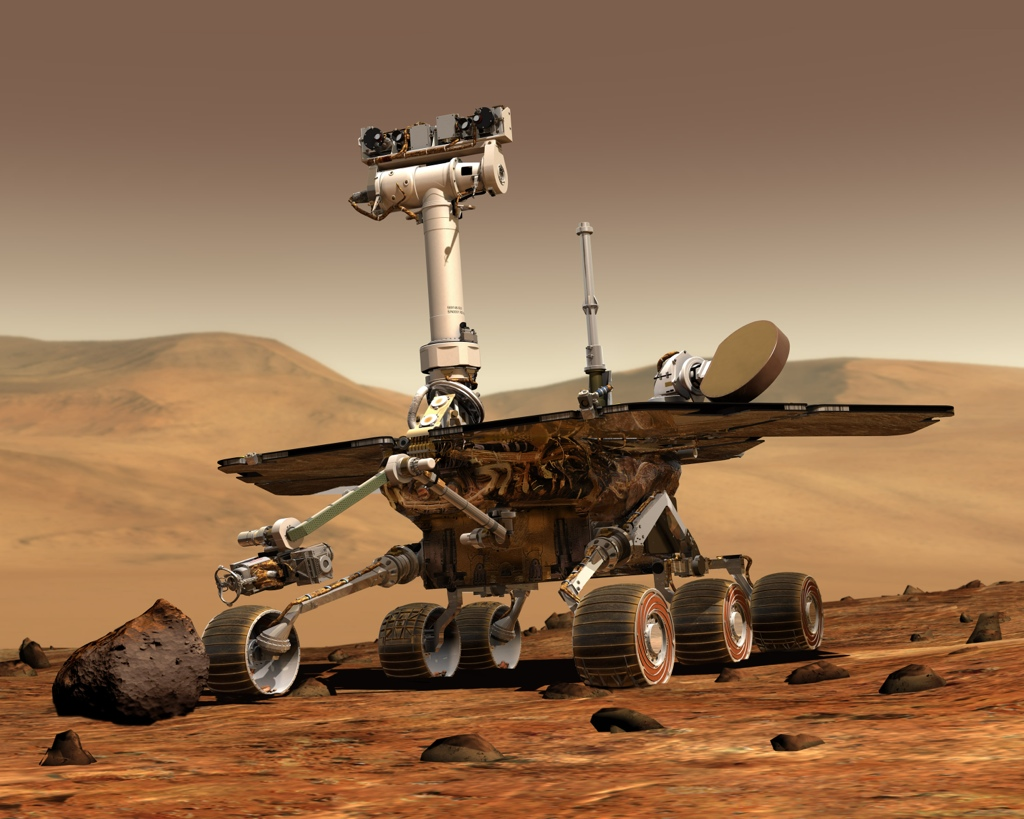
\includegraphics[width=6cm]{kapitel3/nasa_rover}
  \caption{Ein Nasa Rover}
  \label{Kap2:NasaRover}
\end{figure}


Man kann sich auch selber ein Makro für das Einfügen von Bildern schreiben:

\bild{kapitel3/modell_point_to_point}{6cm}{Point to Point}

\begin{sidewaysfigure}
 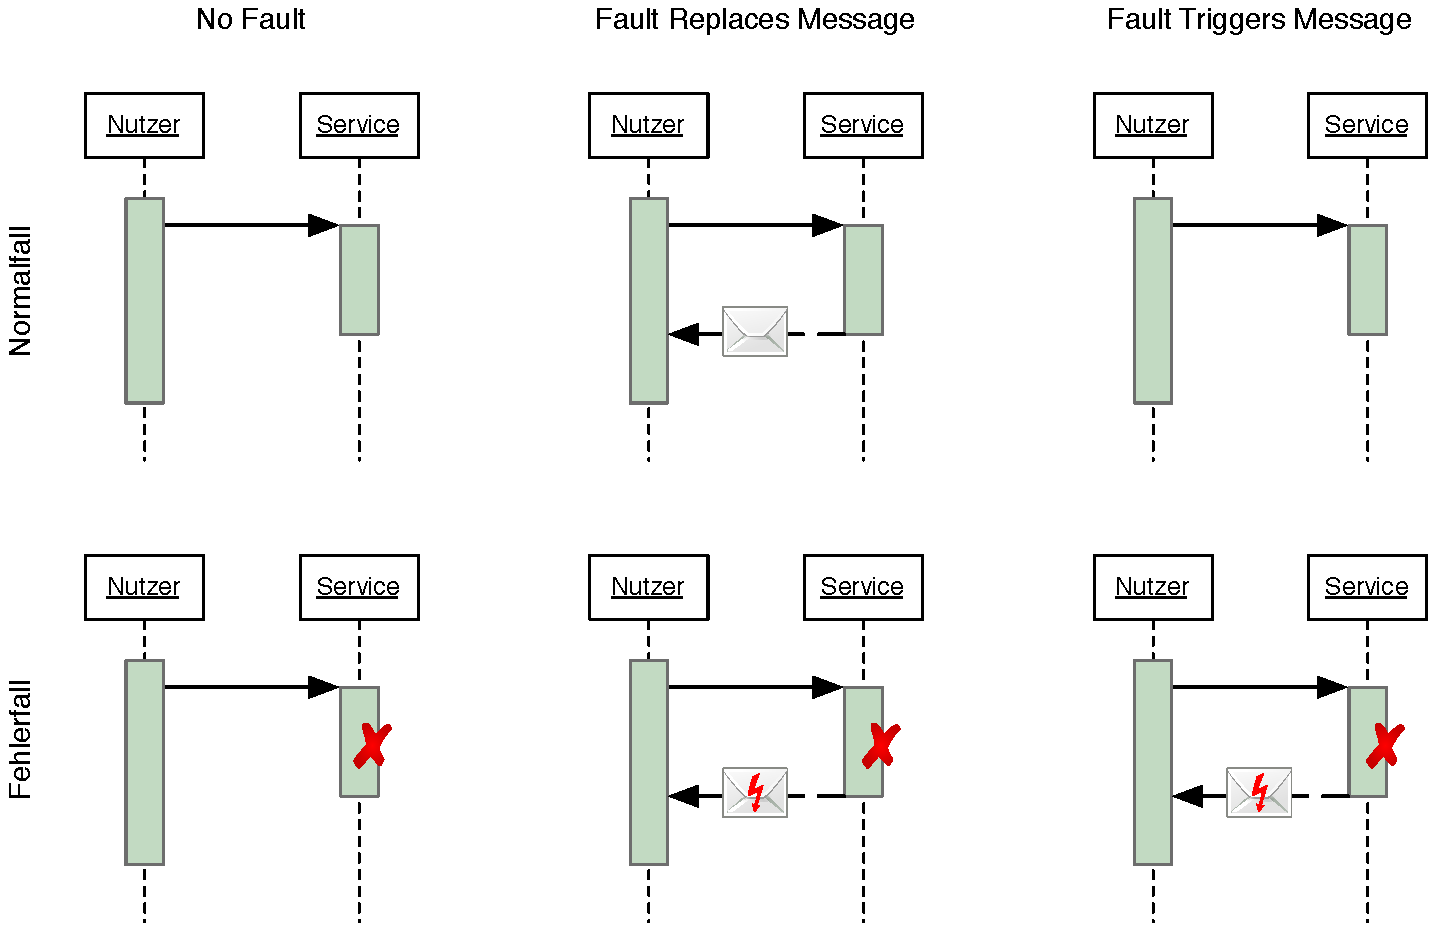
\includegraphics[width=22cm]{kapitel3/ws-wsdl20-fehler}
  \caption{Sehr große Grafiken kann man drehen, damit sie auf die Seite passen}
  \label{Kap2:wsdl-fehler}
\end{sidewaysfigure}


\clearpage % Alle Bilder, die bisher kamen ausgeben

\section{Formelsatz}

Eine Formel gefällig? Mitten im Text $a_2 = \sqrt{x^3}$ oder als eigener Absatz (siehe Formel~\ref{Formel}):

\begin{equation}
\begin{bmatrix}         
   1 &  4 &  2 \\
   4 &  0 & -3 
\end{bmatrix}        
        \cdot
\begin{bmatrix}                
   1 &  1 &  0 \\
  -2 &  3 &  5 \\
   0 &  1 &  4 
\end{bmatrix}        
       {=} 
\begin{bmatrix}               
  -7 &  15 &  28 \\
   4 &   1 & -12 
\end{bmatrix}
\label{Formel}
\end{equation}


\section{Sourcecode}

Man kann mit Latex auch ganz toll Sourcecode in den Text aufnehmen.

\subsection{Aus einer Datei}

\lstinputlisting[firstline=2,language=Java,caption={Crypter-Interface},label=lst:CrypterInterface]{\srcloc/Crypter.java}


\subsection{Inline}

\begin{lstlisting}[language=Java,caption=Methode checkKey()]
    /**
     * Testet den Schlüssel auf Korrektheit: Er muss mindestens die Länge 1
     * haben und darf nur Zeichen von A-Z enthalten.
     *
     * @param key zu testender Schlüssel
     * @throws CrypterException wenn der Schlüssel nicht OK ist.
     */
    protected void checkKey(Key key) throws CrypterException {

        // Passt die Länge?
        if (key.getKey().length == 0) {
            throw new CrypterException("Der Schlüssel muss mindestens " +
                    "ein Zeichen lang sein");
        }

        checkCharacters(key.getKey(), ALPHABET);
    }
\end{lstlisting}


\section{Anforderungen}

Anforderungen im Format des Volere-Templates (Snowcards) \autocite{Volere} können per Makro eingefügt werden.

\snowcard % Snowcard einbinden (Anpassungen in titelblatt.tex)
   {F52} % Nummer des Requirements
   {F} % Art
   {Hoch} % Priorität
   {User Authentifizierung} % Titel
   {Interview mit Abteilungsleiter} % Herkunft (Optional)
   {F12} % Konflikte (Optional)
   {Der Benutzer ist in der Lage sich über seinen
    Benutzernamen und sein Passwort am System anzumelden} % Beschreibung
   {Ein Benutzer kann sich mit seinem Firmenweiten Benutzernamen und
   Passwort über die Anmeldemaske anmelden und hat Zugriff auf die
   Funktionen des Systems} % Fit-Kriterium (Optional)
   {Benutzerhandbuch des Altsystems} % Material (Optional)

Ebenso nicht-funktionale Anforderungen mit Hilfe von Quality Attribute Scenarios. Siehe hierzu \autocite{Barbacci2003}.

\qas % Quality-Attribute Scenario einbinden (Anpassungen in titelblatt.tex)
   {NF11} % Nummer des Requirements
   {Hoch} % Priotität
   {Performance des Jahresabschlusses} % Titel
   {Endbenutzer} % Quelle
   {Startet einen Jahresabschluss} % Stimulus
   {Buchhaltungssystem} % Artefakt
   {Das System befindet sich im normalen Betriebszustand} % Umgebung
   {Jahresabschluss ist durchgeführt und kann als PDF abgerufen werden} % Antwort
   {10 Minuten} % Antwort-Maß
 % Externe Datei einbinden
%\chapter{Checkliste}
\label{Kap4}

Die folgende Checkliste kann dazu dienen, die Arbeit auf die wichtigsten Bewertungskriterien zu prüfen. Jeder Dozent hat andere Kriterien, die unten aufgeführten dürften aber für die meisten Dozenten gültig sein.

\section{Form und Sprache}

\begin{checklist}
  \footnotesize
  \item \textbf{Aufbau}: Die Arbeit ist nach wissenschaftlichen Prinzipien aufgebaut (wesentliche Teile vorhanden, Nummerierung/Verweise korrekt, Verzeichnisse vorhanden).
    \begin{checklist}
        \item \textit{Wesentliche Teile}: Die folgenden Elemente der Arbeit sind vorhanden: Titelblatt, Abstract/Zusammenfassung, Einleitung, Hauptteil, Fazit/Ausblick.
        \item \textit{Nummerierung/Verweise}: Das Nummerierungsschema wird konsistent über die gesamte Arbeit durchgehalten, die Verweise auf die verschiedenen Elemente (Abbildungen, Tabellen etc.) sind korrekt.
        \item \textit{Verzeichnisse}: Die Arbeit enthält alle relevanten Verzeichnisse: Inhaltsverzeichnis, Literaturverzeichnis, Abbildungsverzeichnis, Tabellenverzeichnis, eventuell Glossar.
    \end{checklist}
  \item \textbf{Sprache}: Die verwendete Sprache entspricht wissenschaftlichen Ansprüchen.
    \begin{checklist}
        \item \textit{Begriffe und Definitionen}: Begriffe werden einheitlich und konsistent verwendet. Neue Begriffe werden definiert und mit Literatur hinterlegt.
        \item \textit{Abkürzungen}: Alle Abkürzungen werden eingeführt und erläutert. Abkürzungen werden bei der ersten Verwendung ausgeschrieben und in einem Abkürzungsverzeichnis geführt. Es werden keine unüblichen oder selbst erfunden Abkürzungen verwendet. Ein Glossar kann verwendet werden, um Begriffe noch einmal kompakt darzustellen.
        \item \textit{Rechtschreibung}: Die Arbeit ist frei von Rechtschreibungs-, Zeichensetzungs- und Grammatikfehlern.
    \end{checklist}
  \item \textbf{Formatierung, Typografie}: Die Formatierung der Arbeit ist korrekt und aus typographischer Sicht einwandfrei. \textit{Wenn Sie dieses Template korrekt verwenden, sollte dieser Punkt automatisch durch die Verwendung von \LaTeX \ erledigt sein.}
    \begin{checklist}
        \item \textit{Korrekte Typografie}: Schriftarten werden korrekt verwendet (nicht mehr als 2 Fonts), der Zeilenabstand ist passend, die Ränder sind ausreichend, der Satz ist korrekt.
        \item \textit{Satz von Abbildungen, Tabellen etc.}: Abbildungen sind in der richtigen Auflösung dargestellt, die Tabellen sind korrekt gesetzt, mathematische Formeln und Symbole sind sauber dargestellt.
    \end{checklist}
  \item \textbf{Abbildungen}: Abbildungen werden in ausreichendem Umfang zur Förderung des Verständnisses eingesetzt. Sie werden korrekt im Text referenziert und sind, wo immer möglich, in einer Standardnotation erstellt.
    \begin{checklist}
        \item \textit{Ausreichende Verwendung}: Komplizierte Sachverhalte werden durch Abbildungen verdeutlicht. Es werden genug Abbildungen eingesetzt, um die wichtigsten Sachverhalte zu erklären.
        \item \textit{Verständnisförderung}: Abbildungen dienen nicht als Schmuck, sondern um komplizierte Sachverhalte zu verdeutlichen.
        \item \textit{Einbindung in den Text}: Der Text muss auch ohne Abbildungen verständlich sein, die Abbildungen helfen Sachverhalte aus dem Text besser darzustellen. Der Text referenziert die Abbildung korrekt.
        \item \textit{Standardnotation, Legende}: Die Abbildungen verwenden Standard"=Notationen wie UML, FMC etc. Wo keine Standardnotation eingesetzt wird, ist eine Legende vorhanden, um die Bildelemente zu erläutern.
    \end{checklist}
  \item \textbf{Zitate}: Quellen werden konsistent nach einer gängigen Zitierweise zitiert und sind vollständig im Literaturverzeichnis angegeben.
    \begin{checklist}
        \item \textit{Zitierweise}: Die Zitierweise in der gesamten Arbeit folgt einem einheitlichen Schema, z.B. IEEE, DIN, Chicago.
        \item \textit{Vollständigkeit}: Alle Zitate sind als solche kenntlich gemacht und die Quelle wird vollständig angegeben, und Plagiate werden vermieden.
    \end{checklist}
  \item \textbf{Schreibstil}: Lebendiger, wissenschaftlicher und verständlicher Schreibstil.
    \begin{checklist}
        \item \textit{Wissenschaftlichkeit}: Der Text ist im Präsenz geschrieben, es wird die dritte Person verwendet, Fachausdrücke werden korrekt verwendet, Fremdwörter und Amerikanismen werden richtig eingesetzt.
        \item \textit{Verständlichkeit}: Abschweifungen und Wiederholungen werden vermieden, statt dessen werden präzise und übersichtliche Sätze verwendet.
        \item \textit{Lebendigkeit}: Der Text der Arbeit zeichnet sich durch eine gute Wortwahl, Sprachbilder, einen angemessenen Satzbau und eine hohe Variabilität aus.
    \end{checklist}
\end{checklist}

\section{Inhalt}

\begin{checklist}
  \footnotesize
  \item \textbf{Gliederung}: Die Gliederung ist vollständig, konsistent und sachlogisch mit angemessener Struktur und Tiefe.
    \begin{checklist}
        \item \textit{Konsistenz und Vollständigkeit}: Auf einer Ebene stehen keine Punkte alleine, die Gliederungspunkte orientieren sich an der Argumentationskette.
        \item \textit{Angemessene Tiefe}: Die Größe der einzelnen Unterpunkte ist vom Umfang her ähnlich. Es gibt keine Gliederungspunkte, die nur aus ein bis zwei Sätzen bestehen.
    \end{checklist}
  \item \textbf{Grundlagen}: Es werden alle relevanten Grundlagen gelegt. Der State"=of"=the"=art und der State"=of"=practice werden dargelegt.
    \begin{checklist}
        \item \textit{Umfang}: 1/3 des Hauptteils ist ein gutes Maß für eine ausreichende Darstellung der Grundlagen.
        \item \textit{Begriffe und Methoden}: Begriffe und Methoden sind definiert, und Literatur zu den Definitionen ist angegeben.
        \item \textit{State-of-the-art}: Der Stand des verfügbaren Wissens wird dargestellt, analysiert und kritisch beurteilt (state-of-the-art). Bei theoretischen Arbeiten kann ein eigenes Kapitel \enquote{verwandte Arbeiten} nötig sein, um den state"=of"=the"=art darzustellen.
        \item \textit{State-of-practice}: Bei praktischen Arbeiten, die in der Industrie geschrieben werden, kann es nötig sein, auch das Vorgehen im Unternehmen zu erläutern.
    \end{checklist}
  \item \textbf{Methodik/Lösung}: Die gewählte Methodik bzw. Lösung ist für das Problem adäquat.
    \begin{checklist}
        \item \textit{Anforderungen an die Lösung}: Die von der Lösung zu erfüllenden Anforderungen werden dargestellt. Wo nötig wird dies auf Grundlage eines sauberen Requirements"=Engineerings durchgeführt.
        \item \textit{Erläuterung des Lösungsansatzes}: Der gewählte Lösungsansatz wird ausführlich erläutert und verständlich dargestellt.
        \item \textit{Eignung zur Lösung der Aufgabe}: Die gewählte Lösung ist geeignet, um das beschriebene Problem zu lösen.
        \item \textit{Hypothesen}: Es sind ggf. Hypothesen gebildet worden; diese sind erläutert, und es sind Kriterien identifiziert worden, mit deren Hilfe man die Hypothesen falsifizieren kann.
        \item \textit{Alternativen}: Es werden Alternativen zur vorgeschlagenen Lösung diskutiert. Die eigene Lösung wird nicht als einzige mögliche dargestellt, sondern es werden auch andere mögliche Lösungen vorgestellt und bewertet.
        \item \textit{Begründung}: Alternativen und Kriterien für die Auswahl dieser Lösung werden dargestellt.
        \item \textit{Vorteile der Lösung}: Es wird dargestellt, wieso die entwickelte Lösung vorteilhafter ist als die bisherigen Ansätze. Diese Darstellung erfolgt auf Basis des Lösungsansatzes. Eine konkrete Validierung der Implementierung erfolgt ggf. in späteren Kapiteln.
    \end{checklist}
  \item \textbf{Logik der Argumentationskette}: Die Argumentation ist logisch und nachvollziehbar. Sie ist frei von logischen Fehlschlüssen.
  \item \textbf{Implementierung}: Wenn eine Implementierung der Lösung erfolgt, so wird die Implementierung beschrieben. Die Darstellung der Implementierung kann knapp ausfallen. Wichtig ist der Lösungsansatz, nicht die konkrete Umsetzung.
  \item \textbf{Validierung}: Die vorgeschlagene Lösung wird ggf. empirisch verprobt.
    \begin{checklist}
        \item \textit{Vorgehensweise}: Die Vorgehensweise zur Validierung der Lösung / Hypothesen ist beschrieben und geeignet, relevante Aspekte der Lösung zu überprüfen.
        \item \textit{Empirische Analyse}: Die Erfassungsmethode wird dargestellt und die Daten werden nach den Grundsätzen ordnungsgemäßer Laborpraxis gesammelt und statistisch korrekt ausgewertet.
        \item \textit{Verprobung}: Die Lösung wird an einem praktischen Beispiel verprobt, und es werden wissenschaftlich korrekte Schlüsse aus der Anwendung gezogen.
        \item \textit{Zielerreichung}: Funktioniert die gewählte Lösung nach der Implementierung? Wie weit wurde das Ziel erreicht? Falls nicht, gibt es nachvollziehbare Gründe dafür und wurden diese dargestellt?
    \end{checklist}
  \item \textbf{Diskussion}: Die Lösung und ihre Validierung wird kritisch und im Kontext möglicher Alternativen diskutiert und bewertet.
    \begin{checklist}
        \item \textit{Kritische Reflexion}: Grenzen und Schwächen der eigenen Ergebnisse werden beleuchtet.
        \item \textit{Ableitung von Konsequenzen}: Die Konsequenzen aus den Ergebnissen für die Wissenschaft und Praxis sind beschrieben.
    \end{checklist}
  \item \textbf{Quellenarbeit}: Es werden hochwertige Quellen in ausreichendem Umfang genutzt und kritisch hinterfragt. Eventuell vorhandene Quellen aus dem Unternehmen werden ebenfalls berücksichtigt.
    \begin{checklist}
        \item \textit{Umfang}: Der Umfang an Quellen richtet sich stark nach Thema und Art der Arbeit. Bei einer Bachelorarbeit sind mindestens 20 Primärquellen und entsprechend viele Sekundärquellen üblich, bei einer Masterarbeit deutlich mehr.
        \item \textit{Wissenschaftliche Qualität}: Nicht zitierfähig sind Internet"=Quellen, Wikipedia"=Einträge sowie andere Bachelor- oder Masterarbeiten (sofern nicht veröffentlicht). Das ausschließliche Zitieren von Lehrbüchern ist problematisch. Aktuelle wissenschaftliche Artikel und Werke sollten in den Quellen auftauchen.
        \item \textit{Quellen \enquote{aus der Praxis}}: Wenn es im Unternehmen spezielle Quellen und Informationen gibt, so werden diese berücksichtigt, z. B. firmen- oder branchenspezifischer Informationen.
        \item \textit{Kritische Würdigung}: Quellen und Zitate werden kritisch hinterfragt und nicht einfach unreflektiert übernommen. Es gibt eine kritische Distanz bei der Quellenauswahl und Quellenauswertung.
    \end{checklist}
  \item \textbf{Fazit}: Es wird eine Zusammenfassung der Arbeit sowie Ausblick auf weitere mögliche Arbeiten im Themenfeld gegeben, etwa die Lösung ausstehender Probleme oder die Erfüllung zusätzlicher Anforderungen.
  \item \textbf{Umfang der Arbeit}: Richtgrößen: Bachelorarbeiten: 50--80 Seiten, Masterarbeiten: 60--100 Seiten, jeweils ohne Verzeichnisse und Anhang.
\end{checklist}

\section{Vor der Abgabe}

\begin{checklist}
  \footnotesize
  \item \textit{Korrektur}: Haben Sie einen Dritten die Arbeit lesen lassen und alle gefundenen Rechtschreib- und Zeichensetzungsfehler behoben?
  \item \textit{Literaturverzeichnis}: Sind im Literaturverzeichnis irrelevante Informationen entfernt? Beispielsweise bei Büchern unnötige Informationen über die Herkunft bei Google-Books oder bei Papern doppelte Angaben der DOI?
  \item \textbf{Abgabe auf Papier}
  \begin{checklist}
    \item \textit{Template passend eingestellt}: Haben Sie in der Datei \texttt{thesis.tex} eingestellt, dass Sie auf Papier abgeben wollen?
    \item \textit{Doppel- oder einseitiger Druck}: Entspricht die Einstellung des Templates dem Druck, d.\,h. ist das Template für doppelseitigen Druck eingestellt, wenn doppelseitig gedruckt werden soll und umgekehrt?
    \item \textit{Umschläge}: Sind die Umschläge vorhanden, um die Arbeit später zu binden? Die Umschläge können in der Hausdruckerei der Hochschule erworben werden.
    \item \textit{Copyshop}: Wissen Sie, wo Sie die Arbeit drucken werden? Die Hausdruckerei kann Ihre Arbeit nicht drucken.
    \item \textit{Exemplare}: Haben Sie geklärt, ob der Zweitkorrektor auch ein gedrucktes Exemplar möchte?
  \end{checklist}
  \item \textbf{Digitale Abgabe}
  \begin{checklist}
    \item \textit{Zustimmung des Betreuers/der Betreuerin}: Haben Sie mit Ihrer Betreuerin bzw. Ihrem Betreuer abgeklärt, dass Sie digital abgeben dürfen?
    \item \textit{Template passend eingestellt}: Haben Sie in der Datei \texttt{thesis.tex} eingestellt, dass Sie digital abgeben wollen?
    \item \textit{Unterschrift}: Haben Sie Ihre Unterschrift eingescannt und unter dem Namen \texttt{unterschrift.png} im Hauptverzeichnis abgelegt?
  \end{checklist}
\end{checklist}
 % Externe Datei einbinden


\label{lastpage}
%Beginn des Anhangs. Befehl \appendix nicht entfernen auch wenn kein Anhang vorhanden ist!
\appendix
\chapter{Erster Anhang: Lange Tabelle}
\label{AnhangA}

Hier ein Beispiel für einen Anhang. Der Anhang kann genauso in Kapitel und Unterkapitel unterteilt werden, wie die anderen Teile der Arbeit auch.

\sffamily
\begin{footnotesize}
  \begin{longtable}[c]{ p{.5\textwidth} p{.1\textwidth} p{.1\textwidth} p{.1\textwidth}}
    \caption[Tabelle mit ISO-Ländercodes]                       % Caption für das Tabellenverzeichnis
        {Lange Tabelle mit ISO-Ländercodes\label{laendercodes}} % Caption für die Tabelle selbst
        \\
    \toprule
    \textbf{Country} & \textbf{A 2} & \textbf{A 3} & \textbf{Number} \\
    \midrule
    AFGHANISTAN                                    & AF & AFG & 004 \\
    ALBANIA                                        & AL & ALB & 008 \\
    ALGERIA                                        & DZ & DZA & 012 \\
    AMERICAN SAMOA                                 & AS & ASM & 016 \\
    ANDORRA                                        & AD & AND & 020 \\
    ANGOLA                                         & AO & AGO & 024 \\
    ANGUILLA                                       & AI & AIA & 660 \\
    ANTARCTICA                                     & AQ & ATA & 010 \\
    ANTIGUA AND BARBUDA                            & AG & ATG & 028 \\
    ARGENTINA                                      & AR & ARG & 032 \\
    ARMENIA                                        & AM & ARM & 051 \\
    ARUBA                                          & AW & ABW & 533 \\
    AUSTRALIA                                      & AU & AUS & 036 \\
    AUSTRIA                                        & AT & AUT & 040 \\
    AZERBAIJAN                                     & AZ & AZE & 031 \\
    BAHAMAS                                        & BS & BHS & 044 \\
    BAHRAIN                                        & BH & BHR & 048 \\
    BANGLADESH                                     & BD & BGD & 050 \\
    BARBADOS                                       & BB & BRB & 052 \\
    BELARUS                                        & BY & BLR & 112 \\
    BELGIUM                                        & BE & BEL & 056 \\
    BELIZE                                         & BZ & BLZ & 084 \\
    BENIN                                          & BJ & BEN & 204 \\
    BERMUDA                                        & BM & BMU & 060 \\
    BHUTAN                                         & BT & BTN & 064 \\
    BOLIVIA                                        & BO & BOL & 068 \\
    BOSNIA AND HERZEGOWINA                         & BA & BIH & 070 \\
    BOTSWANA                                       & BW & BWA & 072 \\
    BOUVET ISLAND                                  & BV & BVT & 074 \\
    BRAZIL                                         & BR & BRA & 076 \\
    BRITISH INDIAN OCEAN TERRITORY                 & IO & IOT & 086 \\
    BRUNEI DARUSSALAM                              & BN & BRN & 096 \\
    BULGARIA                                       & BG & BGR & 100 \\
    BURKINA FASO                                   & BF & BFA & 854 \\
    BURUNDI                                        & BI & BDI & 108 \\
    CAMBODIA                                       & KH & KHM & 116 \\
    CAMEROON                                       & CM & CMR & 120 \\
    CANADA                                         & CA & CAN & 124 \\
    CAPE VERDE                                     & CV & CPV & 132 \\
    CAYMAN ISLANDS                                 & KY & CYM & 136 \\
    CENTRAL AFRICAN REPUBLIC                       & CF & CAF & 140 \\
    CHAD                                           & TD & TCD & 148 \\
    CHILE                                          & CL & CHL & 152 \\
    CHINA                                          & CN & CHN & 156 \\
    CHRISTMAS ISLAND                               & CX & CXR & 162 \\
    COCOS (KEELING) ISLANDS                        & CC & CCK & 166 \\
    COLOMBIA                                       & CO & COL & 170 \\
    COMOROS                                        & KM & COM & 174 \\
    CONGO                                          & CG & COG & 178 \\
    COOK ISLANDS                                   & CK & COK & 184 \\
    COSTA RICA                                     & CR & CRI & 188 \\
    COTE D'IVOIRE                                  & CI & CIV & 384 \\
    CROATIA (local name: Hrvatska)                 & HR & HRV & 191 \\
    CUBA                                           & CU & CUB & 192 \\
    CYPRUS                                         & CY & CYP & 196 \\
    CZECH REPUBLIC                                 & CZ & CZE & 203 \\
    DENMARK                                        & DK & DNK & 208 \\
    DJIBOUTI                                       & DJ & DJI & 262 \\
    DOMINICA                                       & DM & DMA & 212 \\
    DOMINICAN REPUBLIC                             & DO & DOM & 214 \\
    EAST TIMOR                                     & TP & TMP & 626 \\
    ECUADOR                                        & EC & ECU & 218 \\
    EGYPT                                          & EG & EGY & 818 \\
    EL SALVADOR                                    & SV & SLV & 222 \\
    EQUATORIAL GUINEA                              & GQ & GNQ & 226 \\
    ERITREA                                        & ER & ERI & 232 \\
    ESTONIA                                        & EE & EST & 233 \\
    ETHIOPIA                                       & ET & ETH & 210 \\
    FALKLAND ISLANDS (MALVINAS)                    & FK & FLK & 238 \\
    FAROE ISLANDS                                  & FO & FRO & 234 \\
    FIJI                                           & FJ & FJI & 242 \\
    \bottomrule
  \end{longtable}
\end{footnotesize}
\rmfamily


\textit{Beachten Sie, dass die Tabelle manchmal erst nach dreimaligem Lauf durch \LaTeX richtig angezeigt wird.}

%Wenn Sie keinen Anhang haben, entfernen Sie ausschlie\ss{}lich die nachfolgenden beiden Dateien.
%\chapter{Erster Anhang: Lange Tabelle}
\label{AnhangA}

Hier ein Beispiel für einen Anhang. Der Anhang kann genauso in Kapitel und Unterkapitel unterteilt werden, wie die anderen Teile der Arbeit auch.

\sffamily
\begin{footnotesize}
  \begin{longtable}[c]{ p{.5\textwidth} p{.1\textwidth} p{.1\textwidth} p{.1\textwidth}}
    \caption[Tabelle mit ISO-Ländercodes]                       % Caption für das Tabellenverzeichnis
        {Lange Tabelle mit ISO-Ländercodes\label{laendercodes}} % Caption für die Tabelle selbst
        \\
    \toprule
    \textbf{Country} & \textbf{A 2} & \textbf{A 3} & \textbf{Number} \\
    \midrule
    AFGHANISTAN                                    & AF & AFG & 004 \\
    ALBANIA                                        & AL & ALB & 008 \\
    ALGERIA                                        & DZ & DZA & 012 \\
    AMERICAN SAMOA                                 & AS & ASM & 016 \\
    ANDORRA                                        & AD & AND & 020 \\
    ANGOLA                                         & AO & AGO & 024 \\
    ANGUILLA                                       & AI & AIA & 660 \\
    ANTARCTICA                                     & AQ & ATA & 010 \\
    ANTIGUA AND BARBUDA                            & AG & ATG & 028 \\
    ARGENTINA                                      & AR & ARG & 032 \\
    ARMENIA                                        & AM & ARM & 051 \\
    ARUBA                                          & AW & ABW & 533 \\
    AUSTRALIA                                      & AU & AUS & 036 \\
    AUSTRIA                                        & AT & AUT & 040 \\
    AZERBAIJAN                                     & AZ & AZE & 031 \\
    BAHAMAS                                        & BS & BHS & 044 \\
    BAHRAIN                                        & BH & BHR & 048 \\
    BANGLADESH                                     & BD & BGD & 050 \\
    BARBADOS                                       & BB & BRB & 052 \\
    BELARUS                                        & BY & BLR & 112 \\
    BELGIUM                                        & BE & BEL & 056 \\
    BELIZE                                         & BZ & BLZ & 084 \\
    BENIN                                          & BJ & BEN & 204 \\
    BERMUDA                                        & BM & BMU & 060 \\
    BHUTAN                                         & BT & BTN & 064 \\
    BOLIVIA                                        & BO & BOL & 068 \\
    BOSNIA AND HERZEGOWINA                         & BA & BIH & 070 \\
    BOTSWANA                                       & BW & BWA & 072 \\
    BOUVET ISLAND                                  & BV & BVT & 074 \\
    BRAZIL                                         & BR & BRA & 076 \\
    BRITISH INDIAN OCEAN TERRITORY                 & IO & IOT & 086 \\
    BRUNEI DARUSSALAM                              & BN & BRN & 096 \\
    BULGARIA                                       & BG & BGR & 100 \\
    BURKINA FASO                                   & BF & BFA & 854 \\
    BURUNDI                                        & BI & BDI & 108 \\
    CAMBODIA                                       & KH & KHM & 116 \\
    CAMEROON                                       & CM & CMR & 120 \\
    CANADA                                         & CA & CAN & 124 \\
    CAPE VERDE                                     & CV & CPV & 132 \\
    CAYMAN ISLANDS                                 & KY & CYM & 136 \\
    CENTRAL AFRICAN REPUBLIC                       & CF & CAF & 140 \\
    CHAD                                           & TD & TCD & 148 \\
    CHILE                                          & CL & CHL & 152 \\
    CHINA                                          & CN & CHN & 156 \\
    CHRISTMAS ISLAND                               & CX & CXR & 162 \\
    COCOS (KEELING) ISLANDS                        & CC & CCK & 166 \\
    COLOMBIA                                       & CO & COL & 170 \\
    COMOROS                                        & KM & COM & 174 \\
    CONGO                                          & CG & COG & 178 \\
    COOK ISLANDS                                   & CK & COK & 184 \\
    COSTA RICA                                     & CR & CRI & 188 \\
    COTE D'IVOIRE                                  & CI & CIV & 384 \\
    CROATIA (local name: Hrvatska)                 & HR & HRV & 191 \\
    CUBA                                           & CU & CUB & 192 \\
    CYPRUS                                         & CY & CYP & 196 \\
    CZECH REPUBLIC                                 & CZ & CZE & 203 \\
    DENMARK                                        & DK & DNK & 208 \\
    DJIBOUTI                                       & DJ & DJI & 262 \\
    DOMINICA                                       & DM & DMA & 212 \\
    DOMINICAN REPUBLIC                             & DO & DOM & 214 \\
    EAST TIMOR                                     & TP & TMP & 626 \\
    ECUADOR                                        & EC & ECU & 218 \\
    EGYPT                                          & EG & EGY & 818 \\
    EL SALVADOR                                    & SV & SLV & 222 \\
    EQUATORIAL GUINEA                              & GQ & GNQ & 226 \\
    ERITREA                                        & ER & ERI & 232 \\
    ESTONIA                                        & EE & EST & 233 \\
    ETHIOPIA                                       & ET & ETH & 210 \\
    FALKLAND ISLANDS (MALVINAS)                    & FK & FLK & 238 \\
    FAROE ISLANDS                                  & FO & FRO & 234 \\
    FIJI                                           & FJ & FJI & 242 \\
    \bottomrule
  \end{longtable}
\end{footnotesize}
\rmfamily


\textit{Beachten Sie, dass die Tabelle manchmal erst nach dreimaligem Lauf durch \LaTeX richtig angezeigt wird.}
%\chapter{Zweiter Anhang: Lange Tabelle}
\label{AnhangB}

Hier ein Beispiel für einen Anhang. Der Anhang kann genauso in Kapitel und Unterkapitel unterteilt werden, wie die anderen Teile der Arbeit auch.

\sffamily
\begin{footnotesize}
  \begin{longtable}[c]{ p{.5\textwidth} p{.1\textwidth} p{.1\textwidth} p{.1\textwidth}}
    \caption[Tabelle mit ISO-Ländercodes]                       % Caption für das Tabellenverzeichnis
        {Lange Tabelle mit ISO-Ländercodes\label{laendercodes}} % Caption für die Tabelle selbst
        \\
    \toprule
    \textbf{Country} & \textbf{A 2} & \textbf{A 3} & \textbf{Number} \\
    \midrule
    AFGHANISTAN                                    & AF & AFG & 004 \\
    ALBANIA                                        & AL & ALB & 008 \\
    ALGERIA                                        & DZ & DZA & 012 \\
    AMERICAN SAMOA                                 & AS & ASM & 016 \\
    ANDORRA                                        & AD & AND & 020 \\
    ANGOLA                                         & AO & AGO & 024 \\
    ANGUILLA                                       & AI & AIA & 660 \\
    ANTARCTICA                                     & AQ & ATA & 010 \\
    ANTIGUA AND BARBUDA                            & AG & ATG & 028 \\
    ARGENTINA                                      & AR & ARG & 032 \\
    ARMENIA                                        & AM & ARM & 051 \\
    ARUBA                                          & AW & ABW & 533 \\
    AUSTRALIA                                      & AU & AUS & 036 \\
    AUSTRIA                                        & AT & AUT & 040 \\
    AZERBAIJAN                                     & AZ & AZE & 031 \\
    BAHAMAS                                        & BS & BHS & 044 \\
    BAHRAIN                                        & BH & BHR & 048 \\
    BANGLADESH                                     & BD & BGD & 050 \\
    BARBADOS                                       & BB & BRB & 052 \\
    BELARUS                                        & BY & BLR & 112 \\
    BELGIUM                                        & BE & BEL & 056 \\
    BELIZE                                         & BZ & BLZ & 084 \\
    BENIN                                          & BJ & BEN & 204 \\
    BERMUDA                                        & BM & BMU & 060 \\
    BHUTAN                                         & BT & BTN & 064 \\
    BOLIVIA                                        & BO & BOL & 068 \\
    BOSNIA AND HERZEGOWINA                         & BA & BIH & 070 \\
    BOTSWANA                                       & BW & BWA & 072 \\
    BOUVET ISLAND                                  & BV & BVT & 074 \\
    BRAZIL                                         & BR & BRA & 076 \\
    BRITISH INDIAN OCEAN TERRITORY                 & IO & IOT & 086 \\
    BRUNEI DARUSSALAM                              & BN & BRN & 096 \\
    BULGARIA                                       & BG & BGR & 100 \\
    BURKINA FASO                                   & BF & BFA & 854 \\
    BURUNDI                                        & BI & BDI & 108 \\
    CAMBODIA                                       & KH & KHM & 116 \\
    CAMEROON                                       & CM & CMR & 120 \\
    CANADA                                         & CA & CAN & 124 \\
    CAPE VERDE                                     & CV & CPV & 132 \\
    CAYMAN ISLANDS                                 & KY & CYM & 136 \\
    CENTRAL AFRICAN REPUBLIC                       & CF & CAF & 140 \\
    CHAD                                           & TD & TCD & 148 \\
    CHILE                                          & CL & CHL & 152 \\
    CHINA                                          & CN & CHN & 156 \\
    CHRISTMAS ISLAND                               & CX & CXR & 162 \\
    COCOS (KEELING) ISLANDS                        & CC & CCK & 166 \\
    COLOMBIA                                       & CO & COL & 170 \\
    COMOROS                                        & KM & COM & 174 \\
    CONGO                                          & CG & COG & 178 \\
    COOK ISLANDS                                   & CK & COK & 184 \\
    COSTA RICA                                     & CR & CRI & 188 \\
    COTE D'IVOIRE                                  & CI & CIV & 384 \\
    CROATIA (local name: Hrvatska)                 & HR & HRV & 191 \\
    CUBA                                           & CU & CUB & 192 \\
    CYPRUS                                         & CY & CYP & 196 \\
    CZECH REPUBLIC                                 & CZ & CZE & 203 \\
    DENMARK                                        & DK & DNK & 208 \\
    DJIBOUTI                                       & DJ & DJI & 262 \\
    DOMINICA                                       & DM & DMA & 212 \\
    DOMINICAN REPUBLIC                             & DO & DOM & 214 \\
    EAST TIMOR                                     & TP & TMP & 626 \\
    ECUADOR                                        & EC & ECU & 218 \\
    EGYPT                                          & EG & EGY & 818 \\
    EL SALVADOR                                    & SV & SLV & 222 \\
    EQUATORIAL GUINEA                              & GQ & GNQ & 226 \\
    ERITREA                                        & ER & ERI & 232 \\
    ESTONIA                                        & EE & EST & 233 \\
    ETHIOPIA                                       & ET & ETH & 210 \\
    FALKLAND ISLANDS (MALVINAS)                    & FK & FLK & 238 \\
    FAROE ISLANDS                                  & FO & FRO & 234 \\
    FIJI                                           & FJ & FJI & 242 \\
    \bottomrule
  \end{longtable}
\end{footnotesize}
\rmfamily


\textit{Beachten Sie, dass die Tabelle manchmal erst nach dreimaligem Lauf durch \LaTeX{} richtig angezeigt wird.}



\end{document}

